\section*{第二章 平面直角坐标系中的直线}

1. D 提示: $k = \dfrac{5 - 3}{1 - 2} =  - 2$ ,根据倾斜角的定义,若 $\arctan x$ 结果在 $\left( {-\dfrac{\pi }{2},0}\right)$ 时,应加上“ $\pi$ ”, $\;\therefore$ 直线 ${PQ}$ 的倾斜角为 $\arctan \left( {-2}\right)  + \pi$ ,即 $\pi  - \arctan 2$ .

2. $D$ 提示: ${k}_{1} < 0,{k}_{2},{k}_{3} > 0$ . 由于 $k = \tan \alpha$ 在区间 $\left\lbrack  {0,\dfrac{\pi }{2}}\right)$ 上是严格增函数, $\therefore {k}_{2} > {k}_{3},\therefore {k}_{1} < {k}_{3} < {k}_{2}$ .

3. D 提示: 设连接 $\left( {3, - 5}\right) ,\left( {0, - 9}\right)$ 两点的直线为 ${l}^{\prime }$ ,相应倾斜角为 ${\alpha }^{\prime }$ ,则 $\tan {a}^{\prime } = \dfrac{-9 + 5}{0 - 3} = \dfrac{4}{3},{\alpha }^{\prime } \in  \left\lbrack  {0,\dfrac{\pi }{2}}\right)$ . 设直线 $l$ 的倾斜角为 $\alpha$ ,则 $\tan \alpha  = \tan 2{\alpha }^{\prime } = \dfrac{2\tan {\alpha }^{\prime }}{1 - {\tan }^{2}{\alpha }^{\prime }} = \dfrac{2 \times  \dfrac{4}{3}}{1 - {\left( \dfrac{4}{3}\right) }^{2}} =  - \dfrac{24}{7}$ .

4. $D$ 提示: $\because {k}_{AB} = {k}_{AC},\therefore \dfrac{b - 1}{-2 - 3} = \dfrac{{11} - 1}{8 - 3},\therefore b =  - 9$ .

5. A 提示:将 ${ax} + {by} = {ab}$ 化为 $y =  - \dfrac{a}{b}x + a.\;\because a > 0,b < 0,\;\therefore  - \dfrac{a}{b} > 0,\;\therefore$ 直线 ${ax} + {by} = {ab}$ 的倾斜角为 $\arctan \left( {-\dfrac{a}{b}}\right)  =  - \arctan \left( \dfrac{a}{b}\right) .$

6. A 提示: 设 $A\left( {1,2}\right) ,O$ 为原点,则 ${k}_{OA} = 2$ ,当直线 $l$ 过点 $A$ 且与直线 ${OA}$ 垂直时. 与原点的距离最大,即 ${k}_{l} =  - \dfrac{1}{2}$ ,可得直线 $l$ 的方程为 $x + {2y} - 5 = 0$ .

7. (1) ${3x} + {4y} - 5 = 0$ 或 ${3x} - {4y} + {11} = 0$ 提示: $\sin \alpha  = \dfrac{3}{5},\alpha  \in  \lbrack 0,\pi ),\;\therefore \;\cos \alpha  =  \pm  \dfrac{4}{5},\;\therefore \;\tan \alpha  =  \pm  \dfrac{3}{4}$ . 若 $\tan \alpha  = \dfrac{3}{4}$ ,则直线的方程为 $y - 2 = \dfrac{3}{4}\left( {x + 1}\right)$ ,即 ${3x} - {4y} + {11} = 0$ . 若 $\tan \alpha  =  - \dfrac{3}{4}$ ,则直线的方程为 $y - 2 =  - \dfrac{3}{4}\left( {x + 1}\right)$ ,即 ${3x} + {4y} - 5$  $= 0,\;\therefore$ 所求直线方程为 ${3x} - {4y} + {11} = 0$ 或 ${3x} + {4y} - 5 = 0$ .

(2) $- \dfrac{17}{6}$ 提示: ${k}_{AP} = {k}_{AB},\;\therefore \;\dfrac{a - 3}{6 + 1} = \dfrac{-2 - 3}{5 + 1},\;\therefore \;a =  - \dfrac{17}{6}$ .

(3) ${2x} - y - 5 = 0$ 提示: $x - {3y} + 4 = 0$ 即 $y = \dfrac{1}{3}x + \dfrac{4}{3}$ ,设其倾斜角为 ${\alpha }^{\prime }$ ,则有 $\tan {\alpha }^{\prime } = \dfrac{1}{3},{\alpha }^{\prime } \in  \left\lbrack  {0,\dfrac{\pi }{2}}\right)$ ,而 $\tan \left( {{\alpha }^{\prime } + \dfrac{\pi }{4}}\right)  = \dfrac{\tan {\alpha }^{\prime } + \tan \dfrac{\pi }{4}}{1 - \tan {\alpha }^{\prime } \cdot  \tan \dfrac{\pi }{4}} = \dfrac{\dfrac{1}{3} + 1}{1 - \dfrac{1}{3}} = 2,\;\therefore \;$ 所求直线方程为 $y + 1 = 2\left( {x - 2}\right)$ ,即 ${2x} - y - 5 = 0$ .

(4) $x - {6y} + {11} = 0$ 提示: ${k}_{PQ} = \dfrac{8 + 4}{0 - 2} =  - 6$ . 则与 ${PQ}$ 垂直的直线的斜率为 $\dfrac{1}{6}$ ,线段 ${PQ}$ 的中点为 $\left( {\dfrac{2 + 0}{2},\dfrac{-4 + 8}{2}}\right)$ ,即 (1, 2), $\therefore$ 线段 ${PQ}$ 的垂直平分线的方程为 $y - 2 = \dfrac{1}{6}\left( {x - 1}\right)$ . 即 $x - {6y} + {11} = 0$ .

(5) $x + y - 2 = 0$ 或 $x - y - 4 = 0$ 提示: 由题意,设直线 $l$ 的倾斜角为 $\alpha  = \dfrac{\pi }{4}$ 或 $\alpha  = \dfrac{3}{4}\pi$ . 若 $\alpha  = \dfrac{\pi }{4}$ ,此时斜率 $k = \tan \alpha  = 1$ . $l : y + 1 = 1 \cdot  \left( {x - 3}\right)$ ,即 $x - y - 4 = 0$ . 若 $\alpha  = \dfrac{3}{4}\pi$ ,此时斜率 $k = \tan \alpha  =  - 1,l : y + 1 =  - \left( {x - 3}\right)$ ,即 $x + y - 2 = 0.l$ 的方程为 $x - y - 4 = 0$ 或 $x + y - 2 = 0$ .

8. $C$ 提示:在 $y = \dfrac{1}{2}x + b$ 中,代入 $y = 0$ ,得 $x =  - {2b}$ , $\therefore A\left( {-{2b},0}\right)$ ,代入 $x = 0$ ,得 $y = b$ .

$\therefore B\left( {0,b}\right) ,{S}_{\bigtriangleup {AOB}} = \dfrac{1}{2}\left| {OA}\right|  \cdot  \left| {OB}\right|  = \dfrac{1}{2}\left| {-{2b}}\right|  \cdot  \left| b\right|  = {b}^{2} \in  (0,1\rbrack ,\therefore  - 1 \leq  b \leq  1$ 且 $b \neq  0$ .

9. A 提示: 在 ${2x} - y - 4 = 0$ 中,代入 $y = 0$ ,则 $x = 2,\therefore  - M\left( {2,0}\right)$ . 直线 $l : {2x} - y - 4 = 0$ 可转化为 $y = {2x} - 4$ ,其倾斜角为 $\alpha$ ,有 $\tan \alpha  = 2,\alpha  \in  \left( {0,\dfrac{\pi }{2}}\right) .\tan \left( {\alpha  + \dfrac{\pi }{4}}\right)  = \dfrac{\tan \alpha  + \tan \dfrac{\pi }{4}}{1 - \tan \alpha  \cdot  \tan \dfrac{\pi }{4}} = \dfrac{2 + 1}{1 - 2} =  - 3.\;\therefore$ 旋转后的直线方程为 $y - 0 =  - 3\left( {x - 2}\right)$ ,

即 ${3x} + y - 6 = 0$ . 即 ${3x} + y = 0 \Rightarrow  y = {ax} + b,{l}_{2} : {bx} - y + b = 0 \Leftrightarrow  y = {ax} + b,{l}_{2} : {bx} - y - a = 0 \Leftrightarrow  y = {bx} - a$ . 对于选项 $A,{l}_{1}$ 隐含 $a > 0$ ,而 ${l}_{2}$ 隐含 $a < 0$ ,错误.

对于选项 $B : {l}_{1}$ 隐含 $a > 0$ ,而 ${l}_{2}$ 隐含 $a < 0$ ,错误. 对于选项 $C : {l}_{1}$ 隐含 $b > 0$ ,而 ${l}_{2}$ 隐含 $b < 0$ ,错误. 对于选项 $D : {l}_{1}$ 隐含 $a$  $< 0,b > 0,{l}_{2}$ 也隐含 $b > 0,a < 0,{ab} \neq  0$ . 联立 $\left\{  \begin{array}{l} y = {ax} + b, \\  y = {bx} - a. \end{array}\right.$ 有 $\left( {b - a}\right) x = a + b$ ,

$\therefore a \neq  b \Leftrightarrow  \left( {b - a}\right) x = a + b$ 有唯一解 $\Leftrightarrow  {l}_{1},{l}_{2}$ 存在交点, $\;\therefore \;D$ 正确.

11. D 提示:倾斜角 $\alpha  \in  \lbrack 0,\pi )$ ,故 $\dfrac{\alpha }{2} \in  \left\lbrack  {0,\dfrac{\pi }{2}}\right) ,\sin \dfrac{\alpha }{2} = \dfrac{1}{3},\therefore \cos \dfrac{\alpha }{2} = \sqrt{1 - {\left( \dfrac{1}{3}\right) }^{2}} = \dfrac{\sqrt{8}}{3}$ ,

$\therefore \tan \dfrac{\alpha }{2} = \dfrac{\sin \dfrac{\alpha }{2}}{\cos \dfrac{\alpha }{2}} = \dfrac{1}{\sqrt{8}},\;\therefore \;\tan \alpha  = \dfrac{2\tan \dfrac{\alpha }{2}}{1 - {\tan }^{2}\dfrac{\alpha }{2}} = \dfrac{2 \cdot  \dfrac{1}{\sqrt{8}}}{1 - \dfrac{1}{8}} = \dfrac{4}{7}\sqrt{2},\;\therefore \;l : y + 2 = \dfrac{4}{7}\sqrt{2}\left( {x - 0}\right)$ ,

$\therefore l$ 的方程是 $y = \dfrac{4}{7}\sqrt{2}x - 2$ .

12. $D$ 提示:记倾斜角及斜率分别为 $\alpha$ 和 $k,\;\therefore \;k = \tan \alpha  = \sin \theta \left( {\theta  \in  \mathbf{R}}\right) ,\;\therefore \;k = \tan \alpha  \in  \left\lbrack  {-1,1}\right\rbrack  ,k \in  \left\lbrack  {0,1}\right\rbrack$ 时, $\alpha  \in$  $\left\lbrack  {0,\dfrac{\pi }{4}}\right\rbrack  ,k \in  \lbrack  - 1,0)$ 时, $\alpha  \in  \left\lbrack  {\dfrac{3}{4}\pi ,\pi }\right) ,\;\therefore \;\alpha  \in  \left\lbrack  {0,\dfrac{\pi }{4}}\right\rbrack   \cup  \left\lbrack  {\dfrac{3}{4}\pi ,\pi }\right) .$

13. $C$ 提示: 由诱导公式有 $\cot \theta  = \tan \left( {\dfrac{\pi }{2} - \theta }\right)$ ,结合 $\theta$ 的取值范围,得倾斜角为 $\dfrac{\pi }{2} - \theta$ .

14. A 提示: ${k}_{PA} = \dfrac{-3 - 1}{2 - 1} =  - 4,{k}_{PB} = \dfrac{-2 - 1}{-3 - 1} = \dfrac{3}{4}$ . 如图,倾斜角的范围是

\begin{center}
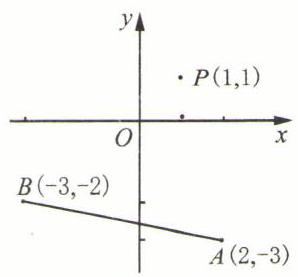
\includegraphics[width=0.2\textwidth]{bodyxb/src/bo_d20cdrf7aajc73bfmvhg_25_1124_754_298_277_0.jpg}
\end{center}


(第 14 题)

$\left\lbrack  {\arctan \dfrac{3}{4},\arctan \left( {-4}\right)  + \pi }\right\rbrack$ ,对应斜率 $k \geq  \dfrac{3}{4}$ 或 $k \leq   - 4$ .

15. A 提示: 将横坐标 ${x}_{1},{x}_{2}$ 分别代入 $y = {kx} + b$ ,得 $P\left( {{x}_{1},k{x}_{1} + b}\right) ,Q\left( {{x}_{2},k{x}_{2} + b}\right)$ ,

$\therefore \;\left| {PQ}\right|  = \sqrt{{\left( {x}_{2} - {x}_{1}\right) }^{2} + {k}^{2}{\left( {x}_{2} - {x}_{1}\right) }^{2}} = \sqrt{1 + {k}^{2}}\left| {{x}_{1} - {x}_{2}}\right|$ .

16. (1) $\left\lbrack  {0,\dfrac{\pi }{4}}\right\rbrack   \cup  \left\lbrack  {\dfrac{3}{4}\pi ,\pi }\right)$ 提示: ${k}_{OA} = \dfrac{1 - 0}{1 - 0} = 1,{k}_{OB} = \dfrac{-1 - 0}{1 - 0} =  - 1$ ,如图 (1),直线 $l$ 的倾斜角的取值范围是 $\left\lbrack  {0,\arctan 1}\right\rbrack   \cup  \lbrack \arctan \left( {-1}\right)  + \pi ,\pi )$ ,即 $\left\lbrack  {0,\dfrac{\pi }{4}}\right\rbrack   \cup  \left\lbrack  {\dfrac{3}{4}\pi ,\pi }\right)$ .

(2) $\left( {0,\dfrac{\pi }{6}\rbrack \cup \lbrack \dfrac{5}{6}\pi ,\pi }\right)$ 提示: $- \sqrt{3}\sin \theta  = 0 \Leftrightarrow  \sin \theta  = 0 \Leftrightarrow  {\cos }^{2}\theta  = 1$ .

\begin{center}
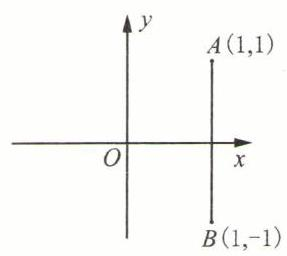
\includegraphics[width=0.2\textwidth]{bodyxb/src/bo_d20cdrf7aajc73bfmvhg_25_1135_1125_287_256_0.jpg}
\end{center}


[第 16(1)题]

$\because A,B$ 是相异的两点, $\therefore  - \sqrt{3}\sin \theta  \neq  0$ ,即 $A,B$ 两点的横坐标不同, ${k}_{AB}$ 存在.

${k}_{AB} = \dfrac{1 - {\cos }^{2}\theta }{0 - \left( {-\sqrt{3}\sin \theta }\right) } = \dfrac{{\sin }^{2}\theta }{\sqrt{3}\sin \theta } = \dfrac{\sin \theta }{\sqrt{3}}$ ,其中 $\sin \theta  \in  \left\lbrack  {-1,0)\cup (0,1}\right\rbrack$ .

$\therefore {k}_{AB} \in  \left\lbrack  {-\dfrac{1}{\sqrt{3}},0}\right)  \cup  \left( {0,\dfrac{1}{\sqrt{3}}}\right\rbrack  ,\;\therefore$ 直线 ${AB}$ 的倾斜角的取值范围为 $\left( {0,\arctan \dfrac{1}{\sqrt{3}}}\right\rbrack   \cup  \left\lbrack  {\arctan \left( {-\dfrac{1}{\sqrt{3}}}\right)  + \pi ,\pi }\right) ,$ 即 $\left( {0,\dfrac{\pi }{6}}\right\rbrack   \cup  \left\lbrack  {\dfrac{5}{6}\pi ,\pi }\right) .$

(3) $\left\lbrack  {0,\dfrac{\pi }{3}}\right\rbrack   \cup  \left( {\dfrac{\pi }{2},\pi }\right)$ 提示: $\alpha  \in  \lbrack 0,\pi )$ ,结合 $\tan \alpha  \leq  \sqrt{3},\therefore \alpha  \in  \left\lbrack  {0,\arctan \sqrt{3}}\right\rbrack   \cup  \left( {\dfrac{\pi }{2},\pi }\right)$ ,

$\therefore \alpha  \in  \left\lbrack  {0,\dfrac{\pi }{3}}\right\rbrack   \cup  \left( {\dfrac{\pi }{2},\pi }\right)$ .

17. (1) $\theta  = \dfrac{k\pi }{2},k \in  \mathbf{Z}$ 提示: $\because {\sin }^{2}\theta  \in  \left\lbrack  {0,1}\right\rbrack  ,\therefore A,B,C$ 三点的横坐标各不相同, $A,B,C$ 所在直线的斜率存在. ${k}_{AL}$  $= \dfrac{-\dfrac{2}{3} - {\cos }^{2}\theta }{{\sin }^{2}\theta  - 2} = \dfrac{\dfrac{2}{3} + {\cos }^{2}\theta }{2 - 1 + {\cos }^{2}\theta } = \dfrac{{\cos }^{2}\theta  + \dfrac{2}{3}}{{\cos }^{2}\theta  + 1},{k}_{AC} = \dfrac{-4 - {\cos }^{2}\theta }{-4 - 2} = \dfrac{{\cos }^{2}\theta  + 4}{6},{k}_{AB} = {k}_{AC}$ . 有 $\dfrac{{\cos }^{2}\theta  + \dfrac{2}{3}}{{\cos }^{2} + 1} = \dfrac{{\cos }^{2}\theta  + 4}{6}$ ,令 $t =$

${\cos }^{2}\theta$ ,整理得 ${t}^{2} - t = 0,{t}_{1} = 0,{t}_{2} = 1$ . 当 ${t}_{1} = 0$ 时, ${\cos }^{2}\theta  = 0,\cos \theta  = 0,\theta  = \dfrac{\pi }{2} + {k}_{1}\pi \left( {{k}_{1} \in  }\right.$  $\mathbf{Z})$ ；当 ${t}_{2} = 1$ 时, ${\cos }^{2}\theta  = 1,{\sin }^{2}\theta  = 0,\theta  = {k}_{2}\pi \left( {{k}_{2} \in  \mathbf{Z}}\right) ,\;\therefore \;\theta  = \dfrac{k}{2}\pi \left( {k \in  \mathbf{Z}}\right)$ .

\begin{center}
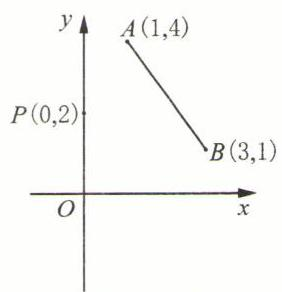
\includegraphics[width=0.2\textwidth]{bodyxb/src/bo_d20cdrf7aajc73bfmvhg_25_1139_1806_282_292_0.jpg}
\end{center}


[第 17(2)题]

(2) $- \dfrac{1}{3} \leq  a \leq  2$ 提示:直线 $y = {ax} + 2$ 是过点 $P\left( {0,2}\right)$ ,斜率为 $a$ 的直线. ${k}_{PA} = \dfrac{4 - 2}{1 - 0} = 2$ , ${k}_{PB} = \dfrac{1 - 2}{3 - 0} =  - \dfrac{1}{3}$ . 如图,直线 $y = {ax} + 2$ 的倾斜角范围为: $\left\lbrack  {0,\arctan 2}\right\rbrack   \cdot  \mathrm{U}$  $\left\lbrack  {\arctan \left( {-\dfrac{1}{3}}\right)  + \pi ,\pi }\right)$ ,对应地,斜率 $a$ 的取值范围是 $a \in  \left\lbrack  {-\dfrac{1}{3},2}\right\rbrack$ .

(3) $- \dfrac{2}{3}$ 提示: 把直线写为斜截式,即 $y =  - \dfrac{2{a}^{2} - {7a} + 3}{{a}^{2} - 9}x - \dfrac{3{a}^{2}}{{a}^{2} - 9}$ ,

由题意 $\left\{  {\begin{array}{l} \dfrac{-2{a}^{2} + {7a} - 3}{{a}^{2} - 9} = \tan \dfrac{\pi }{4} = 1, \\  {a}^{2} - 9 \neq  0. \end{array}\therefore a =  - \dfrac{2}{3}\left( {a = 3}\right. }\right.$ 不满足 $\left. {{a}^{2} - 9 \neq  0\text{ ,舍去 }}\right)$ .

18. 由 $\dfrac{2\sin \alpha  - \cos \alpha }{5\cos \alpha  + 3\sin \alpha } = \dfrac{3}{11}$ ,可得 $\sin \alpha  = 2\cos \alpha ,\therefore \tan \alpha  = 2.\therefore$ 直线 $l$ 的方程为 $y = 2\left( {x + 2}\right)  = {2x} + 4$ ,即 $l : {2x} - y + 4$  $= 0$ .

19. (1) 外心 $M$ 是 $\bigtriangleup {ABC}$ 三边的垂直平分线的交点,易知线段 ${AB}$ 的垂直平分线是 $x = 4$ . 下面求线段 ${AC}$ 的垂直平分线,线段 ${AC}$ 中点为 $\left( {\dfrac{7}{2},3}\right) ,{k}_{AC} = \dfrac{6}{7}$ ,故垂直平分线的斜率是 $- \dfrac{7}{6}.\therefore$ 线段 ${AC}$ 的垂直平分线的方程为 $y - 3 =$  $- \dfrac{7}{6}\left( {x - \dfrac{7}{2}}\right)$ ,即 ${14x} + {12y} - {85} = 0$ . 联立 $\left\{  \begin{array}{l} x = 4, \\  {14x} + {12y} - {85} = 0, \end{array}\right.$ 解得 $\left\{  {\begin{array}{l} x = 4, \\  y = \dfrac{29}{12}. \end{array}\;\therefore \;\text{ 外心 }M}\right.$ 的坐标为 $M\left( {4,\dfrac{29}{12}}\right)$ .

对于垂心 $H$ ,可得边 ${AB}$ 上的高所在的直线方程为 $x = 7$ . 下面求边 ${AC}$ 上的高所在直线,这条直线经过点 $B$ ,斜率为 $- \dfrac{7}{6}$ ,故有方程: $y - 0 =  - \dfrac{7}{6}\left( {x - 8}\right)$ ,代入 ${x}_{H} = 7$ ,有 ${y}_{H} = \dfrac{7}{6},\therefore$ 垂心 $H$ 的坐标为 $H\left( {7,\dfrac{7}{6}}\right)$ . 重心 $G$ 的坐标为 $G\left( {\dfrac{0 + 8 + 7}{3},\dfrac{0 + 0 + 6}{3}}\right)$ ,即 $G\left( {5,2}\right)$ .

(2)先求 ${HG}$ 所在直线方程, ${k}_{HG} = \dfrac{2 - \dfrac{7}{6}}{5 - 7} =  - \dfrac{5}{12},\therefore {l}_{HG} : y - 2 =  - \dfrac{5}{12}\left( {x - 5}\right)$ ,代入 ${x}_{M} = 4$ ,求得 $y = 2 + \dfrac{5}{12} = \dfrac{29}{12} =$  ${y}_{M}$ . 点 $M$ 在直线 ${HG}$ 上, $\therefore M,H,G$ 三点共线,证毕.

20. 设点 $P$ 的坐标为 $P\left( {x,y}\right) ,{\left| AP\right| }^{2} + {\left| BP\right| }^{2} + {\left| CP\right| }^{2} = \mathop{\sum }\limits_{{i = 1}}^{3}\left\lbrack  {{\left( x - {x}_{i}\right) }^{2} + {\left( y - {y}_{i}\right) }^{2}}\right\rbrack   = \mathop{\sum }\limits_{{i = 1}}^{3}\left\lbrack  {{x}^{2} - 2{x}_{i}x + {x}_{i}{}^{2} + {y}^{2} - 2{y}_{i}y + }\right.$  $\left. {{y}_{i}{}^{2}}\right\rbrack   = 3{x}^{2} - {2x} \cdot  \mathop{\sum }\limits_{{i = 1}}^{3}{x}_{i} + \mathop{\sum }\limits_{{i = 1}}^{3}{x}_{i}{}^{2} + 3{y}^{2} - {2y}\mathop{\sum }\limits_{{i = 1}}^{3}{y}_{i} + \mathop{\sum }\limits_{{i = 1}}^{3}{y}_{i}{}^{2}$ ,其中 $3{x}^{2} - {2x}\mathop{\sum }\limits_{{i = 1}}^{3}{x}_{i} = 3\left\lbrack  {{x}^{2} - \left( {\dfrac{2}{3}\mathop{\sum }\limits_{{i = 1}}^{3}{x}_{i}}\right) x + {\left( \dfrac{1}{3}\mathop{\sum }\limits_{{i = 1}}^{3}{x}_{i}\right) }^{2}}\right\rbrack   -$  $\dfrac{1}{3}{\left( \mathop{\sum }\limits_{{i = 1}}^{3}{x}_{i}\right) }^{2} = 3{\left\lbrack  x - \dfrac{1}{3}\mathop{\sum }\limits_{{i = 1}}^{3}{x}_{i}\right\rbrack  }^{2} - \dfrac{1}{3}{\left( \mathop{\sum }\limits_{{i = 1}}^{3}{x}_{i}\right) }^{2} \geq   - \dfrac{1}{3}{\left( \mathop{\sum }\limits_{{i = 1}}^{3}{x}_{i}\right) }^{2}$ . 此时 $x = \dfrac{1}{3}\mathop{\sum }\limits_{{i = 1}}^{3}{x}_{i}$ . 同样地, $3{y}^{2} - {2y}\mathop{\sum }\limits_{{i = 1}}^{3}{y}_{i} = 3{\left\lbrack  y - \dfrac{1}{3}\mathop{\sum }\limits_{{i = 1}}^{3}{y}_{i}\right\rbrack  }^{2}$  $- \dfrac{1}{3}{\left( \mathop{\sum }\limits_{{i = 1}}^{3}{y}_{i}\right) }^{2} \geq   - \dfrac{1}{3}{\left( \mathop{\sum }\limits_{{i = 1}}^{3}{y}_{i}\right) }^{2}$ . 此时 $y = \dfrac{1}{3}\mathop{\sum }\limits_{{i = 1}}^{3}{y}_{i}$ .

$\therefore$ 当取 $P\left( {\dfrac{{x}_{1} + {x}_{2} + {y}_{3}}{3},\dfrac{{y}_{1} + {y}_{2} + {y}_{3}}{3}}\right)$ 时, ${\left| AP\right| }^{2} + {\left| BP\right| }^{2} + {\left| CP\right| }^{2}$ 的值最小,为 $\mathop{\sum }\limits_{{i = 1}}^{3}{x}_{i}{}^{2} - \dfrac{1}{3}{\left( \mathop{\sum }\limits_{{i = 1}}^{3}{x}_{i}\right) }^{2} + \mathop{\sum }\limits_{{i = 1}}^{3}{y}_{i}{}^{2}$  $- \dfrac{1}{3}{\left( \mathop{\sum }\limits_{{i = 1}}^{3}{y}_{i}\right) }^{2}$ .

21. A 提示: 利用直线方程的截距式,有 $\dfrac{x}{-2} + \dfrac{y}{3} = 1$ ,即 ${3x} - {2y} + 6 = 0$ .

22. $C$ 提示:将(3,0)代入直线方程,有 $3\left( {m + 2}\right)  = {2m},\;\therefore m =  - 6$ .

23. D 提示: ${3x} - {2y} = 4,\therefore \dfrac{3}{4}x - \dfrac{1}{2}y = 1$ ,截距式方程为 $\dfrac{x}{\dfrac{4}{3}} + \dfrac{y}{-2} = 1$ .

24. D 提示: 设该截距为 $t$ . 情况一: $t = 0$ ,即直线过原点(0,0),直线方程为 $\dfrac{y - 0}{-4 - 0} = \dfrac{x - 0}{3 - 0}$ ,即 ${4x} + {3y} = 0$ .

情况二: $t \neq  0$ ,直线方程可写为 $\dfrac{x}{t} + \dfrac{y}{t} = 1$ ,代入(3, - 4),得 $\dfrac{3}{t} - \dfrac{4}{t} = 1,\;\therefore \;t =  - 1$ . 此时直线方程为 $x + y + 1 = 0$ . 综合两种情况, 选 D.

25. (1) ${2x} + y - 8 = 0$ 提示: 设直线与坐标轴交于 $\left( {a,0}\right) ,\left( {0,b}\right)$ ,则 $\left\{  \begin{array}{l} \dfrac{a + 0}{2} = 2, \\  \dfrac{0 + b}{2} = 4, \end{array}\right.$ 解得 $\left\{  \begin{array}{l} a = 4, \\  b = 8. \end{array}\right.$

直线的方程为 $\dfrac{x}{4} + \dfrac{y}{8} = 1$ ,即 ${2x} + y - 8 = 0$ .

(2) ${3x} - {2y} + {12} = 0$ 或 $x + y - 1 = 0$ 提示:设直线方程为 $\dfrac{x}{a} + \dfrac{y}{b} = 1$ (直线不可能过原点). 由题意 $\left\{  \begin{array}{l} a + b = 2, \\   - \dfrac{2}{a} + \dfrac{3}{b} = 1, \end{array}\right.$ 解得 $\left\{  \begin{array}{l} a =  - 4, \\  b = 6. \end{array}\right.$ 或 $\left\{  {\begin{array}{l} a = 1, \\  b = 1. \end{array}\therefore }\right.$ 直线方程为 $\dfrac{x}{-4} + \dfrac{y}{6} = 1$ 或 $\dfrac{x}{1} + \dfrac{y}{1} = 1$ ,即 ${3x} - {2y} + {12} = 0$ 或 $x + y - 1 = 0$ .

(3) $a =  - 2$ 提示: 将 $\dfrac{a}{3}x - {2y} - {4a} = 0$ 转化为 $\dfrac{x}{12} + \dfrac{y}{-{2a}} = 1$ ,由题意得 ${12} = 3 \cdot  \left( {-{2a}}\right) ,\therefore a =  - 2$ .

26. 设直线的方程为 $y = \dfrac{1}{6}x + b$ ,当 $x = 0$ 时 $y = b$ ; 当 $y = 0$ 时 $x =  - {6b}$ ,即过点(0, b)和(-6b,0).

由题意 $\dfrac{1}{2}\left| b\right|  \cdot  \left| {-{6b}}\right|  = 3{b}^{2} = 3,\;\therefore \;b =  \pm  1$ ,

$\therefore$ 直线的方程为 $y = \dfrac{1}{6}x + 1$ 或 $y = \dfrac{1}{6}x - 1$ ,即 $x - {6y} + 6 = 0$ 或 $x - {6y} - 6 = 0$ .

27. (1) 设顶点 $C$ 的坐标为 $C\left( {x,y}\right) ,\therefore {AC}$ 的中点 $M$ 的坐标为 $M\left( {\dfrac{5 + x}{2},\dfrac{y - 2}{2}}\right) ,{BC}$ 的中点 $N$ 的坐标为 $N\left( {\dfrac{7 + x}{2},\dfrac{3 + y}{2}}\right)$ . 由题意 $\left\{  \begin{array}{l} \dfrac{5 + x}{2} = 0, \\  \dfrac{3 + y}{2} = 0, \end{array}\right.$ 解得 $\left\{  \begin{array}{l} x =  - 5, \\  y =  - 3. \end{array}\right. \;\therefore \;$ 顶点 $C$ 的坐标为 $C\left( {-5, - 3}\right)$ .

(2)此时有 $M\left( {0, - \dfrac{5}{2}}\right) ,N\left( {1,0}\right)$ . 利用直线的截距式,直线 ${MN}$ 的方程为 $\dfrac{x}{1} + \dfrac{y}{-\dfrac{5}{2}} = 1$ ,即 ${5x} - {2y} - 5 = 0$ .

28. C 提示: 如图,作 $N$ 关于 $x$ 轴的对称点 ${N}^{\prime }\left( {5,2}\right) ,\left| \right| {PM}\left| -\right| {PN}\left| \right|  =$  $\left| \right| {PM}\left| -\right| P{N}^{\prime }\left| \right|  \leq  \left| {M{N}^{\prime }}\right|$ ,当且仅当 $P$ 为直线 $M{N}^{\prime }$ 与 $x$ 轴交点时,等号成立. ${l}_{M{N}^{\prime }}$ : $\dfrac{y - 3}{2 - 3} = \dfrac{x - 1}{5 - 1}$ ,即 $x + {4y} - {13} = 0$ . 代入 $y = 0$ ,得 $x = {13}$ . 即点 $P$ 的坐标是(13,0)时, ${\left| \left| PM\right|  - \left| PN\right| \right| }_{\max } = \left| {M{N}^{\prime }}\right| .$

\begin{center}
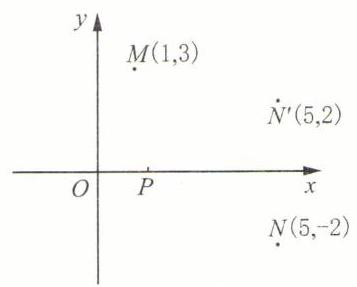
\includegraphics[width=0.3\textwidth]{bodyxb/src/bo_d20cdrf7aajc73bfmvhg_27_1059_723_357_287_0.jpg}
\end{center}


(第 28 题)

29. D 提示: 对于 $A$ : 在 $\dfrac{y - {y}_{1}}{x - {x}_{1}} = k$ 中,当 $x - {x}_{1} \neq  0$ ,即 $x \neq  {x}_{1}$ 时,才有 $y - {y}_{1} = k\left( {x - {x}_{1}}\right)$ ,因此 $\dfrac{y - {y}_{1}}{x - {x}_{1}} = k$ 表示的是过点 $\left( {{x}_{1},{y}_{1}}\right)$ 且斜率为 $k$ 的直线并去掉 $\left( {{x}_{1},{y}_{1}}\right)$ 点的图形,错误.

对于 $B : b$ 是直线 $y = {kx} + b$ 在 $y$ 轴上的截距,可正可负. $b < 0$ 时, $b = \left| {OB}\right|$ 应为 $\left| b\right|  = {OB}$ ,错误.

对于 $C$ : 若 $a = b = 0$ ,则直线方程不能写为 $\dfrac{x}{a} + \dfrac{y}{b} = 1$ 的形式,错误.

对于 $D$ : 由于 ${P}_{1},{P}_{2}$ 是两个不同的点,故 ${x}_{1} \neq  {x}_{2},{y}_{1} \neq  {y}_{2}$ 至少有一个成立. 当 ${x}_{1} \neq  {x}_{2}$ 时,有 $y - {y}_{1} = \dfrac{{y}_{2} - {y}_{1}}{{x}_{2} - {x}_{1}}\left( {x - {x}_{1}}\right)$ ,

表示过 ${P}_{1}\left( {{x}_{1},{y}_{1}}\right) ,{P}_{2}\left( {{x}_{2},{y}_{2}}\right)$ 的一条直线. 当 ${y}_{1} \neq  {y}_{2}$ 时,若 ${x}_{1} = {x}_{2}$ ,则直线方程为 $x = {x}_{1},\left( {{x}_{2} - {x}_{1}}\right) \left( {y - {y}_{1}}\right)  = \left( {{y}_{2} - }\right.$  $\left. {y}_{1}\right) \left( {x - {x}_{1}}\right)$ 也可化为 $x = {x}_{1}$ ,而若 ${x}_{1} \neq  {x}_{2}$ 时,有 $\dfrac{y - {y}_{1}}{{y}_{2} - {y}_{1}} = \dfrac{x - {x}_{1}}{{x}_{2} - {x}_{1}}$ ,此即过点 ${P}_{1}\left( {{x}_{1},{y}_{1}}\right) ,{P}_{2}\left( {{x}_{2},{y}_{2}}\right)$ 的直线的两点式, 正确. 故选 D. 30. $C$ 提示: ${l}_{1},{l}_{2},{l}_{3}$ 的斜截式为: ${l}_{1} : y = \dfrac{1}{2}x + {2a},{l}_{2} : y = x - {6a},{l}_{3} : y = {2x} - {4a}$ .

对于(A): 设 ${l}_{1},{l}_{2},{l}_{3}$ 的倾斜角分别为 ${\alpha }_{1},{\alpha }_{2},{\alpha }_{3}$ ,则 $\tan {\alpha }_{1} = \dfrac{1}{2},\tan {\alpha }_{2} = 1,\tan {\alpha }_{3} = 2,{\alpha }_{1} + {\alpha }_{3} = \dfrac{\pi }{2},{\alpha }_{2} = \dfrac{\pi }{4}$ ,

$\therefore {\alpha }_{1} + {\alpha }_{2} + {\alpha }_{3} = \dfrac{3}{4}\pi  \neq  \dfrac{\pi }{2}$ ,错误.

对于(B): ${b}_{1} = {2a},{b}_{2} =  - {6a},{b}_{3} =  - {4a},{b}_{1} + {b}_{3} =  - {2a},2{b}_{2} =  - {12a},\;\therefore {b}_{1} + {b}_{3} \neq  2{b}_{2}\left( {a \neq  0}\right)$ ,错误.

对于(C): 根据对(A)中的讨论有: ${\alpha }_{1} + {\alpha }_{3} = \dfrac{\pi }{2} = 2{\alpha }_{2} = \dfrac{\pi }{2}$ ,正确.

对于(D):截距之和为 $- {4a} + {6a} + {2a} = {4a} \neq  {12}\left| a\right| \left( {a \neq  0}\right)$ ,错误.

31. (1) $\because \cos \alpha  =  - \dfrac{4}{5}$ 且 $\alpha  \in  \lbrack 0,\pi ),\therefore \sin \alpha  = \dfrac{3}{5},\tan \alpha  =  - \dfrac{3}{4}$ . 设直线 $l$ 的方程为

$y =  - \dfrac{3}{4}x + b$ ,当 $x = 0$ 时, $y = b$ ; 当 $y = 0$ 时, $x = \dfrac{4}{3}b$ . 由题意, $b + \dfrac{4}{3}b = 1,\;\therefore \;b = \dfrac{3}{7},\;\therefore$ 直线 $l$ 的方程为

$y =  - \dfrac{3}{4}x + \dfrac{3}{7}$ ,即 $l : {21x} + {28y} - {12} = 0.$

(2)由题意, $l$ 在 $x$ 轴、 $y$ 轴上的截距存在,分别设为 $a,b$ ,则有 $\left\{  \begin{array}{l} \left| a\right|  = \left| b\right| , \\  \dfrac{1}{2}\left| a\right|  \cdot  \left| b\right|  = {18}. \end{array}\right.$

$\therefore \left| a\right|  = \left| b\right|  = 6$ . 直线 $l$ 的方程为 $\dfrac{x}{a} + \dfrac{y}{b} = 1$ ,其中 $a =  \pm  6,b =  \pm  6$ .

共有 4 种情况: $x + y - 6 = 0,x - y - 6 = 0,x - y + 6 = 0,x + y + 6 = 0$ .

(3)设 $A\left( {a,0}\right) ,B\left( {0,b}\right) ,{ab} \neq  0\because \left| {AP}\right|  : \left| {PB}\right|  = 5 : 3\therefore \left| \vv{AP}\right|  = \dfrac{5}{3}\left| \vv{PB}\right|$ .

情况一: $\vv{AP} = \dfrac{5}{3}\vv{PB}$ ,则考虑点 $P$ 的坐标,有 $\left\{  \begin{array}{l} \dfrac{6}{1 + \dfrac{5}{3}} =  - 4, \\  \dfrac{5}{3}b = 3, \\  \dfrac{5}{1 + \dfrac{5}{3}} = 3, \end{array}\right.$ 解得 $\left\{  \begin{array}{l} a =  - \dfrac{32}{3}, \\  b = \dfrac{24}{5}. \end{array}\right.$ 此时, $l : \dfrac{x}{-\dfrac{32}{3}} + \dfrac{y}{\dfrac{24}{5}} = 1$ ,即 ${9x} - {20y} + {96} = 0$

情况二: $\vv{AP} =  - \dfrac{5}{3}\vv{PB}$ ,则考虑点 $P$ 的坐标,有 $\left\{  \begin{array}{l} \dfrac{a}{1 - \dfrac{5}{3}} =  - 4, \\  \dfrac{-\dfrac{5}{3}}{1 - \dfrac{5}{3}} = 3, \\  1 - \dfrac{5}{3} = 3, \end{array}\right.$ 解得 $\left\{  \begin{array}{l} a = \dfrac{8}{3}, \\  b = \dfrac{6}{5}. \end{array}\right.$ 此时, $l : \dfrac{x}{3} + \dfrac{y}{6} = 1$ ,

即 ${9x} + {20y} - {24} = 0,\therefore$ 直线 $l$ 的方程为 ${9x} - {20y} + {96} = 0$ 或 ${9x} + {20y} - {24} = 0$ .

(4)如图,设 $l$ 交 ${AC}$ 于点 $P$ , $l$ 交 ${CB}$ 于点 $Q$ .

\begin{center}
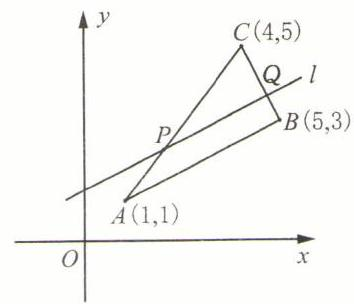
\includegraphics[width=0.3\textwidth]{bodyxb/src/bo_d20cdrf7aajc73bfmvhg_28_1155_750_354_304_0.jpg}
\end{center}


[第 31(4)题]

由题意, $\dfrac{{S}_{\bigtriangleup {CPQ}}}{{S}_{\bigtriangleup {CAB}}} = \dfrac{1}{2},\bigtriangleup {CPQ} \backsim  \bigtriangleup {CAB}$ .

$\therefore \dfrac{{S}_{\bigtriangleup {CPQ}}}{{S}_{\bigtriangleup {CAB}}} = {\left( \dfrac{\left| CP\right| }{\left| CA\right| }\right) }^{2} = \dfrac{1}{2},\dfrac{\left| CP\right| }{\left| CA\right| } = \dfrac{\sqrt{2}}{2}$ ,

$\therefore \vv{AP} = \dfrac{2 - \sqrt{2}}{\sqrt{2}}\vv{PC} = \left( {\sqrt{2} - 1}\right) \vv{PC}$

$\therefore$ 点 $P$ 的坐标为 $\left( {\dfrac{1 + \left( {\sqrt{2} - 1}\right)  \cdot  4}{1 + \left( {\sqrt{2} - 1}\right) },\dfrac{1 + \left( {\sqrt{2} - 1}\right)  \cdot  5}{1 + \left( {\sqrt{2} - 1}\right) }}\right)$ ,

即 $P\left( {4 - \dfrac{3}{2}\sqrt{2},5 - 2\sqrt{2}}\right) .\because l//{AB},\therefore \;{k}_{l} = {k}_{AB} = \dfrac{3 - 1}{5 - 1} = \dfrac{1}{2}$ .

$\therefore l : y - \left( {5 - 2\sqrt{2}}\right)  = \dfrac{1}{2}\left\lbrack  {x - \left( {4 - \dfrac{3}{2}\sqrt{2}}\right) }\right\rbrack$ ,即 ${2x} - {4y} + {12} - 5\sqrt{2} = 0.$

32. 由题意,设点 $Q$ 的坐标为 $Q\left( {t,{4t}}\right) \left( {t > 0}\right)$ . 设点 $M$ 的坐标为 $M\left( {m,0}\right) \vv{PQ} = \left( {t,{4t}}\right)  - \left( {6,4}\right)  = \left( {t - 6,{4t} - 4}\right) ,\vv{MP} = \left( {6,4}\right)$  $- \left( {m,0}\right)  = \left( {6 - m,4}\right) .\because M,P,Q$ 三点共线,故存在唯一实数 $\lambda$ ,使得 $\vv{PQ} = \lambda \vv{MP}$ ,则 $\left\{  \begin{array}{l} t - 6 = \lambda \left( {6 - m}\right) , \\  {4t} - 4 = {4\lambda }. \end{array}\right.$ 消去 $\lambda$ ,有 $t -$  $6 = \left( {t - 1}\right) \left( {6 - m}\right)$ . 当 $t = 1$ 时,点 $Q$ 的坐标为 $\left( {1,4}\right) ,{PQ}//x$ 轴,与 $x$ 轴无交点,故 $t \neq  1.\therefore m = \dfrac{5t}{t - 1} > 0$ ,得 $t > 1$ . ${S}_{\bigtriangleup {OMQ}} = \dfrac{1}{2}m \cdot  {4t} = \dfrac{{10}{t}^{2}}{t - 1} = \dfrac{{10}{\left\lbrack  \left( t - 1\right)  + 1\right\rbrack  }^{2}}{t - 1} = {10} \cdot  \left\lbrack  {\left( {t - 1}\right)  + \dfrac{1}{t - 1} + 2}\right\rbrack   \geq  {10} \cdot  \left\lbrack  {2\sqrt{\left( {t - 1}\right)  \cdot  \dfrac{1}{t - 1}} + 2}\right\rbrack   = {40}$ . 当且仅当 $t$  $- 1 = \dfrac{1}{t - 1}$ ,即 $t = 2$ 时等号成立. 此时点 $Q$ 的坐标为 $Q\left( {2,8}\right)$ .

33. D 提示: 将直线方程写为 $y =  - \dfrac{1}{\sqrt{3}}x - \dfrac{1}{\sqrt{3}}$ ,倾斜角为 $\arctan \left( {-\dfrac{1}{\sqrt{3}}}\right)  + \pi  = \pi  - \arctan \dfrac{\sqrt{3}}{3} = \pi  - \dfrac{\pi }{6} = \dfrac{5}{6}\pi$ .

34. $D$ 提示: 在 ${ax} + {by} + c = 0$ 中,令 $x = 0$ ,则 $y =  - \dfrac{c}{b} < 0$ . 令 $y = 0$ ,则 $x =  - \dfrac{c}{a} < 0$ . 即 ${ax} + {by} + c = 0$ 在 $x$ 轴, $y$ 轴上的截距均小于 0 .

\begin{center}
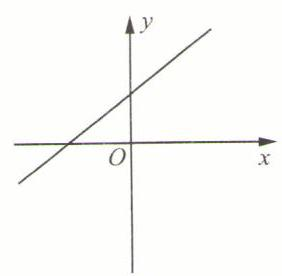
\includegraphics[width=0.2\textwidth]{bodyxb/src/bo_d20cdrf7aajc73bfmvhg_28_1236_1776_282_276_0.jpg}
\end{center}


(第 35 题)

35. A 提示: 在 ${ax} + {by} + c = 0$ 中,令 $x = 0$ ,则 $y =  - \dfrac{c}{b} > 0$ . 令 $y = 0$ ,则 $x =  - \dfrac{c}{a}$ .

$\because {ab} < 0,{bc} < 0,\;\therefore \;a{b}^{2}c > 0 \Rightarrow  {ac} > 0,\;\therefore \;x =  - \dfrac{c}{a} < 0$ ,直线经过 $\left( {0, - \dfrac{c}{b}}\right)$ 和 $\left( {-\dfrac{c}{a},0}\right)$ ,如图,直线经第一、二、三象限.

36. $B$ 提示: $b \neq  0$ ,故将 ${ax} - {by} - c = 0$ 写为 $y = \dfrac{a}{b}x - \dfrac{c}{b}$ , $\because {ab} < 0$ ,

$\therefore \dfrac{a}{b} < 0$ . 倾斜角为 $\arctan \dfrac{a}{b} + \pi$ ,范围为 $\left( {\dfrac{\pi }{2},\pi }\right)$ .

37. A 提示: 由题意,对直线 ${ax} - y + 2 = 0$ 上任意一点 $\left( {p,{ap} + 2}\right)$ ,关于直线 $y = x$ 的对称点 $\left( {{ap} + 2,p}\right)$ 在直线 ${3x} - y - b$  $= 0$ 上, $\therefore 3\left( {{ap} + 2}\right)  - p - b = 0$ ,即 $\left( {{3a} - 1}\right) p + 6 - b = 0$ 对任意 $p$ 恒成立, $\therefore \left\{  \begin{array}{l} {3a} - 1 = 0, \\  6 - b = 0, \end{array}\right.$ 解得 $\left\{  \begin{array}{l} a = \dfrac{1}{3}, \\  b = 6. \end{array}\right.$

38. B 提示: 作变量替换: $\left\{  \begin{array}{l} {x}^{\prime } = x - 1, \\  {y}^{\prime } = y - 1, \end{array}\right.$ 即 $\left\{  \begin{array}{l} x = {x}^{\prime } + 1, \\  y = {y}^{\prime } + 1. \end{array}\right.$ 相当于作了平移变换,此时有 $\left| {x}^{\prime }\right|  + \left| {y}^{\prime }\right|  =$ 1,定义函数 $u\left( t\right)  = \left\{  \begin{array}{l} 1\;t \geq  0, \\   - 1\;t < 0. \end{array}\right.$ 则可把 $\left| {x}^{\prime }\right|  + \left| {y}^{\prime }\right|  = 1$ 写为 $\dfrac{{x}^{\prime }}{u\left( {x}^{\prime }\right) } + \dfrac{{y}^{\prime }}{u\left( {y}^{\prime }\right) } = 1$ 的截距式形式. 由图,当 ${x}^{\prime } \geq  0,{y}^{\prime } \geq  0$ 时,有 $\dfrac{{x}^{\prime }}{1} + \dfrac{{y}^{\prime }}{1} = 1$ ,对应线段 ${AB}$ ；当 ${x}^{\prime } \geq  0,{y}^{\prime } < 0$ 时,有 $\dfrac{{x}^{\prime }}{1} + \dfrac{{y}^{\prime }}{-1} = 1$ ,对应线段 ${AD}$ (不含点 $A$ )；当 ${x}^{\prime } < 0,{y}^{\prime } \geq  0$ 时,有 $\dfrac{{x}^{\prime }}{-1} + \dfrac{{y}^{\prime }}{1} = 1$ ,对应线段 ${BC}$ (不含点 $B$ )；当 ${x}^{\prime } <$  $0,{y}^{\prime } < 0$ 时,有 $\dfrac{{x}^{\prime }}{-1} + \dfrac{{y}^{\prime }}{-1} = 1$ ,对应线段 ${CD}$ (不含点 $C,D$ ). 由于图形平移不改变图形的面积, 故原方程确定的曲线所围成的图形面积为 $4 \times  \dfrac{1}{2} \times  1 \times  1 = 2$ .

\begin{center}
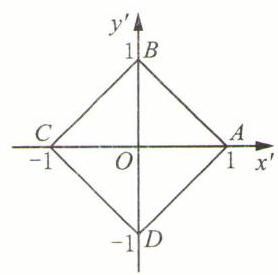
\includegraphics[width=0.2\textwidth]{bodyxb/src/bo_d20cdrf7aajc73bfmvhg_29_1134_290_278_275_0.jpg}
\end{center}


(第 38 题)

39. B 提示:集合 $U$ 表示平面直角坐标系 ${xOy}$ 上所有的点,集合 $M$ 中: $\dfrac{y - 3}{x - 2} = 1 \Leftrightarrow  y - 3 = x - 2$ 且 $x \neq  2 \Leftrightarrow  y = x + 1$ 且 $x \neq$ 2. $M$ 可以写成 $M = \{ \left( {x,y}\right)  \mid  y = x + 1$ 且 $\left( {x,y}\right)  \neq  \left( {2,3}\right) \} ,N = \{ \left( {x,y}\right)  \mid  y \neq  x + 1\} .M \cup  N$ 表示平面直角坐标系中除点 (2,3)外的所有点. $\therefore \overline{M \cup  N} = \{ \left( {2,3}\right) \}$ .

40. (1) $x - y - \sqrt{3} = 0$ 提示: 设直线 $x - y + \sqrt{3} = 0$ 上任意一点(x, y)关于原点中心对称的点为 $\left( {{x}^{\prime },{y}^{\prime }}\right)$ ,则 $\left\{  \begin{array}{l} {x}^{\prime } =  - x, \\  {y}^{\prime } =  - y, \end{array}\right.$

$\therefore \left\{  \begin{array}{l} x =  - {x}^{\prime }, \\  y =  - {y}^{\prime }. \end{array}\right.$ 代入 $x - y + \sqrt{3} = 0$ ,得 $- {x}^{\prime } + {y}^{\prime } + \sqrt{3} = 0$ ,即 ${x}^{\prime } - {y}^{\prime } - \sqrt{3} = 0$ .

$\therefore$ 原直线关于原点成中心对称的直线方程是 $x - y - \sqrt{3} = 0$ .

(2) $y = \dfrac{1}{a}x - \dfrac{b}{a}$ 提示:由题意,直线 $l$ 上任意一点 $\left( {{x}^{\prime },{y}^{\prime }}\right)$ 关于直线 $y = x$ 的对称点为 $\left( {{y}^{\prime },{x}^{\prime }}\right)$ ,在直线 $y = {ax} + b(a \neq$  $0)$ 上, $\therefore {x}^{\prime } = a{y}^{\prime } + b,\therefore$ 直线 $l$ 的方程为 $x - {ay} - b = 0$ ,即 $y = \dfrac{1}{a}x - \dfrac{b}{a}$ .

41. 由题意, ${x}_{1} + {y}_{1} = 7,{x}_{2} + {y}_{2} = 5,{AB}$ 的中点 $M$ 为 $\left( {\dfrac{{x}_{1} + {x}_{2}}{2},\dfrac{{y}_{1} + {y}_{2}}{2}}\right) ,\left| {MO}\right|  = \sqrt{{\left( \dfrac{{x}_{1} + {x}_{2}}{2}\right) }^{2} + {\left( \dfrac{{y}_{1} + {y}_{2}}{2}\right) }^{2}} =$  $\dfrac{1}{2}\sqrt{{\left( {x}_{1} + {x}_{2}\right) }^{2} + {\left( 7 - {x}_{1} + 5 - {x}_{2}\right) }^{2}} = \dfrac{1}{2}\sqrt{{\left( {x}_{1} + {x}_{2}\right) }^{2} + {\left( {x}_{1} + {x}_{2} - {12}\right) }^{2}}$ . 记 ${x}_{1} + {x}_{2} = t,t \in  \mathbf{R}$ , $\therefore \;\left| {MO}\right|  = \dfrac{1}{2}\sqrt{{t}^{2} + {\left( t - {12}\right) }^{2}} = \dfrac{1}{2}\sqrt{2\left( {{t}^{2} - {12t} + {72}}\right) } = \dfrac{1}{2}\sqrt{2\left\lbrack  {{\left( t - 6\right) }^{2} + {36}}\right\rbrack  } \geq  \dfrac{1}{2}\sqrt{2 \times  {36}} = 3\sqrt{2}$ , 当且仅当 $t = 6 = {x}_{1} + {x}_{2}$ 时等号成立, $\therefore {\left| MO\right| }_{\min } = 3\sqrt{2}$ .

42. (1) 由题意, $O\left( {0,0}\right) ,B\left( {1,0}\right) ,D\left( {\left| {OD}\right|  \cdot  \cos \angle {BOD},\left| {OD}\right|  \cdot  \sin \angle {BOD}}\right)$ ,即 $D\left( {1,\sqrt{3}}\right)$ ,由 $\vv{DC} = \vv{OB} = \left( {1,0}\right)$ ,可知 $C(2$ , $\sqrt{3}$ ). $\therefore D\left( {1,\sqrt{3}}\right) ,C\left( {2,\sqrt{3}}\right)$ . 可得直线 ${DB}$ 的方程为 $x = 1,{l}_{OD} : y = \sqrt{3}x,{l}_{DC} : y = \sqrt{3},{l}_{BC} : y = \sqrt{3}x - \sqrt{3}$ . 当 $0 < t$  $\leq  1$ 时, $N\left( {t,0}\right)$ . 将 ${x}_{M} = t$ 代入 ${l}_{OD}$ ,得 ${y}_{M} = \sqrt{3}t$ ,即有 $M\left( {t,\sqrt{3}t}\right)$ . 此时, $S\left( t\right)  = \dfrac{1}{2}\left| {ON}\right|  \cdot  \left| {MN}\right|  = \dfrac{1}{2} \cdot  t \cdot  \sqrt{3}t =$  $\dfrac{\sqrt{3}}{2}{t}^{2}$ . 当 $1 < t < 2$ 时,直线 $x = t$ 交 ${CD}$ 于点 $M\left( {t,\sqrt{3}}\right)$ ,交 ${BC}$ 于点 $N\left( {t,\sqrt{3}t - \sqrt{3}}\right)$ . 此时, $S\left( t\right)  = \dfrac{1}{2}t \cdot  \left| {MN}\right|  = \dfrac{1}{2}t(2$  $\sqrt{3} - \sqrt{3}t) =  - \dfrac{\sqrt{3}}{2}{t}^{2} + \sqrt{3}t,\;\therefore \;S\left( t\right)  = \left\{  \begin{array}{l} \dfrac{\sqrt{3}}{2}{t}^{2},0 < t \leq  1, \\   - \dfrac{\sqrt{3}}{2}{t}^{2} + \sqrt{3}t,1 < t < 2. \end{array}\right.$

(2)当 $t \in  (0,1\rbrack$ 时, $S\left( t\right)  = \dfrac{\sqrt{3}}{2}{t}^{2}$ ,在区间 $(0,1\rbrack$ 上是严格增函数,此时 $S{\left( t\right) }_{\max } = \dfrac{\sqrt{3}}{2}$ ,当 $t = 1$ 时取到. 当 $t \in  \left( {1,2}\right)$ 时, $S\left( t\right)$  $=  - \dfrac{\sqrt{3}}{2}{t}^{2} + \sqrt{3}t =  - \dfrac{\sqrt{3}}{2}\left( {{t}^{2} - {2t} + 1}\right)  + \dfrac{\sqrt{3}}{2} =  - \dfrac{\sqrt{3}}{2}{\left( t - 1\right) }^{2} + \dfrac{\sqrt{3}}{2},S\left( t\right)$ 在区间(1,2)上是严格减函数, $S\left( t\right)  \in  \left( {0,\dfrac{\sqrt{3}}{2}}\right)$ , $\therefore t \in  \left( {0,2}\right)$ 时, $S{\left( t\right) }_{\max } = \dfrac{\sqrt{3}}{2}$ ,此时 $t = 1$ .

43. $B$ 提示:若 $m = 0$ ,则 ${l}_{1} : x =  - 6,{l}_{2} : y = \dfrac{2}{3}x$ ,有交点(-6, - 4),故 ${l}_{1}//{l}_{2}$ 时. $m \neq  0$ . 当 $m \neq  0$ 时,有 ${l}_{1} : y =  - \dfrac{1}{m}x - \dfrac{6}{m},{l}_{2} : y$

$=  - \dfrac{m - 2}{3}x - \dfrac{2}{3}m,{k}_{1} = {k}_{2} \Rightarrow   - \dfrac{1}{m} =  - \dfrac{m - 2}{3}$ ,得 ${m}_{1} = 3,{m}_{2} =  - 1$ . 当 ${m}_{1} = 3$ 时, ${l}_{1} : y =  - \dfrac{1}{3}x - 2,{l}_{2} : y =  - \dfrac{1}{3}x - 2,{l}_{1}$ 与 ${l}_{2}$ 重合. 当 ${m}_{2} =  - 1$ 时, ${l}_{1} : y = x + 6,{l}_{2} : y = x + \dfrac{2}{3},{l}_{1}//{l}_{2}$ . 综上, $m =  - 1$ .

44. $B$ 提示: 方法一: 设直线 $x + y - 4 = 0$ 上的点为 $P\left( {t,4 - t}\right) ,t \in  \mathbf{R}\left| {OP}\right|  = \sqrt{{t}^{2} + {\left( 4 - t\right) }^{2}} = \sqrt{2{t}^{2} - {8t} + {16}} =$  $\sqrt{2{\left( t - 2\right) }^{2} + 8} \geq  \sqrt{8} = 2\sqrt{2}$ ,等号当且仅当 $t = 2$ 时,即取 $P\left( {2,2}\right)$ 时成立.

方法二:直线 $x + y - 4 = 0$ 上的点中,与坐标原点距离最短的一定是以原点向直线引垂线的垂足. 由于 $x + y - 4 = 0$ 的斜率为 -1,故此垂线的斜率为 1,且过原点(0,0),有 $y - 0 = 1 \cdot  \left( {x - 0}\right)$ ,即 $y = x$ . 联立 $\left\{  \begin{array}{l} x + y - 4 = 0, \\  y = x, \end{array}\right.$ 解得 $\left\{  {\begin{array}{l} x = 2, \\  y = 2. \end{array}\;\therefore }\right.$ 距离的最小值为 $\sqrt{{\left( 2 - 0\right) }^{2} + {\left( 2 - 0\right) }^{2}} = 2\sqrt{2}$ . 方法三: 原点到直线 $x + y - 4 = 0$ 上的点的距离最小值,即原点到直线 $x + y - 4 = 0$ 的距离.

45. B 提示: 记该垂直平分线为 $l,l$ 过线段 ${AB}$ 的中点 $\left( {\dfrac{1 - 5}{2},\dfrac{3 + 1}{2}}\right)$ ,即 $\left( {-2,2}\right) .{k}_{AB} = \dfrac{1 - 3}{-5 - 1} = \dfrac{1}{3}.{k}_{AB} \cdot  {k}_{l} =  - 1$ ,解得 ${k}_{l}$  $=  - 3,\;\therefore \;l : y - 2 =  - 3\left( {x + 2}\right)$ ,即 ${3x} + y + 4 = 0$ .

46. $C$ 提示: 设直线 $l$ 的方程为 ${3x} + {4y} + m = 0$ . 令 $x = 0$ ,则 $y =  - \dfrac{m}{4}$ ; 令 $y = 0$ ,则 $x =  - \dfrac{m}{3}$ .

由题意 $\left\{  \begin{array}{l} \dfrac{1}{2}\left| {-\dfrac{m}{4}}\right|  \cdot  \left| {-\dfrac{m}{3}}\right|  = {24}, \\   - \dfrac{m}{4} > 0,\;\therefore \;m =  - {24},\;\therefore \;l : {3x} + {4y} - {24} = 0. \\   - \dfrac{m}{3} > 0. \end{array}\right.$

47. D 提示: $\sin \alpha ,\sin \beta ,\sin \gamma  \in  (0,1\rbrack$ ,记两条直线分别为 ${l}_{1},{l}_{2},{l}_{1} : x{\sin }^{2}\alpha  + y\sin \alpha  = a$ ,即 $y =  - x\sin \alpha  + \dfrac{a}{\sin \alpha },{l}_{2} : x{\sin }^{2}\beta  +$  $y\sin \gamma  = c$ ,即 $y =  - \dfrac{{\sin }^{2}\beta }{\sin \gamma }x + \dfrac{c}{\sin \gamma }.\;\because \;\lg \sin \alpha  + \lg \sin \gamma  = 2\lg \sin \beta ,\;\therefore \;\sin \alpha \sin \gamma  = {\sin }^{2}\beta ,\;\therefore \; - \sin \alpha  =  - \dfrac{{\sin }^{2}\beta }{\sin \gamma }$ . 另一方面,由正弦定理 $\dfrac{a}{\sin \alpha } = \dfrac{c}{\sin \gamma }$ ,得 ${l}_{1}$ 与 ${l}_{2}$ 重合.

48. D 提示:方法一:点 $A\left( {a,b}\right)$ 关于直线 $l : x + y = 0$ 对称的点是 $B\left( {x,y}\right) .\because l$ 垂直平分线段 ${AB}$ ,

$\therefore {AB}$ 所在直线的斜率为 ${k}_{AB} =  - \dfrac{1}{{k}_{l}} =  - \dfrac{1}{-1} = 1,\therefore {l}_{AB} : y - b = 1 \cdot  \left( {x - a}\right)$ . 联立 $\left\{  \begin{array}{l} y - b = x - a, \\  x + y = 0, \end{array}\right.$ 解得 $\left\{  {\begin{array}{l} x = \dfrac{a - b}{2}, \\  y =  - \dfrac{a - b}{2}. \end{array}\left( {\dfrac{a - b}{2}, - \dfrac{a - b}{2}}\right) \text{ 是线段 }{AB}}\right.$ 的中点, $\therefore \left\{  {\begin{array}{l} \dfrac{a + x}{2} = \dfrac{a - b}{2}, \\  \dfrac{b + y}{2} =  - \dfrac{a - b}{2}, \end{array}\text{ 解得 }\left\{  {\begin{array}{l} x =  - b, \\  y =  - a. \end{array}\therefore B\left( {-b, - a}\right) .}\right. }\right.$

方法二: 设点 $A\left( {a,b}\right)$ 关于直线 $l : x + y = 0$ 对称的点是 $B\left( {x,y}\right) .\because l$ 垂直平分线段 ${AB}$ ,

$\therefore \left\{  \begin{array}{l} \dfrac{a + x}{2} + \dfrac{b + y}{2} = 0, \\  {k}_{AB} \cdot  {k}_{l} = \dfrac{y - b}{x - a} \cdot  \left( {-1}\right)  =  - 1\left( {x \neq  a}\right) , \end{array}\right.$ 解得 $\left\{  \begin{array}{l} x =  - b, \\  y =  - a. \end{array}\right.$ 即 $B\left( {-b, - a}\right)$ .

49. (1) $9, - 1$ 提示: 将 ${l}_{1},{l}_{2}$ 转化为 ${l}_{1} : y =  - \dfrac{p}{3}x - \dfrac{1}{3},{l}_{2} : y =  - {3x} + \dfrac{5}{2}$ . $\oplus  {l}_{1}//{l}_{2} \Rightarrow   - \dfrac{p}{3} =  - 3,\therefore p = 9$ .

② ${l}_{1} \bot  {l}_{2} \Rightarrow  \left( {-\dfrac{p}{3}}\right)  \cdot  \left( {-3}\right)  =  - 1,\;\therefore \;p =  - 1$ .

(2) $x + y - 1 = 0$ 提示:记该直线为 $l.{k}_{BC} = \dfrac{2 - 0}{1 - \left( {-1}\right) } = 1,\;\therefore \;{k}_{l} =  - \dfrac{1}{{k}_{BC}} =  - 1$ , $\therefore \;l : y - 0 =  - 1 \cdot  \left( {x - 1}\right)$ ,即 $x + y - 1 = 0.$

\begin{center}
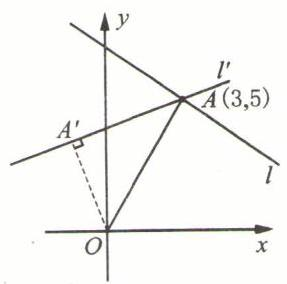
\includegraphics[width=0.2\textwidth]{bodyxb/src/bo_d20cdrf7aajc73bfmvhg_30_1239_1841_287_284_0.jpg}
\end{center}


[第 49(4)题]

(3) $x - y + 5 = 0$ 提示:记点 $A\left( {1,2}\right) ,B\left( {-1,4}\right)$ ,点 $A$ 在直线 $l$ 上的射影为点 $B$ ,意味着 ${AB}$  $\bot  l$ ,且 $l$ 过点 $B.{k}_{AB} = \dfrac{4 - 2}{-1 - 1} =  - 1,\therefore {k}_{l} = \dfrac{-1}{{k}_{AB}} = 1,\therefore l : y - 4 = 1 \cdot  \left( {x + 1}\right)$ ,即 $l : x - y + 5 = 0.$

(4) ${3x} + {5y} - {34} = 0$ 提示:记点 $A\left( {3,5}\right)$ ,如图,过点 $A$ 作直线 ${OA}$ 的垂线 $l$ ,过点 $A$ 作任意直线 ${l}^{\prime }$ (不与 $l$ 重合)及原点在 ${l}^{\prime }$ 上的射影 ${A}^{\prime }$ . 考察 $\bigtriangleup {OA}{A}^{\prime }$ ,其中 $\angle O{A}^{\prime }A = {90}^{ \circ  }$ ,

$\therefore \angle {A}^{\prime }{AO} < {90}^{ \circ  }$ . 根据大角对大边, $\left| {OA}\right|  > \left| {O{A}^{\prime }}\right|$ . 特别地. $O$ 与 ${A}^{\prime }$ 重合时. $\left| {OA}\right|  >$

$\left| {O{A}^{\prime }}\right|  = 0$ 也成立. 由此可见, $l$ 即为所求. $\because {k}_{OA} = \dfrac{5 - 0}{3 - 0} = \dfrac{5}{3},\therefore {k}_{l} =  - \dfrac{1}{{k}_{OA}} =  - \dfrac{3}{5}$ ,

$\therefore l : y - 5 =  - \dfrac{3}{5}\left( {x - 3}\right)$ ,即 $l : {3x} + {5y} - {34} = 0$ .

(5) $m =  - \dfrac{9}{8}$ 提示: 将 ${l}_{1} : \left( {2{m}^{2} + m - 3}\right) x + \left( {{m}^{2} - m}\right) y = {4m} - 1$ 转化为

$\left( {m - 1}\right) \left( {{2m} + 3}\right) x + m\left( {m - 1}\right) y = {4m} - 1$ . 若 $m\left( {m - 1}\right)  = 0$ ,即 ${m}_{1} = 0,{m}_{2} = 1$ . 当 $m = 0$ 时, ${l}_{1} :  - {3x} =  - 1$ ,与直线 ${l}_{2}$ : ${2x} - {3y} = 5$ 有交点 $\left( {\dfrac{1}{3}, - \dfrac{13}{9}}\right)$ . 当 $m = 1$ 时, ${l}_{1} : 0 = 3$ ,矛盾, $\therefore m\left( {m - 1}\right)  \neq  0$ ,即 $m \neq  0$ 且 $m \neq  1$ . 此时,将 ${l}_{1}$ 写成 $y =  - \dfrac{{2m} + 3}{m}x + \dfrac{{4m} - 1}{{m}^{2} - m}$ . 由题意, $- \dfrac{{2m} + 3}{m} = \dfrac{2}{3},\;\therefore \;m =  - \dfrac{9}{8}$ . 此时 ${l}_{1} : y = \dfrac{2}{3}x - \dfrac{352}{153},{l}_{2} : y = \dfrac{2}{3}x - \dfrac{5}{3}\;\therefore \;m$  $=  - \dfrac{9}{8}$ 时, ${l}_{1}//{l}_{2}$ .

(6) $m =  - 5$ 提示:直线 ${l}_{1} : {2x} - {5y} + {20} = 0$ 过点 $A\left( {0,4}\right)$ 和 $B\left( {-{10},0}\right)$ ,直线 ${l}_{2} : {mx} -$  ${2y} - {10} = 0$ 可转化为 $l : y = \dfrac{m}{2}x - 5$ ,过点 $C\left( {0, - 5}\right)$ 并交 $x$ 轴于 $E$ (如图),如图. ${l}_{1}$ 过第一、二、三象限, ${l}_{1},{l}_{2}$ 的交点为 $D$ ,也一定落在第一、二、三象限 (或坐标轴上).

\begin{center}
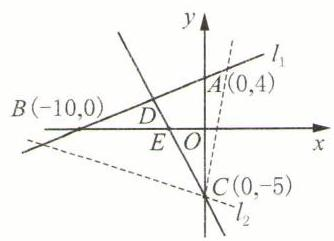
\includegraphics[width=0.2\textwidth]{bodyxb/src/bo_d20cdrf7aajc73bfmvhg_31_1085_603_334_241_0.jpg}
\end{center}


[第 49(6)题]

$\because {l}_{1},{l}_{2},x$ 轴, $y$ 轴围成的四边形有一个外接圆,而 $O,D$ 又是四边形两个相对的顶点, $\therefore {l}_{2} \bot  {l}_{1},\therefore {k}_{1} \cdot  {k}_{2} = \dfrac{2}{5} \cdot  \dfrac{m}{2} =  - 1$ . $\therefore m =  - 5$ . 此时 ${l}_{2} : y =  - \dfrac{5}{2}x - 5$ .

(7) ${3x} + {2y} - {3a} - {2b} = 0$ 提示:由题意, $l$ 过点(-1,2)和(-4,0), ${k}_{l} = \dfrac{2 - 0}{-1 + 4} = \dfrac{2}{3}$ . 记所求直线为 ${l}^{\prime }$ ,

$\therefore \;{l}^{\prime } : y - b =  - \dfrac{3}{2}\left( {x - a}\right)$ ,即 ${l}^{\prime } : {3x} + {2y} - \left( {{3a} + {2b}}\right)  = 0$ .

50. D 提示:由题意 $a\left( {a - 1}\right)  + \left( {1 - a}\right) \left( {{2a} + 3}\right)  = 0,\;\therefore \;{a}_{1} = 1,{a}_{2} =  - 3$ .

51. D 提示: 直线 ${l}_{1} : {5x} + {4y} + {21} = 0$ 的斜率为 $- \dfrac{5}{4}$ ,故与其垂直的直线斜率为 $\dfrac{4}{5}$ . 设点 $A\left( {4,0}\right)$ 关于 ${l}_{1}$ 的对称点为 $B(p$ , $q),{AB}$ 所在直线 ${l}_{2}$ 的方程为 $y - 0 = \dfrac{4}{5}\left( {x - 4}\right)$ . 联立 $\left\{  \begin{array}{l} y = \dfrac{4}{5}\left( {x - 4}\right) , \\  {5x} + {4y} + {21} = 0, \end{array}\right.$ 解得 $\left\{  \begin{array}{l} x =  - 1, \\  y =  - 4. \end{array}\right. \left( {-1, - 4}\right)$ 是 ${AB}$ 的中点, $\therefore \left\{  {\begin{array}{l} \dfrac{4 + p}{2} =  - 1, \\  \dfrac{0 + q}{2} =  - 4, \end{array}\text{ 解得 }\left\{  {\begin{array}{l} p =  - 6, \\  q =  - 8. \end{array}\therefore B\left( {-6, - 8}\right) .}\right. }\right.$

52. (1) 当 $b = 0$ 时, ${l}_{1} : {ax} + {2a} = 0$ ,故此时 $a \neq  0.{l}_{1}$ 进一步写为 ${l}_{1} : x =  - 2$ ,显然 ${l}_{1}$ 与 $x + {2y} + 3 = 0$ 相交, $\;\therefore b \neq  0$ . 此时, ${l}_{1} : y =  - \dfrac{a}{b}x - \dfrac{2a}{b},{l}_{2} : y = \left( {1 - a}\right) x - b,{l}_{3} : x + {2y} + 3 = 0$ 的斜率为 $- \dfrac{1}{2},{l}_{1}//{l}_{3},{l}_{2}//{l}_{3},\;\therefore \left\{  \begin{array}{l}  - \dfrac{a}{b} =  - \dfrac{1}{2}, \\  1 - a =  - \dfrac{1}{2}, \end{array}\right.$ 解得 $\left\{  \begin{array}{l} a = \dfrac{3}{2}, \\  b = 3. \end{array}\right.$ 此时, ${l}_{1} : x + {2y} + 2 = 0,{l}_{2} : x + {2y} + 6 = 0$ . 满足 ${l}_{1}//{l}_{3},{l}_{2}//{l}_{3}$ .

(2) ${l}_{1} \bot  {l}_{2}$ ,且 ${l}_{1}$ 过点 $\left( {-1,1}\right) ,\therefore \left\{  \begin{array}{l} a\left( {a - 1}\right)  + b = 0, \\   - a + b + {2a} = 0, \end{array}\right.$ 解得 $\left\{  \begin{array}{l} a = 0, \\  b = 0, \end{array}\right.$ 或 $\left\{  \begin{array}{l} a = 2, \\  b =  - 2. \end{array}\right.$ 当 $a = 0,b = 0$ 时, ${l}_{1} : 0 = 0$ 是恒等式,不是直线方程,舍去. 当 $a = 2,b =  - 2$ 时, ${l}_{1} : x - y + 2 = 0,{l}_{2} : x + y - 2 = 0$ 满足题意, $\therefore a = 2,b =  - 2$ .

53. (1) 先求出点 $C$ 的坐标. $\because {k}_{AB} = \dfrac{6 - 3}{6 - 2} = \dfrac{3}{4},{BC}\bot {AB},\therefore {k}_{AB} \cdot  {k}_{BC} =  - 1,{k}_{BC} =  - \dfrac{4}{3} = {k}_{AD}.\therefore {l}_{BC} : y - 6 =$  $- \dfrac{4}{3}\left( {x - 6}\right)$ . 可以通过 $\left| {BC}\right|  = \left| {AB}\right|$ 得到另一条直线方程求点 $C$ 的坐标,也可以通过求出 ${l}_{AC}$ 的方程求点 $C$ 的坐标. 以下是后面一种思路的解法,直线 ${AD}$ 的倾斜角 ${\alpha }_{AD}$ 和直线 ${AC}$ 的倾斜角 ${\alpha }_{AC}$ 有如下关系: ${\alpha }_{AD} + \dfrac{\pi }{4} = {\alpha }_{AC}$ ,

$\therefore {k}_{AC} = \tan {\alpha }_{AC} = \tan \left( {{\alpha }_{AD} + \dfrac{\pi }{4}}\right)  = \dfrac{\tan {\alpha }_{AD} + 1}{1 - \tan {\alpha }_{AD} \cdot  1} = \dfrac{{k}_{AD} + 1}{1 - {k}_{AD}} =  - \dfrac{1}{7},\;\therefore \;{l}_{AC} : y - 3 =  - \dfrac{1}{7}\left( {x - 2}\right)$ . 联立 $\left\{  {\begin{array}{l} {l}_{BC} : y - 6 =  - \dfrac{4}{3}\left( {x - 6}\right) , \\  {l}_{AC} : y - 3 =  - \dfrac{1}{7}\left( {x - 2}\right) , \end{array}\text{ 解得 }\left\{  \begin{array}{l} x = 9, \\  y = 2. \end{array}\right. }\right.$  $\therefore C\left( {9,2}\right) .\vv{BA} = \left( {2,3}\right)  - \left( {6,6}\right)  = \left( {-4, - 3}\right)  = \vv{CD},\therefore D\left( {5, - 1}\right)$ . 顶点 $C,D$ 的坐标为 $C\left( {9,2}\right) ,D\left( {5, - 1}\right)$ . (2) ${AB}$ 的中点为 $M\left( {\dfrac{a + 2 + b - 4}{2},\dfrac{b + 2 + a - b}{2}}\right)$ ,即 $M\left( {\dfrac{a + b - 2}{2},\dfrac{a + 2}{2}}\right)$ ,在 $l : {4x} + {3y} + {11} = 0$ 上, ${k}_{l} =  - \dfrac{4}{3}$ . 而 $l\bot {AB},\therefore {k}_{AB} = \dfrac{3}{4},{k}_{AB} = \dfrac{a - b - b - 2}{b - 4 - a - 2} = \dfrac{a - {2b} - 2}{-a + b - 6} = \dfrac{3}{4}$ . 联立 $\left\{  \begin{array}{l} 4 \cdot  \dfrac{a + b - 2}{2} + 3 \cdot  \dfrac{a + 2}{2} + {11} = 0, \\  \dfrac{a - {2b} - 2}{-a + b - 6} = \dfrac{3}{4}\left( {-a + b - 6 \neq  0}\right) , \end{array}\right.$ 解得 $\left\{  \begin{array}{l} a =  - \dfrac{52}{21}, \\  b =  - \dfrac{2}{3}. \end{array}\right.$ (3) 先求 $P\left( {-1,3}\right)$ 关于直线 $l : x + y + 1 = 0$ 对称的点 ${P}^{\prime }\left( {m,n}\right) .\because {k}_{l} =  - 1$ 且 $P{P}^{\prime }\bot l,\therefore {k}_{P{P}^{\prime }} =  - \dfrac{1}{{k}_{l}} = 1$ , $\therefore {l}_{P{P}^{\prime }} : y - 3 = 1 \cdot  \left( {x + 1}\right)$ . 联立 $\left\{  \begin{array}{l} y - 3 = x + 1, \\  x + y + 1 = 0, \end{array}\right.$ 解得 $\left\{  \begin{array}{l} x =  - \dfrac{5}{2}, \\  y = \dfrac{3}{2}. \end{array}\right. \left( {-\dfrac{5}{2},\dfrac{3}{2}}\right)$ 为线段 $P{P}^{\prime }$ 的中点, $\therefore \left\{  \begin{array}{l} \dfrac{-1 + m}{2} =  - \dfrac{5}{2}, \\  \dfrac{3 + n}{2} = \dfrac{3}{2}, \end{array}\right.$ 解得 $\left\{  \begin{array}{l} m =  - 4, \\  n = 0. \end{array}\right. \therefore {P}^{\prime }\left( {-4,0}\right)$ ,反射光线所在直线即 ${P}^{\prime }Q.{l}_{{P}^{\prime }Q} = \dfrac{y - 0}{-2 - 0} = \dfrac{x + 4}{4 - \left( {-4}\right) }$ ,即 ${l}_{{P}^{\prime }Q} : x + {4y} + 4 = 0.$

(4)在直线 $l : {3x} - {4y} + 4 = 0$ 中,代入 ${x}_{A} =  - 3$ ,则 $y =  - \dfrac{5}{4} < {y}_{A} = 5$ ,故点 $A$ 在直线 $l$ 的上方. 代入 ${x}_{B} = 2$ ,则 $y = \dfrac{5}{2} <$  ${y}_{B} = {15}$ ,故点 $B$ 也在直线 $l$ 的上方, $\therefore A,B$ 在直线 $l$ 同侧. 设点 $A$ 关于直线 $l$ 对称的点 ${A}^{\prime }\left( {m,n}\right)$ .

$\because \;{k}_{l} = \dfrac{3}{4}$ ,且 $A{A}^{\prime } \bot  l,\;\therefore \;{k}_{A{A}^{\prime }} =  - \dfrac{4}{3}$ .

$\therefore {l}_{A{A}^{\prime }} : y - 5 =  - \dfrac{4}{3}\left( {x + 3}\right)$ . 联立 $\left\{  \begin{array}{l} y - 5 =  - \dfrac{4}{3}\left( {x + 3}\right) , \\  {3x} - {4y} + 4 = 0, \end{array}\right.$ 解得 $\left\{  \begin{array}{l} x = 0, \\  y = 1. \end{array}\right. \left( {0,1}\right)$ 为线段 $A{A}^{\prime }$ 的中点,

$\therefore \left\{  {\begin{array}{l} \dfrac{-3 + m}{2} = 0, \\  \dfrac{5 + n}{2} = 1, \end{array}\text{ 解得 }\left\{  {\begin{array}{l} m = 3, \\  n =  - 3. \end{array}\;\therefore \;{A}^{\prime }\left( {3, - 3}\right) \text{ ,点 }{A}^{\prime }\text{ 与点 }B\text{ 在直线 }l\text{ 的两侧. }}\right. }\right.$

$\left| {PA}\right|  + \left| {PB}\right|  = \left| {P{A}^{\prime }}\right|  + \left| {PB}\right|  \geq  \left| {{A}^{\prime }B}\right|  = \sqrt{{1}^{2} + {18}^{2}} = 5\sqrt{13}$ ,当且仅当 $P$ 为 ${A}^{\prime }B$ 与 $l$ 的交点时,等号成立, $\left\{  {\begin{array}{l} {l}_{{A}^{\prime }B} : \dfrac{y + 3}{{15} - \left( {-3}\right) } = \dfrac{x - 3}{2 - 3}, \\  l : {3x} - {4y} + 4 = 0, \end{array}\text{ 解得 }\left\{  {\begin{array}{l} x = \dfrac{8}{3}, \\  y = 3. \end{array}\;\therefore \text{ 当 }P\text{ 取 }P\left( {\dfrac{8}{3},3}\right) \text{ 时,有 }\left| {PA}\right|  + \left| {PB}\right| }\right. }\right.$ 的最小值为 $5\sqrt{13}.$

(5) 对于直线 $l : {3x} - y - 1 = 0$ . 代入 ${x}_{A} = 4$ ,求得 $y = {11} > {y}_{A} = 1$ ,即点 $A$ 在 $l$ 下方,代入 ${x}_{B} = 0$ ,求得 $y =  - 1 < {y}_{B} = 4$ ,即点 $B$ 在 $l$ 上方, $\therefore A,B$ 在直线 $l$ 的两侧. 记 $B$ 点关于直线 $l$ 对称的点为 ${B}^{\prime }\left( {m,n}\right) ,\because {k}_{l} = 3,B{B}^{\prime }\bot l$ ,

$\therefore {k}_{B{B}^{\prime }} =  - \dfrac{1}{{k}_{1}} =  - \dfrac{1}{3},\;\therefore \;{l}_{B{B}^{\prime }} : y - 4 =  - \dfrac{1}{3}\left( {x - 0}\right)$ . 联立 $\left\{  \begin{array}{l} y - 4 =  - \dfrac{1}{3}x, \\  {3x} - y - 1 = 0, \end{array}\right.$ 解得 $\left\{  \begin{array}{l} x = \dfrac{3}{2}, \\  y = \dfrac{7}{2}. \end{array}\right. \left( {\dfrac{3}{2},\dfrac{7}{2}}\right)$ 即线段 $B{B}^{\prime }$ 的中点, $\therefore \left\{  \begin{array}{l} \dfrac{0 + m}{2} = \dfrac{3}{2}, \\  \dfrac{4 + n}{2} = \dfrac{7}{2}, \end{array}\right.$ 解得 $\left\{  \begin{array}{l} m = 3, \\  n = 3. \end{array}\right.$

即 ${B}^{\prime }\left( {3,3}\right) ,A{B}^{\prime }$ 在 $l$ 同侧. $\left| \right| {MA}\left| -\right| {MB}\left| \right|  = \left| \right| {MA}\left| -\right| M{B}^{\prime }\left| \right|  \leq  \left| {A{B}^{\prime }}\right|  = \sqrt{{1}^{2} + {2}^{2}} = \sqrt{5}$ . 当且仅当 $M$ 取直线 $A{B}^{\prime }$ 与直线 $l$ 的交点时,等号成立. $\left\{  \begin{array}{l} {l}_{A{B}^{\prime }} : \dfrac{y - 3}{1 - 3} = \dfrac{x - 3}{4 - 3}, \\  l : {3x} - y - 1 = 0, \end{array}\right.$ 解得 $\left\{  {\begin{array}{l} x = 2, \\  y = 5. \end{array}\;\therefore \;M\text{ 取 }M\left( {2,5}\right) }\right.$ 时, ${MA}$ 和 ${MB}$ 的距离之差的绝对值最大,为 $\sqrt{5}$ .

\begin{center}
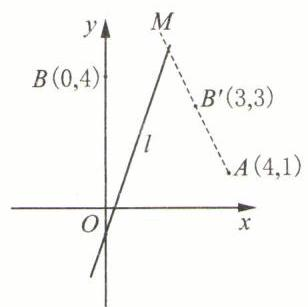
\includegraphics[width=0.2\textwidth]{bodyxb/src/bo_d20cdrf7aajc73bfmvhg_33_464_131_308_307_0.jpg}
\end{center}


[第 53(5)题]

\begin{center}
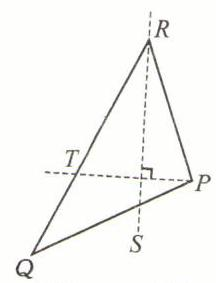
\includegraphics[width=0.2\textwidth]{bodyxb/src/bo_d20cdrf7aajc73bfmvhg_33_850_158_216_283_0.jpg}
\end{center}


[第 53(6)题]

(6)记内角 $B,C$ 的平分线分别为 ${l}_{B},{l}_{C}$ . 如图,对任意 $\bigtriangleup {PQR}$ ,内角 $R$ 的平分线为 ${RS}$ ,过 $P$ 作 ${RS}$ 的垂线交 ${RQ}$ 于点 $T$ , 容易证明 ${RS}$ 垂直平分线段 ${PT}$ ,故 $T$ 是点 $P$ 关于直线 ${RS}$ 对称的点. 由此可见,若求得点 $A$ 关于 ${l}_{B},{l}_{C}$ 对称的点 ${A}_{2},{A}_{3}$ ,则点 ${A}_{2},{A}_{3}$ 均在直线 ${BC}$ 上. 下面先求点 ${A}_{2}$ .

$\because {l}_{B} : y = x - 1,{k}_{B} = 1,A{A}_{2} \bot  {l}_{B},\;\therefore \;{k}_{A{A}_{2}} =  - \dfrac{1}{{k}_{B}} =  - 1,{l}_{A{A}_{2}} : y + 1 =  - \left( {x - 4}\right)$ . 联立 $\left\{  \begin{array}{l} y + 1 =  - \left( {x - 4}\right) , \\  y = x - 1, \end{array}\right.$ 解得 $\left\{  {\begin{array}{l} x = 2, \\  y = 1. \end{array}\left( {2,1}\right) }\right.$ 即为 $A{A}_{2}$ 的中点,已知 $A\left( {4, - 1}\right)$ ,易知 ${A}_{2}\left( {0,3}\right)$ . 再求点 ${A}_{3}$ .

$\because {l}_{3} : x = 1,{l}_{3} \bot  x$ 轴,不难看出 ${A}_{3}$ 的坐标是 $\left( {1 \times  2 - 4, - 1}\right)$ ,即 ${A}_{3}\left( {-2, - 1}\right)$ .

$\therefore \;{l}_{BC} : \dfrac{y - 3}{-1 - 3} = \dfrac{x - 0}{-2 - 0}$ ,即 ${l}_{BC} : {2x} - y + 3 = 0$ .

54. 由题意,两条直线的斜率之积为 $- 1,\lg \left( {ac}\right)  \cdot  \lg \left( {bc}\right)  =  - 1.\;\therefore \;\left( {\lg c + \lg a}\right) \left( {\lg c + \lg b}\right)  =  - 1$ . 记 $t = \lg c \in  \mathbf{R}\;\therefore \;{t}^{2} +$  $\left( {\lg a + \lg b}\right) t + \lg a \cdot  \lg b =  - 1$ . 该方程有实数解. $\therefore \Delta  = {\left( \lg a + \lg b\right) }^{2} - 4\left( {\lg a \cdot  \lg b + 1}\right)  = {\left( \lg a - \lg b\right) }^{2} - 4 \geq  0$ ,

$\therefore \;{\left( \lg \dfrac{a}{b}\right) }^{2} \geq  4.\;\therefore \;\lg \dfrac{a}{b} \geq  2$ 或 $\lg \dfrac{a}{b} \leq   - 2,$

$\therefore \dfrac{a}{b} \geq  {10}^{2}$ 或 $0 < \dfrac{a}{b} \leq  {10}^{-2},\therefore \dfrac{a}{b}$ 的取值范围为 $\dfrac{a}{b} \geq  {100}$ 或 $0 < \dfrac{a}{b} \leq  \dfrac{1}{100}$ .

55. A 提示: 方法一: ${k}_{1} = \sqrt{3},{k}_{2} = \dfrac{\sqrt{3}}{3}$ ,设 ${l}_{1}$ 到 ${l}_{2}$ 的角为 $\theta \tan \theta  = \dfrac{{k}_{2} - {k}_{1}}{1 + {k}_{1}{k}_{2}} = \dfrac{\dfrac{\sqrt{3}}{3} - \sqrt{3}}{1 + 1} =  - \dfrac{\sqrt{3}}{3}$ .

$\therefore \theta  = \arctan \left( {-\dfrac{\sqrt{3}}{3}}\right)  + \pi  = \pi  - \dfrac{\pi }{6} = \dfrac{5}{6}\pi$ .

方法二: 由 ${k}_{1} = \sqrt{3},{k}_{2} = \dfrac{\sqrt{3}}{3}$ ,易知: ${\alpha }_{1} = {60}^{ \circ  },{\alpha }_{2} = {30}^{ \circ  },{l}_{1}$ 逆时钟旋转 ${180}^{ \circ  } - \left( {{60}^{ \circ  } - {30}^{ \circ  }}\right)  = {150}^{ \circ  }$ 方能与 ${l}_{2}$ 重合.

56. D 提示: 记 ${l}_{1},{l}_{2}$ 的斜率分别为 ${k}_{1},{k}_{2}$ ,则 ${k}_{1} = \dfrac{1}{2}$ . 由题意, $\dfrac{{k}_{2} - {k}_{1}}{1 + {k}_{1}{k}_{2}} = \dfrac{{k}_{2} - \dfrac{1}{2}}{1 + \dfrac{1}{2}{k}_{2}} = \tan {45}^{ \circ  } = 1,\therefore {k}_{2} = 3$ .

$\therefore \;{l}_{2} : y - 1 = 3\left( {x + 2}\right)$ ,即 ${l}_{2} : y = {3x} + 7$ .

57. $C$ 提示: 设直线 $l$ 的斜率为 $k$ ,直线 ${2x} + y - 1 = 0$ 的斜率为 -2. 由题意, $\left| \dfrac{k - \left( {-2}\right) }{1 + \left( {-2}\right) k}\right|  = \tan {45}^{ \circ  } = 1$ ,解得 $k =  - \dfrac{1}{3}$ 或 $k$  $= 3$ .

58. B 提示: 由题意, ${k}_{1} + {k}_{2} =  - \dfrac{1}{6},{k}_{1}{k}_{2} =  - \dfrac{1}{6}\left( {\Delta  > 0}\right) ,\therefore {l}_{1}$ 与 ${l}_{2}$ 的夹角 $\theta$ 满足: $\tan \theta  = \left| \dfrac{{k}_{1} - {k}_{2}}{1 + {k}_{1}{k}_{2}}\right|  =$  $\dfrac{\sqrt{{\left( {k}_{1} + {k}_{2}\right) }^{2} - 4{k}_{1}{k}_{2}}}{\left| 1 + {k}_{1}{k}_{2}\right| } = \dfrac{\sqrt{\dfrac{1}{36} + \dfrac{2}{3}}}{\dfrac{5}{6}} = 1.\;\therefore \;\theta  = \arctan 1 = {45}^{ \circ  }.$

59. (1) $\dfrac{\pi }{2} - \arctan \dfrac{1}{2}$ 提示:直线 ${l}_{1} : x + 1 = 0$ 的斜率不存在,故不能使用夹角公式. ${l}_{1}$ 的倾斜角为 ${\alpha }_{1} = \dfrac{\pi }{2}$ . 直线 ${l}_{2} : x + {2y}$  $- 3 = 0$ ,斜率为 $- \dfrac{1}{2}$ ,故 ${l}_{2}$ 的倾斜角为: ${\alpha }_{2} = \arctan \left( {-\dfrac{1}{2}}\right)  + \pi  = \pi  - \arctan \dfrac{1}{2}.{l}_{1}$ 与 ${l}_{2}$ 的夹角 $\theta  = \left| {{\alpha }_{1} - {\alpha }_{2}}\right|  = \dfrac{\pi }{2} -$  $\arctan \dfrac{1}{2}$

(2) $\dfrac{5}{18}\pi$ 提示:原二次方程可写为 $\left( {x + \sqrt{3}}\right) \left( {x - 1}\right)  = 0$ .

$\therefore {x}_{1} =  - \sqrt{3},{x}_{2} = 1.{l}_{1}$ 与 ${l}_{2}$ 的夹角为 $\left| {\arctan \left( {-\sqrt{3}}\right)  + \pi  - \arctan 1}\right|  = \left| {\pi  - \dfrac{\pi }{3} - \dfrac{\pi }{4}}\right|  = \dfrac{5}{12}\pi$ .

(3) $m = \dfrac{1}{3}$ 或 $m =  - 3$ 提示:直线 ${2x} - y = 0$ 的斜率为 2,直线 ${mx} - y = 0$ 的斜率为 $m$ . 由题意: $\left| \dfrac{m - 2}{1 + {2m}}\right|  = \tan {45}^{ \circ  } = 1$ . $\therefore m =  - 3$ 或 $m = \dfrac{1}{3}$ .

(4) ${3x} + y + 6 = 0$ 或 $\dfrac{1}{3}x - y + \dfrac{2}{3} = 0$ 提示: 直线 ${l}_{1} : {2x} - y + 4 = 0$ 的斜率为 ${k}_{1} = 2,{l}_{1}$ 与 $x$ 轴交于点(-2,0),设所求直线为 ${l}_{2}$ ,斜率为 ${k}_{2}$ . 由题意: $\left| \dfrac{{k}_{2} - 2}{1 + 2{k}_{2}}\right|  = \tan {45}^{ \circ  } = 1,\therefore {k}_{2} =  - 3$ 或 ${k}_{2} = \dfrac{1}{3}$ .

$\therefore \;{l}_{2} : y - 0 =  - 3\left( {x + 2}\right)$ 或 $y - 0 = \dfrac{1}{3}\left( {x + 2}\right)$ ,即 ${3x} + y + 6 = 0$ 或 $x - {3y} + 2 = 0$ .

60. C 提示: 设题中三条直线分别为 ${l}_{1},{l}_{2},{l}_{3}$ . 易知三者斜率为 ${k}_{1} = \dfrac{3}{4},{k}_{2} =  - \dfrac{4}{3},{k}_{3} = 7.\;\because {k}_{1} \cdot  {k}_{2} =  - 1,\therefore {l}_{1} \bot  {l}_{2}$ . ${l}_{1},{l}_{3}$ 之间的夹角为 ${\theta }_{13}$ ,则 $\tan {\theta }_{13} = \left| \dfrac{{k}_{1} - {k}_{3}}{1 + {k}_{1}{k}_{3}}\right|  = \left| \dfrac{\dfrac{3}{4} - 7}{1 + \dfrac{3}{4} \cdot  7}\right|  = 1.\;\therefore \;{\theta }_{13} = \dfrac{\pi }{4}$ . 因此 ${l}_{1},{l}_{2},{l}_{3}$ 所围成的三角形中,三个内角为 ${90}^{ \circ  },{45}^{ \circ  },{45}^{ \circ  }\left( {{180}^{ \circ  } - {90}^{ \circ  } - {45}^{ \circ  } = {45}^{ \circ  }}\right)$ ,故为等腰直角三角形.

61. A 提示: 斜边 ${AB}$ 所在直线为 ${3x} - y + 2 = 0$ ,其斜率为 ${k}_{AB} = 3,{AC}$ 与 ${AB},{BC}$ 与 ${AB}$ 的夹角都是 ${45}^{ \circ  }$ ,它们的斜率满足以下关于 $k$ 的方程: $\left| \dfrac{k - {k}_{AB}}{1 + k \cdot  {k}_{AB}}\right|  = \left| \dfrac{k - 3}{1 + {3k}}\right|  = \tan {45}^{ \circ  } = 1,\therefore k = \dfrac{1}{2}$ 或 $k =  - 2$ . 利用点斜式可写出 ${AC}$ 与 ${BC}$ 的方程 (不分先后): $y + 2 = \dfrac{1}{2}\left( {x - 3}\right) ,y + 2 =  - 2\left( {x - 3}\right)$ ,即 $x - {2y} - 7 = 0,{2x} + y - 4 = 0$ .

62. (1) ${3x} + {7y} - {13} = 0$ 或 ${7x} - {3y} - {11} = 0$ 提示: 记 ${l}_{1},{l}_{2}$ 的斜率分别为 ${k}_{1},{k}_{2}$ ,易知 ${k}_{1} =  - \dfrac{5}{2},{k}_{2}$ 满足: $\left| \dfrac{{k}_{2} - {k}_{1}}{1 + {k}_{1}{k}_{2}}\right|  =$  $\left| \dfrac{{k}_{2} + \dfrac{5}{2}}{1 - \dfrac{5}{2}{k}_{2}}\right|  = \tan {45}^{ \circ  } = 1.\;\therefore \;{k}_{2} =  - \dfrac{3}{7}$ 或 ${k}_{2} = \dfrac{7}{3}.{k}_{2} =  - \dfrac{3}{7}$ 时, ${l}_{2} : y - 1 =  - \dfrac{3}{7}\left( {x - 2}\right)$ ,即 ${3x} + {7y} - {13} = 0.{k}_{2} = \dfrac{7}{3}$ 时, ${l}_{2} : y - 1 = \dfrac{7}{3}\left( {x - 2}\right)$ ,即 ${7x} - {3y} - {11} = 0.\;\therefore$ 直线 ${l}_{2}$ 的方程为 ${3x} + {7y} - {13} = 0$ 或 ${7x} - {3y} - {11} = 0$ .

(2) ${2x} - {6y} - 3 = 0$ 提示:直线 ${l}_{1} : x + {2y} + 1 = 0$ 与 $y$ 轴交于点 $\left( {0, - \dfrac{1}{2}}\right)$ ,斜率 ${k}_{1} =  - \dfrac{1}{2}$ . 设直线 $l$ 的斜率为 $k$ . 由题意, $l$ 到 $l$ 的角为 $\dfrac{\pi }{4}$ . $\therefore \dfrac{k - {k}_{1}}{1 + k{k}_{1}} = \dfrac{k + \dfrac{1}{2}}{1 - \dfrac{1}{2}k} = \tan \dfrac{\pi }{4} = 1,\therefore k = \dfrac{1}{3},\therefore l : y + \dfrac{1}{2} = \dfrac{1}{3}\left( {x - 0}\right)$ ,即 $l : {2x} - {6y} - 3$  $= 0$ .

63. (1) 底边 ${BC}$ 所在直线的斜率为 ${k}_{BC} =  - 1$ . 不妨设 ${AB}$ 与 $x - {4y} + 2 = 0$ 平行,故 ${k}_{AB} = \dfrac{1}{4}$ . $\because \bigtriangleup {ABC}$ 是等腰三角形且 $A$ 为顶点 $\therefore \left| \dfrac{{k}_{BC} - {k}_{AB}}{1 + {k}_{BC} \cdot  {k}_{AB}}\right|  = \left| \dfrac{{k}_{BC} - {k}_{AC}}{1 + {k}_{BC} \cdot  {k}_{AC}}\right| ,\;\therefore \left| \dfrac{-1 - \dfrac{1}{4}}{-1 + \dfrac{1}{4}}\right|  = \left| \dfrac{-1 - {k}_{AC}}{-1 + {k}_{AC}}\right|$ , $\therefore {k}_{AC} = 4\left( {{k}_{AC} = \dfrac{1}{4}\text{ 舍去 }}\right) .\;\therefore$ 另一腰 ${AC}$ 所在直线为 $y - 3 = 4\left( {x - 2}\right)$ ,即 ${4x} - y - 5 = 0.$

(2)两腰所在直线 ${l}_{1} : x + y - 2 = 0$ 和 ${l}_{2} : {7x} - y + 4 = 0$ 的斜率分别为 ${k}_{1} =  - 1,{k}_{2} = 7$ ,两直线的交点为 $\left( {-\dfrac{1}{4},\dfrac{9}{4}}\right)$ . 若底边 ${l}_{3}$ 垂直于 $x$ 轴,则易知 ${l}_{1},{l}_{3}$ 之间的夹角为 ${45}^{ \circ  }$ . 而 ${l}_{2},{l}_{3}$ 的夹角明显不是 ${45}^{ \circ  }$ .

$\therefore$ 底边不可能垂直于 $x$ 轴,故 ${l}_{3}$ 的斜率存在,记为 ${k}_{3}.\therefore {l}_{3}$ 与 ${l}_{1}$ 的夹角和 ${l}_{3}$ 与 ${l}_{2}$ 的夹角相等.

$\therefore \left| \dfrac{{k}_{3} - {k}_{1}}{1 + {k}_{1}{k}_{3}}\right|  = \left| \dfrac{{k}_{3} - {k}_{2}}{1 + {k}_{2}{k}_{3}}\right| ,\;\therefore \;\left| \dfrac{{k}_{3} + 1}{1 - {k}_{3}}\right|  = \left| \dfrac{{k}_{3} - 7}{1 + 7{k}_{3}}\right| ,\;\therefore \;\left| {7{k}_{3} + 1}\right|  \cdot  \left| {{k}_{3} + 1}\right|  = \left| {{k}_{3} - 7}\right|  \cdot  \left| {{k}_{3} - 1}\right|$ ,即 $\mid  7{k}_{3}^{2}$  $+ 8{k}_{3} + 1\left|  = \right| {k}_{3}^{2} - 8{k}_{3} + 7\left| {\text{ . 当 }7{k}_{3}^{2} + 8{k}_{3} + 1 =  - \left( {{k}_{3}^{2} - 8{k}_{3} + 7}\right) }\right|$ 时,无实数根. $\therefore 7{k}_{3}^{2} + 8{k}_{3} + 1 = {k}_{3}^{2} - 8{k}_{3} + 7$ ,可得 ${k}_{3}$  $= \dfrac{1}{3}$ 或 ${k}_{3} =  - 3$ . 当 ${k}_{3} = \dfrac{1}{3}$ 时, ${l}_{3} : y - 1 = \dfrac{1}{3}\left( {x - 2}\right)$ ,即 $x - {3y} + 1 = 0$ . 当 ${k}_{3} =  - 3$ 时, ${l}_{3} : y - 1 =  - 3\left( {x - 2}\right)$ ,即 ${3x} + y$  $- 7 = 0$ . 经验证可知, ${l}_{1},{l}_{2}$ 的交点 $\left( {-\dfrac{1}{4},\dfrac{9}{4}}\right)$ 均不在 ${l}_{3}$ 上 $\therefore$ 底边所在直线的方程为 $x - {3y} + 1 = 0$ 或 ${3x} + y - 7$  $= 0$ .

64. B 提示: 联立 $\left\{  \begin{array}{l} {2x} + {3y} + 8 = 0, \\  x - y - 1 = 0, \end{array}\right.$ 解得 $\left\{  \begin{array}{l} x =  - 1, \\  y =  - 2. \end{array}\right.$ 将(-1, - 2)代入 $x + {ky} = 0$ ,得 $- 1 - {2k} = 0$ .

$\therefore k =  - \dfrac{1}{2}$ .

65. D 提示: 联立 $\left\{  \begin{array}{l} {5x} + {4y} = {2m} + 1, \\  {2x} + {3y} = m, \end{array}\right.$ 解得 $\left\{  \begin{array}{l} x = \dfrac{{2m} + 3}{7}, \\  y = \dfrac{m - 2}{7}. \end{array}\right.$ 由题意 $\left\{  \begin{array}{l} x = \dfrac{{2m} + 3}{7} > 0, \\  y = \dfrac{m - 2}{7} < 0, \end{array}\right.$ 得 $- \dfrac{3}{2} < m < 2$ .

66. C 提示:对于(A):两直线斜率相等,除两直线平行外,也可以重合,错误. 对于(B):若 ${l}_{1}//{l}_{2}//y$ 轴,此时 ${l}_{1},{l}_{2}$ 的斜率均不存在,错误. 对于(C): 这两条直线可以写成 $y = {kx} + b$ 和 $x = a$ 的形式必有交点 $\left( {a,{ak} + b}\right)$ ,故 ${l}_{1}$ 与 ${l}_{2}$ 一定相交,正确. 对于 $\left( D\right)  : {l}_{1},{l}_{2}$ 的斜率都不存在时, ${l}_{1}//{l}_{2}$ 或 ${l}_{1}$ 与 ${l}_{2}$ 重合,错误.

67. $C$ 提示: 若 ${m}^{2} - m = 0$ ,即 ${m}_{1} = 0$ 或 ${m}_{2} = 1$ . 对于 ${m}_{1} = 0$ ,有 ${l}_{1} \mathrel{\text{ := }} {3x} =  - 1$ ,与 ${l}_{2}$ 有交点 $\left( {\dfrac{1}{3}, - \dfrac{13}{9}}\right)$ ; 对于 ${m}_{2} = 1$ ,有 ${l}_{1}$ ; $0 = 3$ ,矛盾. $\therefore {m}^{2} - m \neq  0$ ,此时有 ${l}_{1} : y =  - \dfrac{2{m}^{2} + m - 3}{{m}^{2} - m}x + \dfrac{{4m} - 1}{{m}^{2} - m} =  - \dfrac{{2m} + 3}{m}x + \dfrac{{4m} - 1}{{m}^{2} - m},{l}_{1}//{l}_{2} \Rightarrow  {k}_{1} =  - \dfrac{{2m} + 3}{m} =$  ${k}_{2} = \dfrac{2}{3},\;\therefore m =  - \dfrac{9}{8}$ . 此时 ${l}_{1} : {2x} - {3y} - \dfrac{352}{51} = 0,\;\therefore m =  - \dfrac{9}{8}$ 时, ${l}_{1}//{l}_{2}$ .

68. $C$ 提示:对于 ${l}_{1} : {3x} - {2y} + m = 0$ ,其斜率为 ${k}_{1} = \dfrac{3}{2}$ . 对于 ${l}_{2} : \left( {{m}^{2} + 1}\right) x + {3y} - {3m} = 0$ ,其斜率为 ${k}_{2} =  - \dfrac{{m}^{2} + 1}{3}$ .

$\because {k}_{2} < 0 < {k}_{1}\;\therefore \;{l}_{1}$ 与 ${l}_{2}$ 一定相交.

69. 当 $a + 3 = 0$ 即 $a =  - 3$ 时, ${l}_{1} \mathrel{\text{ := }} x = 5,{l}_{2} : {6x} - {7y} = 5,{l}_{1}$ 与 ${l}_{2}$ 相交于(-5, - 5); 当 ${2a} - 1 = 0$ ,即 $a = \dfrac{1}{2}$ 时, ${l}_{1} : \dfrac{5}{2}x + \dfrac{7}{2}y$  $= 5,{l}_{2} : {6x} = 5,{l}_{1}$ 与 ${l}_{2}$ 相交于 $\left( {\dfrac{5}{6},\dfrac{5}{6}}\right)$ ,故 ${l}_{1}$ 与 ${l}_{2}$ 重合或平行时, $a \neq   - 3$ 且 $a \neq  \dfrac{1}{2}$ . 此时 ${l}_{1} : y =  - \dfrac{a + 2}{a + 3}x + \dfrac{5}{a + 3},{l}_{2} : y$  $=  - \dfrac{6}{{2a} - 1}x + \dfrac{5}{{2a} - 1}.$

(1)4 提示: ${l}_{1}$ 与 ${l}_{2}$ 重合时,有 $\left\{  \begin{array}{l}  - \dfrac{a + 2}{a + 3} =  - \dfrac{6}{{2a} - 1}, \\  \dfrac{5}{a + 3} = \dfrac{5}{{2a} - 1}, \end{array}\right.$ 解得 $a = 4$ .

(2) $- \dfrac{5}{2}$ 提示: ${l}_{1}$ 与 ${l}_{2}$ 平行时,有 $\left\{  \begin{array}{l}  - \dfrac{a + 2}{a + 3} =  - \dfrac{6}{{2a} - 1}, \\  \dfrac{5}{a + 3} \neq  \dfrac{5}{{2a} - 1}, \end{array}\right.$ 解得 $a =  - \dfrac{5}{2}$ .

(3)-1或 $- \dfrac{9}{2}$ 提示: ${l}_{1}$ 与 ${l}_{2}$ 垂直时,有 $\left( {a + 2}\right)  \cdot  6 + \left( {a + 3}\right) \left( {{2a} - 1}\right)  = 0,\;\therefore a =  - 1$ 或 $a =  - \dfrac{9}{2}$ .

70. (1) $m = 5,n =  - {12},a =  - 2$ 提示: 由题意得 $\left\{  \begin{array}{l} {2m} - {10} = 0, \\  m + {2a} - 1 = 0, \\  2 - {5a} + n = 0, \end{array}\right.$ 解得 $\left\{  \begin{array}{l} m = 5, \\  n =  - {12}, \\  a =  - 2. \end{array}\right.$

(2) $a =  - 1,c = 1,m =  - \dfrac{1}{2}$ 提示: 记直线 ${l}_{1},{l}_{2}$ 的斜率分别为 ${k}_{1},{k}_{2}$ ,则 ${k}_{1} =  - \dfrac{a}{2},{k}_{2} =  - \dfrac{1}{3}$ . 记 ${l}_{2}$ 到 ${l}_{1}$ 的角为 $\theta$ ,则 $\tan \theta  = \dfrac{{k}_{1} - {k}_{2}}{1 + {k}_{1}{k}_{2}} = \dfrac{-\dfrac{a}{2} + \dfrac{1}{3}}{1 + \dfrac{a}{6}}$ ,联立 $\left\{  \begin{array}{l} \dfrac{-\dfrac{a}{2} + \dfrac{1}{3}}{1 + \dfrac{a}{6}} = \tan {45}^{ \circ  } = 1, \\  \dfrac{1}{1 + \dfrac{a}{6}} = 1, \\  a + {2m} + 2 = 0, \\  2 + {6m} + c = 0, \end{array}\right.$ 解得 $\left\{  \begin{array}{l} a =  - 1, \\  c = 1, \\  m =  - \dfrac{1}{2}. \end{array}\right.$ 71. A 提示: 直线 ${l}_{1} : x - \sqrt{3}y = 0$ 的斜率 ${k}_{1} = \dfrac{\sqrt{3}}{3}$ ,倾斜角 ${\alpha }_{1} = \dfrac{\pi }{6}$ . 直线 ${l}_{2} : x - 1 = 0$ 的斜率不存在,倾斜角 ${\alpha }_{2} = \dfrac{\pi }{2},{l}_{1},{l}_{2}$ 的夹角是 $\left| {\dfrac{\pi }{6} - \dfrac{\pi }{2}}\right|  = \dfrac{\pi }{3}$ . 夹角平分线 ${l}_{3}$ 的倾斜角为 ${\alpha }_{3} : \dfrac{\pi }{6} + \dfrac{1}{2} \cdot  \dfrac{\pi }{3} = \dfrac{\pi }{3},{k}_{3} = \tan {\alpha }_{3} = \sqrt{3}.{l}_{1},{l}_{2}$ 交于点 $\left( {1,\dfrac{\sqrt{3}}{3}}\right)$ ,

$\therefore \;{l}_{3} : y - \dfrac{\sqrt{3}}{3} = \sqrt{3}\left( {x - 1}\right)$ ,即 ${l}_{3} : {3x} - \sqrt{3}y - 2 = 0$ .

72. A 提示: 方法一: $x < 0$ 时, $y = a\left| x\right|  =  - {ax}$ ,与 $y = x + a$ 有且只有一个交点,交点满足 $\left\{  \begin{array}{l} y =  - {ax}, \\  y = x + a, \end{array}\right.$ 解得 $\left\{  \begin{array}{l} x =  - \dfrac{a}{a + 1}\left( {x < 0}\right) , \\  y = \dfrac{{a}^{2}}{a + 1}. \end{array}\right.$ 因此, $y = a\left| x\right|$ 与 $y = x + a$ 若有两个交点,则要求在 $x \geq  0$ 时, $y = a\left| x\right|  = {ax}$ 与 $y = x + a$ 有且只有一个交点. $\left\{  \begin{array}{l} y = {ax}, \\  y = x + a, \end{array}\right.$ 消去 $y$ ,得 $\left( {a - 1}\right) x = a.\because a > 0,\therefore a - 1 = 0$ 时以上方程为 $0 = a$ ,不成立. $\therefore a - 1 \neq  0$ , $x = \dfrac{a}{a - 1} > 0,\;\therefore \;a > 1$ .

方法二: $\left\{  \begin{array}{l} y = a\left| x\right| , \\  y = x + a, \end{array}\right.$ 消去 $y$ ,有 $a\left| x\right|  = x + a$ . 该方程等价于: $\left\{  \begin{array}{l} {a}^{2}{x}^{2} = {\left( x + a\right) }^{2}, \\  x + a \geq  0, \end{array}\right.$ 即 $\left\{  \begin{array}{l} \left( {1 - {a}^{2}}\right) {x}^{2} + {2ax} + {a}^{2} = 0, \\  x \geq   - a. \end{array}\right.$ 该方程有两组解, $\therefore a \neq  1$ ,此时 $\left( {1 - {a}^{2}}\right) {x}^{2} + {2ax} + {a}^{2} = 0$ 在 $x \geq   - a$ 上有两个不等实根. $\Delta  = 4{a}^{2} - 4\left( {1 - {a}^{2}}\right)  \cdot  {a}^{2} = 4{a}^{4} > 0$ . $\therefore {x}_{1,2} = \dfrac{-{2a} \pm  2{a}^{2}}{2\left( {1 - {a}^{2}}\right) } = \dfrac{-a \pm  {a}^{2}}{1 - {a}^{2}},{x}_{1,2} + a = \dfrac{-a \pm  {a}^{2} + a - {a}^{3}}{1 - {a}^{2}} = \dfrac{{a}^{3} \mp  {a}^{2}}{{a}^{2} - 1} = \dfrac{{a}^{2}\left( {a \mp  1}\right) }{\left( {a + 1}\right) \left( {a - 1}\right) } = \dfrac{{a}^{2}}{a \pm  1}$ .

$\because a > 0,\;\therefore \dfrac{{a}^{2}}{a + 1} > 0,\;\therefore {x}_{1,2} + a \geq  0 \Leftrightarrow  \dfrac{{a}^{2}}{a - 1} > 0 \Leftrightarrow  a > 1$ .

73. $C$ 提示:将直线方程 ${l}_{i} : {a}_{i}x + {b}_{i}y + 1 = 0$ 视为 ${l}_{i} : x \cdot  {a}_{i} + y \cdot  {b}_{i} + 1 = 0\left( {i = 1,2}\right) .P\left( {2,3}\right)$ 在 ${l}_{1},{l}_{2}$ 上,故 $2{a}_{i} + 3{b}_{i} + 1 = 0$  $\left( {i = 1,2}\right)$ . 容易看出 ${a}_{1} = {a}_{2}$ 时必有 ${b}_{1} = {b}_{2}$ ,故 ${Q}_{1},{Q}_{2}$ 是相异的两点时, ${a}_{1} \neq  {a}_{2}$ 且 ${b}_{1} \neq  {b}_{2}$ . 过 ${Q}_{1},{Q}_{2}$ 的直线唯一确定, 且满足 $2{a}_{i} + 3{b}_{i} + 1 = 0,\therefore$ 直线 ${Q}_{1}{Q}_{2}$ 的方程为 ${2x} + {3y} + 1 = 0$ .

74. (1) 先求 ${l}_{1} : {4x} + y - 4 = 0$ 与 ${l}_{2} : {mx} + y = 0$ 的交点, $\left( {m \neq  4\text{ ,否则 }{l}_{1}//{l}_{2}}\right) \left\{  \begin{array}{l} {4x} + y - 4 = 0, \\  {mx} + y = 0, \end{array}\right.$ 解得 $\left\{  \begin{array}{l} x = \dfrac{4}{4 - m}, \\  y =  - \dfrac{4m}{4 - m}. \end{array}\right. \left( {m \neq  4}\right)$ 将 $\left( {\dfrac{4}{4 - m}, - \dfrac{4m}{4 - m}}\right)$ 代入 ${l}_{3} : {2x} - {3my} - 4 = 0$ ,得 $2 \cdot  \dfrac{4}{4 - m} + \dfrac{{12}{m}^{2}}{4 - m} - 4 = 0$ ,解得 ${m}_{1} =  - 1,{m}_{2} = \dfrac{2}{3}$ 均满足 $m \neq  4$ . $\therefore m =  - 1$ 或 $m = \dfrac{2}{3}$ 时,三条直线相交于一点.

(2)除了(1)中情况之外,考虑有两直线平行的情况. 得 $m = 4$ 或 $m =  - \dfrac{1}{6}.\;\therefore \;m = 4$ 或 $m =  - \dfrac{1}{6}$ 或 $m =  - 1$ 或 $m =$  $\dfrac{2}{3}$ 时,这三条直线不能构成三角形.

75. 根据菱形性质, $\left| {BA}\right|  = \left| {BC}\right|$ ,故 ${AC}$ 的垂直平分线 ${l}_{2}$ 与 ${AB}$ 所在直线 ${l}_{1}$ 的交点即为 $B.{k}_{AC} = \dfrac{4 - 2}{4 - \left( {-2}\right) } = \dfrac{1}{3},{l}_{2}$ 的斜率 ${k}_{2} =  - \dfrac{1}{{k}_{AC}} =  - 3$ ,且过线段 ${AC}$ 的中点 $\left( {1,3}\right) ,\therefore {l}_{2} : y - 3 =  - 3\left( {x - 1}\right)$ ,即 ${l}_{2} : {3x} + y - 6 = 0$ . 联立 $\left\{  \begin{array}{l} x - y + 4 = 0, \\  {3x} + y - 6 = 0, \end{array}\right.$ 解得 $\left\{  {\begin{array}{l} x = \dfrac{1}{2}, \\  y = \dfrac{9}{2}. \end{array}\therefore B\left( {\dfrac{1}{2},\dfrac{9}{2}}\right) ,\vv{CD} = \vv{BA} = \left( {-2,2}\right)  - \left( {\dfrac{1}{2},\dfrac{9}{2}}\right)  = \left( {-\dfrac{5}{2}, - \dfrac{5}{2}}\right) }\right.$ . 已知 $C\left( {4,4}\right)$ ,得 $D\left( {\dfrac{3}{2},\dfrac{3}{2}}\right)$ 从而 ${CD}$ ,

${AD}$ , ${BC}$ 所在直线的方程: ${l}_{CD} : \dfrac{y - 4}{\dfrac{3}{2} - 4} = \dfrac{x - 4}{\dfrac{3}{2} - 4}$ ,即 ${l}_{CD} : x - y = 0,{l}_{AD} : \dfrac{y - 2}{\dfrac{3}{2} - 2} = \dfrac{x + 2}{\dfrac{3}{2} + 2}$ ,即 ${l}_{AD} : x + {7y} - {12} = 0,{l}_{BC} : \dfrac{y - 4}{\dfrac{9}{2} - 4}$  $= \dfrac{x - 4}{\dfrac{1}{2} - 4}$ ,即 ${l}_{BC} : x + {7y} - {32} = 0$ .

76. (1)设 $l$ 与 ${l}_{1} : {2x} - y + 1 = 0$ 交于点 $A\left( {t,{2t} + 1}\right) ,l$ 与 ${l}_{2} : x - {3y} - 2 = 0$ 交于点 $B.\because P$ 是线段 ${AB}$ 的中点, $\therefore$ 点 $B$ 的坐标为 $B\left( {2 \times  2 - t,2 \times  2 - \left( {{2t} + 1}\right) }\right)$ ,即 $B\left( {4 - t,3 - {2t}}\right)$ ,同时点 $B$ 又在 ${l}_{2}$ 上, $\therefore \left( {4 - t}\right)  - 3\left( {3 - {2t}}\right)  - 2 = 0$ , 解得 $t = \dfrac{7}{5},\;\therefore \;A\left( {\dfrac{7}{5},\dfrac{19}{5}}\right)$ ,直线 ${AP}$ 的方程为 $l : \dfrac{y - 2}{\dfrac{19}{5} - 2} = \dfrac{x - 2}{\dfrac{7}{5} - 2}$ ,即 $l : {3x} + y - 8 = 0$ .

(2) $\vv{AP} = \lambda \vv{PB}$ ,由定比分点公式得出 $P\left( {\dfrac{3 + {5\lambda }}{1 + \lambda },\dfrac{-5 + {2\lambda }}{1 + \lambda }}\right)$ ,点 $P$ 在 $x - y - 2 = 0$ 上,故有 $\dfrac{3 + {5\lambda }}{1 + \lambda } - \dfrac{-5 + {2\lambda }}{1 + \lambda } - 2 = 0$ ,解得 $\lambda$  $=  - 6$ .

(3) $\vv{MP} = \lambda \vv{PN}$ . 由定比分点公式得出 $P\left( {\dfrac{{x}_{1} + \lambda {x}_{2}}{1 + \lambda },\dfrac{{y}_{1} + \lambda {y}_{2}}{1 + \lambda }}\right)$ ,点 $P$ 在 $l : {ax} + {by} + c = 0$ 上,故有 $a\dfrac{{x}_{1} + \lambda {x}_{2}}{1 + \lambda } + b\dfrac{{y}_{1} + \lambda {y}_{2}}{1 + \lambda }$

$+ c = 0.\;\because M,N$ 在直线 $l$ 外,故 $a{x}_{i} + b{y}_{i} + c \neq  0\left( {i = 1,2}\right)$ ,解得 $\lambda  =  - \dfrac{a{x}_{1} + b{y}_{1} + c}{a{x}_{2} + b{y}_{2} + c}$ .

77. (1) 记入射光线 ${l}_{1} : {2x} - y + 1 = 0$ 上的点(x, y)与该点关于直线 ${l}_{2} : x - y = 0$ 对称的点为 $\left( {{x}^{\prime },{y}^{\prime }}\right)$ 有如下关系: $\left\{  \begin{array}{l} {x}^{\prime } = y, \\  {y}^{\prime } = x, \end{array}\right.$ 即 $\left\{  \begin{array}{l} x = {y}^{\prime }, \\  y = {x}^{\prime }. \end{array}\right.$ 代入 ${l}_{1}$ ,有 $2{y}^{\prime } - {x}^{\prime } + 1 = 0,\left( {{x}^{\prime },{y}^{\prime }}\right)$ 在反射光线所在的直线上,故反射光线所在的直线方程为: $x$  $- {2y} - 1 = 0.$

(2)记 ${l}_{1}$ 关于 ${l}_{2}$ 对称的直线方程为 ${l}_{3}$ ,直线 ${l}_{1},{l}_{2}$ 的斜率分别为 ${k}_{1} = 1,{k}_{2} = 3$ ,设 ${l}_{3}$ 的斜率为 ${k}_{3}$ (如有),利用 ${l}_{2}$ 与 ${l}_{1}$ , ${l}_{3}$ 的夹角相等,有 $\left| \dfrac{{k}_{1} - {k}_{2}}{1 + {k}_{1}{k}_{2}}\right|  = \left| \dfrac{{k}_{3} - {k}_{2}}{1 + {k}_{3}{k}_{2}}\right|$ 即 $\left| \dfrac{1 - 3}{1 + 3}\right|  = \left| \dfrac{{k}_{3} - 3}{1 + 3{k}_{3}}\right| ,{k}_{3} \neq  1$ .

$\therefore {k}_{3} =  - 7$ . 由于 ${l}_{3}$ 是唯一的,故不用考虑 ${l}_{3}$ 的斜率不存在的情况. ${l}_{3}$ 过 ${l}_{1},{l}_{2}$ 的交点: $\left\{  \begin{array}{l} x - y - 2 = 0, \\  {3x} - y + 3 = 0, \end{array}\right.$ 解得 $\left\{  {\begin{array}{l} x =  - \dfrac{5}{2}, \\  y =  - \dfrac{9}{2}. \end{array}\;\therefore \;{l}_{3} : y + \dfrac{9}{2} =  - 7\left( {x + \dfrac{5}{2}}\right) ,\text{ 即 }{l}_{3} : {7x} + y + {22} = 0.}\right.$

(3) 先求点 $A$ ,联立 $\left\{  \begin{array}{l} {4x} - {3y} + {10} = 0, \\  {3x} - {4y} - 5 = 0, \end{array}\right.$ 解得 $\left\{  \begin{array}{l} x =  - \dfrac{55}{7}, \\  y =  - \dfrac{50}{7}. \end{array}\right. {k}_{AB} = \dfrac{4}{3},{k}_{AC} = \dfrac{3}{4}$ ,故 $\angle {BAC}$ 的平分线所在直线的斜率为 $k$ (由于直线 ${AB},{AC}$ 的倾斜角均小于 ${90}^{ \circ  }$ ,且内角 $A$ 为锐角,故角平分线的倾斜角也小于 ${90}^{ \circ  },k$ 存在且 $k > 0$ ). 有 $\left| \dfrac{k - {k}_{AB}}{1 + k \cdot  {k}_{AB}}\right|  = \left| \dfrac{k - {k}_{AC}}{1 + k \cdot  {k}_{AC}}\right|$ ,即 $\left| \dfrac{k - \dfrac{4}{3}}{1 + \dfrac{4}{3}k}\right|  = \left| \dfrac{k - \dfrac{3}{4}}{1 + \dfrac{3}{4}k}\right|$ ,整理得 $\left| {9{k}^{2} - {16}}\right|  = \left| {{16}{k}^{2} - 9}\right|$ ,综合 $k > 0$ ,得 $k = 1,\therefore$  $\angle {BAC}$ 的平分线所在的直线方程为 $y + \dfrac{50}{7} = 1 \cdot  \left( {x + \dfrac{55}{7}}\right)$ ,即 ${7x} - {7y} + 5 = 0$ .

78. (1) $P\left( {1,3}\right)$ 不在两直线中任意一条上,故设 $l : {3x} - {2y} + 5 + \lambda \left( {{5x} + {4y} - 3}\right)  = 0$ ,代入 $P\left( {1,3}\right)$ ,有 $2 + {14\lambda } = 0,\;\therefore \lambda  =$  $- \dfrac{1}{7}$ . 代入 $l$ ,整理得 $l : {8x} - {9y} + {19} = 0$ .

(2)已知两直线在两坐标轴上截距不相等,故设所求直线方程为 $l : \left( {{3x} + y - 5}\right)  + \lambda \left( {{2x} - {3y} + 4}\right)  = 0$ ,即 $\left( {{2\lambda } + 3}\right) x + (1 -$  ${3\lambda })y + \left( {{4\lambda } - 5}\right)  = 0$ . 由已知, $\left( {{2\lambda } + 3}\right) \left( {1 - {3\lambda }}\right)  \neq  0$ ,令 $x = 0$ ,则 $y = \dfrac{5 - {4\lambda }}{1 - {3\lambda }}$ ; 令 $y = 0$ ,则 $x = \dfrac{5 - {4\lambda }}{{2\lambda } + 3}$ . 由题意得 $\dfrac{5 - {4\lambda }}{1 - {3\lambda }} =$  $\dfrac{5 - {4\lambda }}{{2\lambda } + 3}$ ,解得 $\lambda  = \dfrac{5}{4}$ 或 $\lambda  =  - \dfrac{2}{5},\lambda  = \dfrac{5}{4}$ 时, $l : \left( {\dfrac{5}{2} + 3}\right) x + \left( {1 - \dfrac{15}{4}}\right) y = 0$ ,即 ${2x} - y = 0;\lambda  =  - \dfrac{2}{5}$ 时, $l : \left( {-\dfrac{4}{5} + 3}\right) x +$  $\left( {1 + \dfrac{6}{5}}\right) y + \left( {-\dfrac{8}{5} - 5}\right)  = 0$ ,即 $x + y - 3 = 0.\;\therefore$ 所求直线方程为 ${2x} - y = 0$ 或 $x + y - 3 = 0$ .

79. D 提示: 记距离为 $d$ ,则 $d = \dfrac{\left| {\cos }^{2}\theta  + {\sin }^{2}\theta  + p\right| }{\sqrt{{\cos }^{2}\theta  + {\sin }^{2}\theta }} = \dfrac{\left| 1 + p\right| }{1}.\;\because p <  - 1,\;\therefore \;1 + p < 0$ ,

$\therefore d = \left| {1 + p}\right|  =  - 1 - p$ .

80. D 提示:显然, $m \neq  0$ . 直线 ${l}_{1} : {3x} + {2y} - 3 = 0$ 的斜率为 ${k}_{1} =  - \dfrac{3}{2}$ ,直线 ${l}_{2} : {6x} + {my} + 1 = 0$ 的斜率为 ${k}_{2} =  - \dfrac{6}{m}$ .

$\because {l}_{1}//{l}_{2},\therefore {k}_{1} = {k}_{2}$ ,即 $- \dfrac{3}{2} =  - \dfrac{6}{m},\therefore m = 4$ . 此时 ${l}_{2} : {6x} + {4y} + 1 = 0$ ,即 ${3x} + {2y} + \dfrac{1}{2} = 0,\therefore {l}_{1}$ 与 ${l}_{2}$ 之间的距离为 $\dfrac{\left| -3 - \dfrac{1}{2}\right| }{\sqrt{{3}^{2} + {2}^{2}}} = \dfrac{7}{26}\sqrt{13}$ .

81. A 提示: $\because \left| {AP}\right|  : \left| {AB}\right|  = 3 : 5$ 且 $P$ 在线段 ${AB}$ 上, $\therefore \vv{AP} = \dfrac{3}{2}\vv{PB}$ ,利用定比分点公式,易得 $P\left( {\dfrac{-6 + 0}{1 + \dfrac{3}{2}},\dfrac{0 + 8 \times  \dfrac{3}{2}}{1 + \dfrac{3}{2}}}\right)$ ,即 $P\left( {-\dfrac{12}{5},\dfrac{24}{5}}\right)$ . 点 $P$ 到直线 ${15x} + {20y} - {16} = 0$ 的距离为 $\dfrac{\left| {15} \cdot  \left( -\dfrac{12}{5}\right)  + {20} \cdot  \dfrac{24}{5} - {16}\right| }{\sqrt{{15}^{2} + {20}^{2}}} = \dfrac{44}{25}$ . 82. (1) $\dfrac{31}{5}$ 提示: 用两点式写出直线 ${BC}$ 的方程: ${l}_{BC} : \dfrac{y + 3}{6 - \left( {-3}\right) } = \dfrac{x - 8}{-4 - 8}$ ,即 ${l}_{BC} : {3x} + {4y} - {12} = 0$

$\therefore \;d = \dfrac{\left| 3 \times  5 + 4 \times  7 - {12}\right| }{\sqrt{{3}^{2} + {4}^{2}}} = \dfrac{31}{5}$ .

(2) -3 或 $\dfrac{3}{7}$ 提示: $a,a - 1$ 不会同时为 0,由题意 $\dfrac{\left| 2a + 3\left( a - 1\right)  + 3\right| }{\sqrt{{a}^{2} + {\left( a - 1\right) }^{2}}} = 3$ ,整理得 $7{a}^{2} + {18a} - 9 = 0,\therefore a =  - 3$ 或 $a$  $= \dfrac{3}{7}$ .

(3) $x + y - 4 = 0$ 或 $x + y + 8 = 0$ 提示: 设直线 $l$ 的方程为 $x + y + m = 0$ ,由题意 $\dfrac{\left| m - 2\right| }{\sqrt{{1}^{2} + {1}^{2}}} = 3\sqrt{2}$ ,

$\therefore m = 8$ 或 $m =  - 4,\;\therefore \;l : x + y + 8 = 0$ 或 $x + y - 4 = 0$ .

(4) $\dfrac{\pi }{6}$ 提示: $\sin \theta ,\cos \theta$ 不同时为 0,由题意 $\dfrac{\left| 1 \cdot  \sin \theta  + {\cos }^{2}\theta  - 1\right| }{\sqrt{{\sin }^{2}\theta  + {\cos }^{2}\theta }} = \dfrac{1}{4}$ ,整理得 $\left| {{\sin }^{2}\theta  - \sin \theta }\right|  = \dfrac{1}{4}$ .

$\because \theta  \in  \left\lbrack  {0,\dfrac{\pi }{2}}\right\rbrack  ,\;\therefore \;\sin \theta  \in  \left\lbrack  {0,1}\right\rbrack$ . 若 ${\sin }^{2}\theta  - \sin \theta  = \dfrac{1}{4}$ ,解得 $\sin \theta  = \dfrac{1 \pm  \sqrt{2}}{2}$ ,不符合 $\sin \theta  \in  \left\lbrack  {0,1}\right\rbrack$ ,若 ${\sin }^{2}\theta  - \sin \theta  =$  $- \dfrac{1}{4}$ ,解得 $\sin \theta  = \dfrac{1}{2} \in  \left\lbrack  {0,1}\right\rbrack  ,\;\therefore \;\theta  = \dfrac{\pi }{6}$ .

(5) $2 - \sqrt{2},2 + \sqrt{2}$ 提示:点 $P\left( {1,1}\right)$ 到直线 $l : x\cos \theta  + y\sin \theta  - 2 = 0$ 的距离记为 $d$ ,则 $d\left( \theta \right)  = \dfrac{\left| \cos \theta  + \sin \theta  - 2\right| }{\sqrt{{\cos }^{2}\theta  + {\sin }^{2}\theta }} =  \mid  \sin \theta  +$  $\cos \theta  - 2\left| {-2\sin \left( {\theta  + \dfrac{\pi }{4}}\right)  - 2}\right| .\;\because \;\sqrt{2}\sin \left( {\theta  + \dfrac{\pi }{4}}\right)  - 2 \in  \left\lbrack  {-\sqrt{2} - 2,\sqrt{2} - 2}\right\rbrack  ,$

$\therefore d\left( \theta \right)  \in  \left\lbrack  {2 - \sqrt{2},2 + \sqrt{2}}\right\rbrack  ,\;\therefore {d}_{\min } = 2 - \sqrt{2}$ ,此时 $\theta  = \dfrac{\pi }{4} + {2k\pi }\left( {k \in  \mathbf{Z}}\right) ,{d}_{\max } = 2 + \sqrt{2}$ ,此时 $\theta  = \dfrac{5}{4}\pi  + {2k\pi }(k \in$ Z).

(6) $\left( {-\dfrac{3}{5},\dfrac{1}{5}}\right)$ 或 $\left( {\dfrac{3}{5}, - \dfrac{1}{5}}\right)$ 提示: $\because$ 点 $P$ 在 $x + {3y} = 0$ 上,故设点 $P$ 的坐标为 $P\left( {-{3t},t}\right) \left( {t \in  \mathbf{R}}\right)$ ,由题意 $\sqrt{{\left( 3t\right) }^{2} + {t}^{2}} = \dfrac{\left| -3t + 3t - 2\right| }{\sqrt{{1}^{2} + {3}^{2}}}$ ,解得 $t =  \pm  \dfrac{1}{5},\;\therefore \;$ 点 $P$ 的坐标为 $\left( {-\dfrac{3}{5},\dfrac{1}{5}}\right)$ 或 $\left( {\dfrac{3}{5}, - \dfrac{1}{5}}\right)$ .

83. B 提示: 记所求直线为 $l$ ,若 $l$ 的斜率不存在,则 $l : x = 1$ ,与原点相距为 1,符合题意. 若 $l$ 的斜率存在,设 $l$ 的斜率为 $k$ , 则 $l : y - 3 = k\left( {x - 1}\right)$ ,即 ${kx} - y + 3 - k = 0$ ,由题意 $\dfrac{\left| 3 - k\right| }{\sqrt{{k}^{2} + 1}} = 1$ ,解得 $k = \dfrac{4}{3}$ . 此时 $l : {4x} - {3y} + 5 = 0$ ,符合题意. $\therefore$ 符合题意的 $l$ 共有 2 条.

84. $C$ 提示: $m = 0$ 时,直线化为 $6 = 0$ ,矛盾, $\therefore m \neq  0$ . 由题意得 $\dfrac{\left| 6\right| }{\sqrt{{m}^{2} + {m}^{4}}} = \dfrac{\left| 4m - {m}^{2} + 6\right| }{\sqrt{{m}^{2} + {m}^{4}}}$ .

上式可化简为 $\left| {{m}^{2} - {4m} - 6}\right|  = 6$ . 当 ${m}^{2} - {4m} - 6 = 6$ 时, ${m}_{1} =  - 2,{m}_{2} = 6$ ,均符合题意. 当 ${m}^{2} - {4m} - 6 =  - 6$ 时,由于 $m \neq$ 0,故 $m = 4$ ,符合题意, $\;\therefore \;m$ 有-2,6,4三个不同的值.

85. $C$ 提示:记所求直线为 $l,l$ 过点 $P\left( {3,4}\right)$ . 若 $l$ 的斜率不存在,则 $l : x = 3$ . 其与(4, - 2)的距离为 1,与(-2,2)的距离为 5, 故 $l : x = 3$ 不符合题意, $l$ 的斜率存在. 设 $l$ 的斜率为 $k$ ,容易写出 $l : y - 4 = k\left( {x - 3}\right)$ ,即 ${kx} - y + 4 - {3k} = 0$ . 由题意 $\dfrac{\left| 4k + 2 + 4 - 3k\right| }{\sqrt{{k}^{2} + 1}} = \dfrac{\left| -2k - 2 + 4 - 3k\right| }{\sqrt{{k}^{2} + 1}}$ ,上式可化简为 $\left| {k + 6}\right|  = \left| {{5k} - 2}\right|$ ,解得 $k = 2$ 或 $k =  - \dfrac{2}{3}$ . 对应地 $i : {2x} - y - 2 = 0$ 或 $- \dfrac{2}{3}x - y + 6 = 0$ ,即 $l : {2x} - y - 2 = 0$ 或 ${2x} + {3y} - {18} = 0$ .

86. 由题意, $l//{l}_{1}//{l}_{2}$ ,故将 $l$ 写为 $l : {3x} + {4y} + m = 0$ ,由题意 $\dfrac{\left| m + {10}\right| }{\sqrt{{3}^{2} + {4}^{2}}} = \dfrac{2}{3} \cdot  \dfrac{\left| m + {25}\right| }{\sqrt{{3}^{2} + {4}^{2}}}$ ,解得 $m = {20}$ 或 $m =  - {16},\therefore$ 直线 $l$ 的方程为 ${3x} + {4y} + {20} = 0$ 或 ${3x} + {4y} - {16} = 0$ .

87. (1) 为简便计算,设 $t = {3m} \in  \mathbf{R}$ ,联立 $\left\{  \begin{array}{l} {5x} - {2y} + t\left( {t + 1}\right)  = 0, \\  {2x} + {6y} - t\left( {{3t} + {20}}\right)  = 0, \end{array}\right.$ 解得 $\left\{  \begin{array}{l} x = t, \\  y = \dfrac{t\left( {t + 6}\right) }{2}\text{ . 记交点 }\left( {t,\dfrac{t\left( {t + 6}\right) }{2}}\right) \text{ 到 }{4x} - {3y} - {12} = 0 \end{array}\right.$ 的距离为 $d\left( t\right)$ ,则 $d\left( t\right)  = \dfrac{\left| 4t - \dfrac{3}{2}t\left( t + 6\right)  - {12}\right| }{\sqrt{{4}^{2} + {3}^{2}}}$ ,整理得 $d\left( t\right)  = \dfrac{\left| 3{t}^{2} + {10}t + {24}\right| }{10}$ ,其中 $3{t}^{2} + {10t} + {24} = 3{\left( t + \dfrac{5}{3}\right) }^{2}$  $+ \dfrac{47}{3} > 0,\;\therefore d\left( t\right)  = \dfrac{3{t}^{2} + {10t} + {24}}{10} \geq  \dfrac{47}{30}$ . 当且仅当 $t =  - \dfrac{5}{3}$ ,即 $m =  - \dfrac{5}{9}$ 时等号成立. $\therefore m =  - \dfrac{5}{9}$ 时,所求距离最小为 $\dfrac{47}{30}$ .

(2)记距离平方和为 $S\left( m\right)$ ,由题意得 $S\left( m\right)  = \dfrac{{\left( 1 - 2m\right) }^{2}}{1 + {m}^{2}} + \dfrac{{\left( 3 - m\right) }^{2}}{1 + {m}^{2}} + \dfrac{{\left( 2 - 3m\right) }^{2}}{1 + {m}^{2}}$

$\therefore S\left( m\right)  = \dfrac{{14}{m}^{2} - {22m} + {14}}{{m}^{2} + 1} = {14} - \dfrac{22m}{{m}^{2} + 1}\left( {m \in  \mathbf{R}}\right)$ . 以下用两种方法来求 $S\left( m\right)$ 的最大值.

方法一:由于 ${m}^{2} + 1 > 0$ ,故将 $S\left( m\right)$ 的表达式变形为 $\left( {S - {14}}\right) {m}^{2} + {22m} + \left( {S - {14}}\right)  = 0$ ,其中 $S = S\left( m\right)$ . 若 $m$ 有解,则 $\Delta  = {22}^{2} - 4{\left( S - {14}\right) }^{2} \geq  0,\;\therefore \;3 \leq  S \leq  {25}.S = {25}$ 时, $m = \dfrac{-{22}}{2\left( {S - {14}}\right) } =  - 1$ .

方法二: $S\left( m\right)$ 最大时, $m$ 一定小于 0. $S\left( m\right)  = {14} - \dfrac{22}{m + \dfrac{1}{m}} = {14} + \dfrac{22}{-m + \dfrac{1}{-m}},m < 0$ 时 $- m > 0$ ,故 $S\left( m\right)  \leq  {14} +$  $\dfrac{22}{2\sqrt{\left( {-m}\right)  \cdot  \dfrac{1}{\left( -m\right) }}} = {25}$ ,当且仅当 $- m =  - \dfrac{1}{m}$ 即 $m =  - 1$ 时等号成立.

(3) $\sqrt{{a}^{2} + {b}^{2} - {2a} - {2b} + 2} = \sqrt{{\left( a - 1\right) }^{2} + {\left( b - 1\right) }^{2}}$ 可以视作点 $P\left( {a,b}\right)$ 与点 $A\left( {1,1}\right)$ 的距离. 当 $P\left( {a,b}\right)$ 在直线 $l : x +$  $y + 1 = 0$ 上运动时, $\left| {PA}\right|$ 的最小值就是点 $A$ 到直线 $l$ 的距离,即 $\left| {PA}\right|  = \sqrt{{\left( a - 1\right) }^{2} + {\left( b - 1\right) }^{2}} \geq  \dfrac{\left| 1 + 1 + 1\right| }{\sqrt{{1}^{2} + {1}^{2}}} = \dfrac{3}{2}\sqrt{2}$ . 此时点 $P$ 是点 $A$ 在直线 $l$ 上的射影,坐标为 $P\left( {-\dfrac{1}{2}, - \dfrac{1}{2}}\right)$ .

(4)设点 $Q$ 的坐标为 $Q\left( {t,1 - {t}^{2}}\right) \left( {t \in  \mathbf{R}}\right)$ ,对于每一点 $Q$ ,当点 $P$ 在 $l : y =  - {2x} + 4$ 上移动时, $\left| {PQ}\right|$ 最小值即为点 $Q$ 到直线 $l$ 的距离 (记为 $d$ ),相应地,点 $P$ 是点 $Q$ 在直线 $l$ 上的射影. 把 $l$ 改写成 ${2x} + y - 4 = 0,\therefore d\left( t\right)  =$  $\dfrac{\left| 2t + 1 - {t}^{2} - 4\right| }{\sqrt{{2}^{2} + {1}^{2}}} = \dfrac{\left| {t}^{2} - 2t + 3\right| }{\sqrt{5}} = \dfrac{\left| {\left( t - 1\right) }^{2} + 2\right| }{\sqrt{5}} = \dfrac{{\left( t - 1\right) }^{2} + 2}{\sqrt{5}} \geq  \dfrac{2}{\sqrt{5}}$ . 当且仅当 $t = 1$ 时,即 $Q\left( {1,0}\right)$ 时等号成立. 此时 ${PQ} \bot  l$ , $\therefore {k}_{PQ} =  - \dfrac{1}{{k}_{l}} = \dfrac{1}{2},{l}_{PQ} : y - 0 = \dfrac{1}{2}\left( {x - 1}\right)$ ,即 $x - {2y} - 1 = 0$ ,联立 $\left\{  \begin{array}{l} x - {2y} - 1 = 0, \\  {2x} + y - 4 = 0, \end{array}\right.$ 解得 $\left\{  \begin{array}{l} x = \dfrac{9}{5}, \\  y = \dfrac{2}{5}. \end{array}\right.$ 即为点 $P$ 的坐标. $\therefore$ 取 $P\left( {\dfrac{9}{5},\dfrac{2}{5}}\right) ,Q\left( {1,0}\right)$ 时, $\left| {PQ}\right|$ 最小为 $\dfrac{2}{5}\sqrt{5}$ .

88. (1) $\because {l}_{1}//{l}_{2}$ ,设 ${l}_{1},{l}_{2}$ 的方程分别为 ${l}_{1} : {Ax} + {By} + {m}_{1} = 0,{l}_{2} : {Ax} + {By} + {m}_{2} = 0$ ,分别代入 ${P}_{1}\left( {1,0}\right) ,{P}_{2}\left( {0,5}\right)$ , 有 $\left\{  \begin{array}{l} A + {m}_{1} = 0, \\  {5B} + {m}_{2} = 0. \end{array}\right.$

① ${l}_{1}$ 与 ${l}_{2}$ 的距离为 $\dfrac{\left| {m}_{2} - {m}_{1}\right| }{\sqrt{{A}^{2} + {B}^{2}}} = \dfrac{\left| A - 5B\right| }{\sqrt{{A}^{2} + {B}^{2}}} = 5.A,B$ 不为 0,故 $\sqrt{{A}^{2} + {B}^{2}} \neq  0$ ,

$\therefore {\left( A - 5B\right) }^{2} = {25}\left( {{A}^{2} + {B}^{2}}\right)$ ,整理得 $A\left( {{12A} + {5B}}\right)  = 0$ .

若 $A = 0$ ,此时 $B \neq  0.\left\{  {\begin{array}{l} A + {m}_{1} = 0, \\  {5B} + {m}_{2} = 0, \end{array} \Rightarrow  \left\{  \begin{array}{l} {m}_{1} = 0, \\  {m}_{2} =  - {5B}. \end{array}\right. }\right.$

$\therefore {l}_{1} : {By} = 0$ ,即 ${l}_{1} : y = 0;{l}_{2} : {By} - {5B} = 0$ 即 ${l}_{2} : y = 5$ . 若 $A \neq  0$ ,此时 ${12A} + {5B} = 0$ ,知 $B =  - \dfrac{12}{5}A \neq  0.{l}_{1} : {Ax} -$  $\dfrac{12}{5}{Ay} - A = 0$ 即 ${5x} - {12y} - 5 = 0,{l}_{2} : {Ax} - \dfrac{12}{5}{Ay} - 5 \cdot  \left( {-\dfrac{12}{5}A}\right)  = 0$ ,即 ${5x} - {12y} + {60} = 0.\;\therefore \;{l}_{1},{l}_{2}$ 的方程分别

为 $y = 0,y - 5 = 0$ 或 ${5x} - {12y} - 5 = 0,{5x} - {12y} + {60} = 0$ .

② 由题意 $d = \dfrac{\left| {m}_{2} - {m}_{1}\right| }{\sqrt{{A}^{2} + {B}^{2}}} = \dfrac{\left| A - 5B\right| }{\sqrt{{A}^{2} + {B}^{2}}},{d}^{2} = \dfrac{{\left( A - 5B\right) }^{2}}{{A}^{2} + {B}^{2}}$ .

情况一: 根据在①中的讨论, $A = 0$ 时, $d = 5$ . 情况二: $A \neq  0$ 时,记 $\dfrac{B}{A} = t \in  \mathbf{R}{d}^{2} = \dfrac{{A}^{2}{\left( 1 - 5\dfrac{B}{A}\right) }^{2}}{{A}^{2}\left( {1 + \dfrac{{B}^{2}}{{A}^{2}}}\right) } = \dfrac{{\left( 1 - 5t\right) }^{2}}{1 + {t}^{2}}$ . 记 ${t}^{\prime } =$  ${5t} - 1 \in  \mathbf{R}$ ,故 $t = \dfrac{{t}^{\prime } + 1}{5},{d}^{2} = \dfrac{{t}^{\prime 2}}{{\left( \dfrac{{t}^{\prime } + 1}{5}\right) }^{2} + 1} = {25} \cdot  \dfrac{{t}^{\prime 2}}{{t}^{\prime 2} + {2t} + {26}},{t}^{\prime } = 0$ 时, ${d}^{2} = 0$ 即 $d = 0$ . 由于 ${l}_{1}//{l}_{2}$ 而不重合,知 ${t}^{\prime } =$  $0\left( {t = \dfrac{1}{5}}\right)$ 不合题意,故 ${t}^{\prime } \neq  0$ ,此时 ${d}^{2} = {25} \cdot  \dfrac{{t}^{\prime 2}}{{t}^{\prime 2} + {2t} + {26}} = \dfrac{25}{\dfrac{26}{{t}^{\prime 2}} + \dfrac{2}{{t}^{\prime }} + 1} = \dfrac{25}{{26}{\left( \dfrac{1}{{t}^{\prime }} + \dfrac{1}{26}\right) }^{2} + \dfrac{25}{26}}.\;\because {t}^{\prime } \in  \mathbf{R}$ 且 ${t}^{\prime } \neq$

$0,\therefore \dfrac{1}{{t}^{\prime }} \in  \mathbf{R}$ 且 $\dfrac{1}{{t}^{\prime }} \neq  0,\therefore 0 < {d}^{2} \leq  \dfrac{25}{\dfrac{25}{26}} = {26},0 < d \leq  \sqrt{26}$ .

(2)设直线 ${l}_{1},{l}_{2}$ 的倾斜角分别是 ${\alpha }_{1},{\alpha }_{2}$ ,斜率 (如存在) 为 ${k}_{1},{k}_{2}$ . 由题意得 ${\alpha }_{1} + {\alpha }_{2} = \pi$ . 当 ${\alpha }_{1} = {\alpha }_{2} = \dfrac{\pi }{2}$ 时, ${l}_{1},{l}_{2}$ 重合. 由于 ${l}_{1}$ 过点 $P\left( {-3,3}\right)$ ,易知 ${l}_{1},{l}_{2}$ 的方程为 $x =  - 3$ ,此时 $Q\left( {2,2}\right)$ 到 ${l}_{2}$ 的距离为 $5 \neq  1$ ,矛盾,故 ${l}_{1},{l}_{2}$ 斜率均存在. $\because {\alpha }_{1} +$  ${\alpha }_{2} = \pi ,\;\therefore {k}_{1} = \tan {\alpha }_{1} = \tan \left( {\pi  - {\alpha }_{2}}\right)  =  - \tan {\alpha }_{2} =  - {k}_{2}$ . 考虑到 ${l}_{1}$ 和 ${l}_{2}$ 在 $x$ 轴上的截距相等(记为 $b$ ),将 ${l}_{1},{l}_{2}$ 写为: ${l}_{1} : y - 0 = k\left( {x - b}\right)$ ,即 ${kx} - y - {kb} = 0,{l}_{2} : y - 0 =  - k\left( {x - b}\right)$ ,即 ${kx} + y - {kb} = 0$ . 由题意 $\left\{  \begin{array}{l}  - {3k} - 3 - {kb} = 0, \\  \dfrac{\left| 2k + 2 - kb\right| }{\sqrt{{k}^{2} + 1}} = 1, \end{array}\right.$ 消去 ${kb}$ ,有 $\dfrac{\left| 5k + 5\right| }{\sqrt{{k}^{2} + 1}} = 1$ ,解得 $\left\{  \begin{array}{l} k =  - \dfrac{3}{4}, \\  b = 1, \end{array}\right.$ 或 $\left\{  {\begin{array}{l} k =  - \dfrac{4}{3}, \\  b =  - \dfrac{3}{4}. \end{array}\;\therefore {l}_{2}}\right.$ 的方程为 $- \dfrac{3}{4}x + y + \dfrac{3}{4} = 0$ 或 $- \dfrac{4}{3}x + y - 1 = 0$ ,即 ${l}_{2} : {3x} - {4y}$  $- 3 = 0$ 或 ${4x} - {3y} + 3 = 0$ . 注:对于本题第 (1) ② 问,另有图解法: 当 ${l}_{1},{l}_{2}$ 倾斜角在 $\lbrack 0,\pi )$ 上变动时, $d$ 可以看成是 $\left| {{P}_{1}{P}_{2}}\right|  \cdot  \sin \theta$ ,其中 $\theta$ 是直线 $\left| {{P}_{1}{P}_{2}}\right|$ 与 ${l}_{1}$ (或 ${l}_{2}$ )的夹角,而 $\theta  \in  \left( {0,\dfrac{\pi }{2}}\right\rbrack$ ,故有 $0 < d \leq  \sqrt{26}$ .

89. 方法一:若直线 $l$ 的斜率不存在,由于 $l$ 过点 $M\left( {2,3}\right)$ ,此时易得 $l : x = 2$ . 与 ${l}_{1} : {3x} + {4y} - 7 = 0$ 交于点 $A\left( {2,\dfrac{1}{4}}\right)$ ,与 ${l}_{2} :$  ${3x} + {4y} + 8 = 0$ 交于点 $B\left( {2, - \dfrac{7}{2}}\right)$ ,两交点间的距离 $\left| {AB}\right|  = \dfrac{1}{4} + \dfrac{7}{2} = \dfrac{15}{4} \neq  3\sqrt{2}$ . 可见直线 $l$ 的斜率存在,设为 $k$ ,则 $l : y$  $- 3 = k\left( {x - 2}\right)$ ,即 ${kx} - y + 3 - {2k} = 0$ . 当 $k =  - \dfrac{3}{4}$ ,即 ${4k} + 3 = 0$ 时, $l$ 与 ${l}_{1},{l}_{2}$ 平行或重合,故 ${4k} + 3 \neq  0.l$ 与 ${l}_{1}$ 交于点 $A$  $\left( {\dfrac{{8k} - 5}{{4k} + 3},\dfrac{k + 9}{{4k} + 3}}\right)$ , $l$ 与 ${l}_{2}$ 交于点 $B\left( {\dfrac{{8k} - {20}}{{4k} + 3},\dfrac{-{14k} + 9}{{4k} + 3}}\right)$ , $\therefore \left| {AB}\right|  = \sqrt{{\left( \dfrac{15}{{4k} + 3}\right) }^{2} + {\left( \dfrac{15k}{{4k} + 3}\right) }^{2}} = 3\sqrt{2}$ ,解得 ${k}_{1} = \dfrac{1}{7},{k}_{2}$  $=  - 7$ . 当 ${k}_{1} = \dfrac{1}{7}$ 时, $l : y - 3 = \dfrac{1}{7}\left( {x - 2}\right)$ ,即 $x - {7y} + {19} = 0$ ; 当 ${k}_{2} =  - 7$ 时, $l : y - 3 =  - 7\left( {x - 2}\right)$ ,即 ${7x} + y - {17} = 0$ ,

$\therefore$ 直线 $l$ 的方程为 $x - {7y} + {19} = 0$ 或 ${7x} + y - {17} = 0$ .

方法二: ${l}_{1} : {3x} + {4y} - 7 = 0$ 与 ${l}_{2} : {3x} + {4y} + 8 = 0$ 互相平行. ${l}_{1}$ 与 ${l}_{2}$ 之间的距离为 $\dfrac{\left| -7 - 8\right| }{\sqrt{{3}^{2} + {4}^{2}}} = \dfrac{15}{5} = 3$ . 设直线 $l$ 与 ${l}_{1}$ (或 $\left. {l}_{2}\right)$ 之间的夹角为 $\theta  \in  \left( {0,\dfrac{\pi }{2}}\right\rbrack$ ,则 $3\sqrt{2}\sin \theta  = 3,\therefore \sin \theta  = \dfrac{\sqrt{2}}{2},\theta  = \dfrac{\pi }{4}$ . 由于直线 ${l}_{1}\left( {\text{ 或 }{l}_{2}}\right)$ 的斜率为 $- \dfrac{3}{4}$ ,与其夹角为 $\dfrac{\pi }{4}$ 的直线一定不会垂直于 $x$ 轴,故设直线 $l$ 的斜率为 $k.\tan \theta  = \left| \dfrac{k + \dfrac{3}{4}}{1 - \dfrac{3}{4}k}\right|  = 1$ ,解得 $k = \dfrac{1}{7}$ 或 $k =  - 7$ . 当 $k = \dfrac{1}{7}$ 时, $l : y - 3 =$  $\dfrac{1}{7}\left( {x - 2}\right)$ ,即 $x - {7y} + {19} = 0$ ,当 $k =  - 7$ 时, $l : y - 3 =  - 7\left( {x - 2}\right)$ ,即 ${7x} + y - {17} = 0,\;\therefore$ 直线 $l$ 的方程为 $x - {7y} + {19}$  $= 0$ 或 ${7x} + y - {17} = 0.$

90. 证明: $a,b$ 可以视为方程 ${x}^{2}\sin \theta  + x\cos \theta  - 1 = 0$ 的两个不等实根,这要求方程为二次方程 $\sin \theta  \neq  0$ . 记经过 $\left( {a,{a}^{2}}\right) ,\left( {b,{b}^{2}}\right)$ 的直线为 $l$ ,由于 $a \neq  b$ ,故 $l$ 的斜率 ${k}_{l}$ 存在, ${k}_{l} = \dfrac{{b}^{2} - {a}^{2}}{b - a} = a + b =  - \dfrac{\cos \theta }{\sin \theta },\therefore l : y - {a}^{2} =  - \dfrac{\cos \theta }{\sin \theta }\left( {x - a}\right)$ ,即 $l : x\cos \theta  +$  $y\sin \theta  - 1 = 0$ . 原点(0,0)到 $l$ 的距离为 $d = \dfrac{\left| -1\right| }{\sqrt{{\cos }^{2}\theta  + {\sin }^{2}\theta }} = 1$ 为定值,证毕.

91. $\dfrac{\left| MP\right| }{\left| PN\right| } = \dfrac{\left| PN\right| }{\left| MN\right| } = \dfrac{\left| PN\right| }{\left| {MP}\right|  + \left| {PN}\right| } = \dfrac{1}{\left| {MP}\right|  + 1}$ ,记 $\dfrac{\left| MP\right| }{\left| PN\right| } = \lambda  > 0,\therefore \lambda  = \dfrac{1}{\lambda  + 1}\lambda  > 0$ 时,解得 $\lambda  = \dfrac{-1 + \sqrt{5}}{2}$ ,由题意 $\vv{MP} = \lambda \vv{PN}$ . 根据定比分点公式,点 $P$ 的坐标为 $\left( {\dfrac{2 + 8 \cdot  \dfrac{-1 + \sqrt{5}}{2}}{1 + \dfrac{-1 + \sqrt{5}}{2}},\dfrac{3 + 4 \cdot  \dfrac{-1 + \sqrt{5}}{2}}{1 + \dfrac{-1 + \sqrt{5}}{2}}}\right)$ ,即 $P\left( {{11} - 3\sqrt{5},\dfrac{9 - \sqrt{5}}{2}}\right)$ .

92. 对于直线 $l : {ax} + {by} - c = 0$ ,点 $A\left( {\cos \alpha ,\sin \alpha }\right)$ ,点 $B\left( {\cos \beta ,\sin \beta }\right)$ 满足直线方程,故 ${AB}$ 都在直线 $l$ 上. 运用和差化积公式, $\sin \alpha  - \sin \beta  = 2\cos \dfrac{\alpha  + \beta }{2}\sin \dfrac{\alpha  - \beta }{2},\cos \alpha  - \cos \beta  =  - 2\sin \dfrac{\alpha  + \beta }{2}\sin \dfrac{\alpha  - \beta }{2},\alpha  \pm  \beta  \neq  {k\pi },k \in  \mathbf{Z}$ 时, $\cos \dfrac{\alpha  \pm  \beta }{2},\sin \dfrac{\alpha  \pm  \beta }{2}$ 均不为 0, $\therefore$

\[
\sin \alpha  - \sin \beta  \neq  0,\cos \alpha  - \cos \beta  \neq  0,{k}_{AB} = \dfrac{\sin \alpha  - \sin \beta }{\cos \alpha  - \cos \beta } =  - \dfrac{\cos \dfrac{\alpha  + \beta }{2}}{\sin \dfrac{\alpha  + \beta }{2}}.
\]

$\therefore {l}_{AB} : y - \sin \alpha  =  - \dfrac{\cos \dfrac{\alpha  + \beta }{2}}{\sin \dfrac{\alpha  + \beta }{2}}\left( {x - \cos \alpha }\right)$ ,即 $x \cdot  \cos \dfrac{\alpha  + \beta }{2} + y \cdot  \sin \dfrac{\alpha  + \beta }{2} - \sin \alpha \sin \dfrac{\alpha  + \beta }{2} - \cos \dfrac{\alpha  + \beta }{2}\cos \alpha  = 0$ ,其中

$\sin \alpha \sin \dfrac{\alpha  + \beta }{2} + \cos \dfrac{\alpha  + \beta }{2}\cos \alpha  = \cos \left( {\alpha  - \dfrac{\alpha  + \beta }{2}}\right)  = \cos \dfrac{\alpha  - \beta }{2}.\;\therefore \;{l}_{AB} : x \cdot  \cos \dfrac{\alpha  + \beta }{2} + y \cdot  \sin \dfrac{\alpha  + \beta }{2} - \cos \dfrac{\alpha  - \beta }{2} = 0,{l}_{AB}$ 与 $l : {ax} + {by} - c = 0$ 重合. 由于 $\cos \dfrac{\alpha  \pm  \beta }{2},\sin \dfrac{\alpha  \pm  \beta }{2}$ 均不为 0 . 对比系数可知 $\dfrac{a}{\cos \dfrac{\alpha  + \beta }{2}} = \dfrac{b}{\sin \dfrac{\alpha  + \beta }{2}} = \dfrac{c}{\cos \dfrac{\alpha  - \beta }{2}}$ ,证毕.

93. 如图,设点 $P$ 的坐标为(t, t - 2),当 $t \neq   \pm  1$ 时, ${k}_{PA}$ 和 ${k}_{PB}$ 均存在, ${k}_{PA} = \dfrac{t - 3}{t + 1},{k}_{PB} = \dfrac{t - 3}{t - 1}$ . 若存在 $t$ ,使 ${PA} \bot  {PB}$ ,则 ${k}_{PA} \cdot  {k}_{PB} =  - 1 \Leftrightarrow  {t}^{2} - {3t} + 4 = 0$ .

\begin{center}
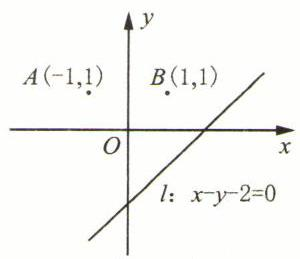
\includegraphics[width=0.2\textwidth]{bodyxb/src/bo_d20cdrf7aajc73bfmvhg_41_1168_438_300_259_0.jpg}
\end{center}


(第 93 题)

$\because \;\Delta  = {3}^{2} - 4 \times  4 =  - 7 < 0,\;\therefore \;{PA}$ 与 ${PB}$ 不垂直,当 $t - 2 \leq  1$ 即 $t \leq  3$ 时, $\angle {APB}$ 是 ${PB}$ 到 ${PA}$ 的角,

$\therefore \tan \angle {APB} = \dfrac{{k}_{PA} - {k}_{PB}}{1 + {k}_{PA} \cdot  {k}_{PB}} = \dfrac{3 - t}{{t}^{2} - {3t} + 4}$ . 当 $t > 3$ 时, $\angle {APB}$ 是 ${PA}$ 到 ${PB}$ 的角,

$\therefore \tan \angle {APB} = \dfrac{{k}_{PB} - {k}_{PA}}{1 + {k}_{PA} \cdot  {k}_{PB}} = \dfrac{t - 3}{{t}^{2} - {3t} + 4}$ . 当 $t =  - 1$ 时, $P\left( {-1, - 3}\right) ,{PA} \bot  x$ 轴,其倾斜角为 ${90}^{ \circ  }$ ,而 ${k}_{PB} = \dfrac{1 + 3}{1 + 1} = 2$ ,其倾斜角为 $\arctan 2,\tan \angle {APB} = \tan \left( {\dfrac{\pi }{2} - \arctan 2}\right)  = \tan \left( {\arctan \dfrac{1}{2}}\right)  = \dfrac{1}{2} =$  $\dfrac{3 - \left( {-1}\right) }{{\left( -1\right) }^{2} - 3\left( {-1}\right)  + 4}$ . 当 $t = 1$ 时, $P\left( {1, - 1}\right) ,{PB} \bot  x$ 轴,其倾斜角为 ${90}^{ \circ  },{k}_{PA} = \dfrac{1 + 1}{-1 - 1} =  - 1$ ,其倾斜角为 $\arctan \left( {-1}\right)  + \pi$  $= \dfrac{3}{4}\pi ,\tan \angle {APB} = \tan \left( {\dfrac{3}{4}\pi  - \dfrac{\pi }{2}}\right)  = \tan \dfrac{1}{4}\pi  = 1.\;\therefore \;\tan \angle {APB} = \dfrac{\left| t - 3\right| }{{t}^{2} - {3t} + 4}\left( {t \in  \mathbf{R}}\right)$ . 令 ${t}^{\prime } = t - 3 \in  \mathbf{R}$

此时 $\tan \angle {APB} = \dfrac{\left| {t}^{\prime }\right| }{{t}^{\prime 2} + 3{t}^{\prime } + 4} = \left\{  \begin{array}{l} \dfrac{1}{{t}^{\prime } + \dfrac{4}{{t}^{\prime }} + 3} \leq  \dfrac{1}{2\sqrt{{t}^{\prime } \cdot  \dfrac{4}{{t}^{\prime }}} + 3} = \dfrac{1}{7},{t}^{\prime } > 0, \\  \dfrac{1}{-{t}^{\prime } + \left( {-\dfrac{4}{{t}^{\prime }}}\right)  - 3} \leq  \dfrac{1}{2\sqrt{\left( {-{t}^{\prime }}\right)  \cdot  \left( {-\dfrac{4}{{t}^{\prime }}}\right) } - 3} = 1,{t}^{\prime } < 0. \end{array}\right.$

$\angle {APB} \in  \lbrack 0,\pi ),\therefore \angle {APB}$ 最大为 $\operatorname{arctanl} = \dfrac{\pi }{4}$ . 此时 $- {t}^{\prime } =  - \dfrac{4}{{t}^{\prime }}$ ,且 ${t}^{\prime } < 0,\therefore {t}^{\prime } =  - 2,\therefore t = 1$ ,

$\therefore P\left( {1, - 1}\right)$ .

综上,当 $P$ 取(1, - 1)时, $\angle {APB}$ 取最大值 $\dfrac{\pi }{4}$ .

注: 如果用余弦定理写出 $\cos \angle {APB}$ 的值,尽管不用单独讨论 $t =  \pm  1$ 时的情况,但求 $\cos \angle {APB}$ 的值域远不如求 $\tan \angle {APB}$ 的值域方便.

94. 集合 $A$ 表示的是直线 ${l}_{1}$ 且不经过点(2,3),其中 ${l}_{1} : \left( {a + 1}\right) x - y + \left( {1 - {2a}}\right)  = 0,\left( {x,y}\right)  \neq  \left( {2,3}\right)$ . 对于集合 $B$ ,当 $\left\{  \begin{array}{l} {a}^{2} - 1 = 0, \\  a - 1 = 0, \end{array}\right.$ 即 $a = 1$ 时, $B = \varnothing$ ,此时 $A \cap  B = \varnothing$ . 当 $a \neq  1$ 时, $B$ 表示一条直线 ${l}_{2} : \left( {{a}^{2} - 1}\right) x + \left( {a - 1}\right) y - {15} = 0$ .

此时 ${l}_{1} : y = \left( {a + 1}\right) x + \left( {1 - {2a}}\right) ,{l}_{2} : y =  - \left( {a + 1}\right) x + \dfrac{15}{a - 1}.{l}_{1}$ 与 ${l}_{2}$ 的位置关系必居以下两者之一:

① ${l}_{1}//{l}_{2}$ ,此时 $\left\{  \begin{array}{l} a + 1 =  - \left( {a + 1}\right) , \\  1 - {2a} \neq  \dfrac{15}{a - 1}, \end{array}\right.$ 解得 $a =  - 1$ .

② ${l}_{1}$ 与 ${l}_{2}$ 相交,此时 $a + 1 \neq   - \left( {a + 1}\right)$ ,即 $a \neq   - 1$ . 为使 $A \cap  B \neq  \varnothing$ ,则 ${l}_{2}$ 应过点(2,3),将(2,3)代入 ${l}_{2}$ ,有 $2\left( {{a}^{2} - 1}\right)  +$  $3\left( {a - 1}\right)  = {15}$ ,解得 ${a}_{1} =  - 4,{a}_{2} = \dfrac{5}{2}$ (均满足 $a \neq   \pm  1$ ). 综上,当 $a = 1$ 或 $a =  - 1$ 或 $a =  - 4$ 或 $a = \dfrac{5}{2}$ 时,有 $A \cap  B = \varnothing$ .

95. 点 $A$ 关于 $\angle {ABC},\angle {ACB}$ 的平分线所在直线的对称的点一定在直线 ${BC}$ 上.

记 ${l}_{1} : x - {2y} = 0,{l}_{2} : x + y - 1 = 0$ ,斜率分别为 ${k}_{1} = \dfrac{1}{2},{k}_{2} =  - 1$ . 记点 $A$ 关于 ${l}_{1},{l}_{2}$ 对称的点分别为 ${A}^{\prime }$ 和 ${A}^{\prime \prime }.A{A}^{\prime }\bot {l}_{1}$ , $A{A}^{\prime \prime } \bot  {l}_{2},\;\therefore \;{k}_{A{A}^{\prime }} =  - \dfrac{1}{{k}_{1}} =  - 2,{k}_{A{A}^{\prime }} =  - \dfrac{1}{{k}_{2}} = 1,\;\therefore \;{l}_{A{A}^{\prime }} : y - 4 =  - 2\left( {x - 1}\right)$ ,即 ${2x} + y - 6 = 0,{l}_{A{A}^{\prime \prime }} : y - 4 = 1 \cdot  (x$  $- 1)$ ,即 $x - y + 3 = 0.A{A}^{\prime }$ 与 ${l}_{1}$ 的交点满足 $\left\{  \begin{array}{l} {2x} + y - 6 = 0, \\  x - {2y} = 0. \end{array}\right.$ 即点 $\left( {\dfrac{12}{5},\dfrac{6}{5}}\right)$ . 这是线段 $A{A}^{\prime }$ 的中点,故 ${A}^{\prime }$

$\left( {\dfrac{12}{5} \times  2 - 1,\dfrac{6}{5} \times  2 - 4}\right)$ ,即 ${A}^{\prime }\left( {\dfrac{19}{5}, - \dfrac{8}{5}}\right)$ . 同样地, $A{A}^{\prime \prime }$ 与 ${l}_{2}$ 的交点满足 $\left\{  \begin{array}{l} x - y + 3 = 0, \\  x + y - 1 = 0, \end{array}\right.$ 即点(-1,2),故 ${A}^{\prime \prime }( - 1 \times  2 -$  $1,2 \times  2 - 4)$ ,即 ${A}^{\prime \prime }\left( {-3,0}\right)$ ,过点 ${A}^{\prime }{A}^{\prime \prime }$ 的直线即为过点 $B,C$ 的直线, $\therefore {l}_{BC} : \dfrac{y - 0}{-\dfrac{8}{5} - 0} = \dfrac{x + 3}{\dfrac{19}{5} + 3}$ ,即 ${l}_{BC} : {4x} + {17y} + {12}$  $= 0$ .

96. 第一步:先弄清 ${l}_{1},{l}_{2}$ 及 $A,B$ 相互间的位置关系:

\begin{center}
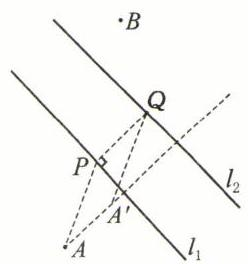
\includegraphics[width=0.2\textwidth]{bodyxb/src/bo_d20cdrf7aajc73bfmvhg_42_1291_348_248_264_0.jpg}
\end{center}


(第 96 题)

如图 ${l}_{1}$ 在 ${l}_{2}$ 下方,点 $A$ 在 ${l}_{1}$ 下方,点 $B$ 在 ${l}_{2}$ 上方.

第二步:下面从几何角度讨论. ‘ 两平行直线间的距离 $\therefore \left| {AP}\right|  + \left| {PQ}\right|  + \left| {QB}\right|$ 最小 $\Leftrightarrow$  $\left| {AP}\right|  + \left| {QB}\right|$ 最小. 在 ${l}_{2}$ 上任意取一点 $Q$ ,对应得到 $Q$ 在 ${l}_{1}$ 上的射影 $P$ ,考虑将 $\vv{PA}$ 的起点移到点 $Q$ . 为此,过点 $A$ 向 ${l}_{1}$ 引垂线,并取点 ${A}^{\prime }$ ,使 $\vv{A{A}^{\prime }} = \vv{PQ}$ ,易知 $A{A}^{\prime } ⫫ {PQ}$ ,故四边形 $A{A}^{\prime }{QP}$ 是平行四边形, $\therefore {PA} ⫫ Q{A}^{\prime }$ (即 $\vv{PA} = \vv{Q{A}^{\prime }}$ ). 注意到,由于点 $A$ 到 ${l}_{2}$ 的距离大于 $\left| {PQ}\right|$ ,故 ${A}^{\prime }$ 与 $B$ 一定在 ${l}_{2}$ 的两侧 (当然 ${A}^{\prime }$ 可能会在 ${l}_{1}$ 上或 ${l}_{1}$ 与 ${l}_{2}$ 之间). 这样, $\left| {AP}\right|  + \left| {QB}\right|  = \left| {{A}^{\prime }Q}\right|  +$  $\left| {QB}\right|  \geq  \left| {{A}^{\prime }B}\right|$ . 当且仅当点 $Q$ 为 ${A}^{\prime }B$ 与 ${l}_{2}$ 交点时等号成立.

第三步: ${l}_{1}$ 与 ${l}_{2}$ 的距离 $\left| {PQ}\right|  = \dfrac{\left| {10} + {15}\right| }{\sqrt{{3}^{2} + {4}^{2}}} = 5,\because {l}_{1},{l}_{2}$ 斜率为 ${k}_{1} = {k}_{2} =  - \dfrac{3}{4}$ ,而 $A{A}^{\prime }\bot {l}_{1},\therefore {k}_{A{A}^{\prime }} =  - \dfrac{1}{{k}_{1}} = \dfrac{4}{3}$ ,

$\therefore {l}_{A{A}^{\prime }} : y + 8 = \dfrac{4}{3}\left( {x + 3}\right)$ 即 ${4x} - {3y} - {12} = 0$ . 设 ${A}^{\prime }$ 的坐标为 $\left( {m,n}\right) .\;\because$ 点 $A$ 到 ${l}_{1}$ 的距离为 $\dfrac{\left| -9 - {32} + {10}\right| }{\sqrt{{3}^{2} + {4}^{2}}} = \dfrac{31}{5}$ ,

$\therefore$ 点 ${A}^{\prime }$ 到 ${l}_{1}$ 的距离为 $\dfrac{\left| 3m + 4n + {10}\right| }{\sqrt{{3}^{2} + {4}^{2}}} = \left| {\dfrac{31}{5} - 5}\right|  = \dfrac{6}{5}$ ,联立 $\left\{  \begin{array}{l} \dfrac{\left| 3m + 4n + {10}\right| }{5} = \dfrac{6}{5}, \\  {l}_{A{A}^{\prime }} : {4m} - {3n} - {12} = 0, \end{array}\right.$ 解得 $\left\{  \begin{array}{l} m = \dfrac{36}{25}, \\  n =  - \dfrac{52}{25}, \end{array}\right.$ 或 $\left\{  \begin{array}{l} m = 0, \\  n =  - 4. \end{array}\right.$ 另一方面, $\because \left| {A{A}^{\prime }}\right|  = 5,\therefore \left\{  \begin{array}{l} m = \dfrac{36}{25}, \\  n =  - \dfrac{52}{25}. \end{array}\right.$ 不合题意, $\therefore {A}^{\prime }\left( {0, - 4}\right) ,\therefore {l}_{{A}^{\prime }B} : \dfrac{y + 4}{4 + 4} = \dfrac{x - 0}{{10} - 0}$ ,即 ${4x} - {5y} - {20} = 0$ , 联立 $\left\{  \begin{array}{l} {4x} - {5y} - {20} = 0, \\  {3x} + {4y} - {15} = 0, \end{array}\right.$ 解得 $\left\{  {\begin{array}{l} x = 5, \\  y = 0. \end{array}\;\therefore \;Q\left( {5,0}\right) .\;\therefore \;\vv{{A}^{\prime }Q} = \left( {5,0}\right)  - \left( {0, - 4}\right)  = \left( {5,4}\right) }\right.$ ,由 $\vv{AP} = \vv{{A}^{\prime }Q}$ 及 $A\left( {-3, - 8}\right)$ , $\therefore P\left( {-3 + 5, - 8 + 4}\right)$ ,即 $P\left( {2, - 4}\right)$ . 由 $A\left( {-3, - 8}\right) ,P\left( {2, - 4}\right) ,Q\left( {5,0}\right) ,B\left( {{10},4}\right)$ ,写出 ${l}_{AP} : \dfrac{y + 4}{-8 + 4} = \dfrac{x - 2}{-3 - 2}$ ,即 ${4x} - {5y} - {28} = 0,{l}_{PQ} : \dfrac{y - 0}{-4 - 0} = \dfrac{x - 5}{2 - 5}$ ,即 ${4x} - {3y} - {20} = 0,{l}_{QB} : \dfrac{y - 0}{4 - 0} = \dfrac{x - 5}{{10} - 5}$ ,即 ${4x} - {5y} - {20} = 0$ . 此时有 $\left| {AP}\right|  + \left| {PQ}\right|  +$  $\left| {QB}\right|$ 的最小值为 $\sqrt{{5}^{2} + {4}^{2}} + 5 + \sqrt{{5}^{2} + {4}^{2}}$ ,即 ${\left( \left| AP\right|  + \left| PQ\right|  + \left| QB\right| \right) }_{\min } = 5 + 2\sqrt{41}$ .

97. (1) ${l}_{1}$ 过 (且仅过) 定点 $A\left( {0,1}\right) .{l}_{2}$ 过 (且仅过) 定点 $B\left( {1,0}\right)$ .

(2)联立 $\left\{  \begin{array}{l} y = {mx} + 1, \\  x =  - {my} + 1, \end{array}\right.$ 解得 $\left\{  \begin{array}{l} x = \dfrac{1 - m}{{m}^{2} + 1}, \\  y = \dfrac{m + 1}{{m}^{2} + 1}. \end{array}\right.$ , $\therefore$ 点 $P$ 的坐标为 $\left( {\dfrac{1 - m}{{m}^{2} + 1},\dfrac{m + 1}{{m}^{2} + 1}}\right)$ .

(3) 由 $A\left( {0,1}\right) ,B\left( {1,0}\right)$ 知 $\left| {AB}\right|  = \sqrt{{1}^{2} + {1}^{2}} = \sqrt{2},{l}_{AB} : \dfrac{y - 0}{1 - 0} = \dfrac{x - 1}{0 - 1}$ ,即 $x + y - 1 = 0$ . 点 $P$ 到 ${l}_{AB}$ 的距离为 $h =$  $\dfrac{\left| \dfrac{1 - m}{{m}^{2} + 1} + \dfrac{m + 1}{{m}^{2} + 1} - 1\right| }{\sqrt{{1}^{2} + {1}^{2}}} = \dfrac{1}{\sqrt{2}} \cdot  \dfrac{\left| 1 - {m}^{2}\right| }{{m}^{2} + 1}.\;\because \;\left| m\right|  < 1,\;\therefore \;h = \dfrac{1}{\sqrt{2}} \cdot  \dfrac{1 - {m}^{2}}{{m}^{2} + 1},$

$\therefore S = \dfrac{1}{2} \cdot  \left| {AB}\right|  \cdot  h = \dfrac{1}{2} \cdot  \dfrac{1 - {m}^{2}}{{m}^{2} + 1}\left( {\left| m\right|  < 1}\right)$ .

(4) $\left| m\right|  < 1$ 时,记 $t = {m}^{2} \in  \lbrack 0,1).\;\therefore \;S = \dfrac{1}{2} \cdot  \dfrac{1 - {m}^{2}}{{m}^{2} + 1} = \dfrac{1}{2} \cdot  \dfrac{-t + 1}{t + 1} = \dfrac{1}{2}\left( {-1 + \dfrac{2}{t + 1}}\right)$ . 易见 $S \in  \left( {0,\dfrac{1}{2}}\right\rbrack  ,{S}_{\max } = \dfrac{1}{2}$ . 相应地, $m = 0$ .

98. (约定系数法). 原方程为二次式,而直线方程为一次式,故原方程可写为 $\left( {{A}_{1}x + {B}_{1}y + {C}_{1}}\right) \left( {{A}_{2}x + {B}_{2}y + {C}_{2}}\right)  = 0$ . 对比系

数,有 $\left\{  \begin{array}{ll} {A}_{1}{C}_{2} = a, & \text{ ① } \\  {A}_{1}{B}_{2} + {A}_{2}{B}_{1} =  - 4, & \text{ ② } \\  {B}_{1}{C}_{2} + {A}_{2}{C}_{1} = 3\sqrt{3}, & \text{ ③ } \\  {A}_{1}{C}_{2} + {A}_{2}{C}_{1} = 3\sqrt{3}, & \text{ ④ } \\  {B}_{1}{C}_{2} + {B}_{2}{C}_{1} =  - 3, & \text{ ⑤ } \\  {C}_{1}{C}_{2} = 0, & \text{ ⑥ } \end{array}\right.$ 首先由⑥知 ${C}_{1} = 0$ . 此时④⑤即为④, ${A}_{2}{C}_{1} = 3$ . 此时④⑤即为④, ${A}_{2}{C}_{1} = 3\sqrt{3},$ ⑤

${B}_{2}{C}_{1} =  - 3$ ,消去 ${C}_{1}$ 得 ${A}_{2} =  - \sqrt{3}{B}_{2}$ . 代入 ②,结合③ 有 ${A}_{1}{B}_{2} - \sqrt{3}{B}_{1}{B}_{2} = {A}_{1}{B}_{2} - \sqrt{3} \cdot  \sqrt{3} =  - 4,\therefore {A}_{1}{B}_{2} =  - 1$ . 代入②,相应地 ${A}_{2}{B}_{1} =  - 3,\therefore \left( {{A}_{1}{B}_{2}}\right)  \cdot  \left( {{A}_{2}{B}_{1}}\right)  = \left( {{A}_{1}{A}_{2}}\right)  \cdot  \left( {{B}_{1}{B}_{2}}\right)  = 3$ ,再代入①③,有 $a \cdot  \sqrt{3} = 3,\therefore a = \sqrt{3}$ . 进一步令 ${C}_{1} = k\left( {k \neq  0,k\text{ 为常数 }}\right)$ ,有 $\left\{  \begin{array}{l} {A}_{1} = \dfrac{k}{3}, \\  {A}_{2} = \dfrac{k}{3}, \\  {B}_{1} =  - \dfrac{k}{\sqrt{3}}, \\  {B}_{2} =  - \dfrac{3}{4}, \\  {C}_{1} = k, \\  {C}_{2} = 0, \\  {C}_{3} = 0. \end{array}\right. \therefore$ 原方程可写 $\left( {\dfrac{k}{3}x - \dfrac{k}{\sqrt{3}}y + k}\right) \left( {\dfrac{3\sqrt{3}}{k}x - \dfrac{k}{k}y + k}\right) \left( {\dfrac{3\sqrt{3}}{k}x - \dfrac{3}{k}y}\right)  = 0$ ,即 $(x - \sqrt{3}y +$

3) $\left( {\sqrt{3}x - y}\right)  = 0,\;\therefore \;a = \sqrt{3}$ 时,原方程表示两条直线.

99. 函数 ${y}_{2} = \dfrac{\left| x\right|  - 1}{\left| x - 1\right| }$ 的定义域为 $\left( {-\infty ,1}\right)  \cup  \left( {1, + \infty }\right) ,{y}_{2} = \left\{  \begin{array}{l} 1,x > 1, \\   - 1,0 < x < 1, \\  \dfrac{-x - 1}{1 - x},x \leq  0. \end{array}\right.$

①当 $x > 1$ 时,将 ${y}_{2} = 1$ 代入 ${y}_{1} = {mx}$ . 当 $m \neq  0$ 时, $x = \dfrac{1}{m},{y}_{1}$ 与 ${y}_{2}$ 没有公共点,则 $\left\{  \begin{array}{l} \dfrac{1}{m} \leq  1, \\  m \neq  0. \end{array}\right.$ 得 $m \in  \left( {-\infty ,0}\right)  \cup  \lbrack 1, + \infty )$ . 另外, $m = 0$ 时, ${y}_{1} = 0$ 和 ${y}_{2} = 1$ 在 $x > 1$ 时无公共点. 因此, $m \in  \left( {-\infty ,0}\right\rbrack   \cup  \lbrack 1, + \infty )$ .

②当 $0 < x < 1$ 时,将 ${y}_{2} =  - 1$ 代入 ${y}_{1} = {mx}$ . 当 $m \neq  0$ 时, $x =  - \dfrac{1}{m}$ . ${y}_{1}$ 与 ${y}_{2}$ 没有公共点,则 $\left\{  \begin{array}{l}  - \dfrac{1}{m} \leq  0\text{ 或 } - \dfrac{1}{m} \geq  1, \\  m \neq  0. \end{array}\right.$ 得 $m \in$  $\lbrack  - 1,0) \cup  \left( {0, + \infty }\right)$ . 同样,当 $m = 0$ 时, ${y}_{1} = 0$ 和 ${y}_{2} = 1$ 在 $0 < x < 1$ 时无公共点, $\;\therefore \;$ 因此, $m \in  \lbrack  - 1, + \infty )$ . ③当 $x \leq  0$ 时, $\left\{  \begin{array}{l} {y}_{1} = {mx}, \\  {y}_{2} = \dfrac{-x - 1}{1 - x}. \end{array}\right.$ 整理得 $m{x}^{2} - \left( {m + 1}\right) x - 1 = 0$ . 当 $m = 0$ 时,方程为一次方程,有公共点(-1,0)符合 $x \leq  0$ , $m \neq  0$ 时,方程为二次方程. 如果方程有实根 $\left( {\Delta  \geq  0}\right)$ ,则 $\left\{  \begin{array}{l} {x}_{1} + {x}_{2} = \dfrac{m + 1}{2m}, \\  {x}_{1}{x}_{2} =  - \dfrac{1}{m}. \end{array}\right.$ 由①②,得 $m \in  \left\lbrack  {-1,0}\right\rbrack   \cup  \lbrack 1, + \infty )$ . 当 $m \in  \lbrack 1$ , $+ \infty )$ 时, ${x}_{1}{x}_{2} =  - \dfrac{1}{m} < 0$ ,故在 $x \leq  0$ 上必有解. 当 $m \in  \left\lbrack  {-1,0}\right\rbrack$ 时, ${x}_{1} + {x}_{2} = \dfrac{m + 1}{2m} \leq  0$ ,故至少有一个实根小于等于 0 . 在 $x \leq  0$ 时必有解, $\therefore m \neq  0$ 时, $\Delta  = {\left( m + 1\right) }^{2} + {4m} < 0$ ,方程没有实根, $m \in  \left( {-3 - 2\sqrt{2}, - 3 + 2\sqrt{2}}\right)$ .

综合①②③, $m \in  \lbrack  - 1, - 3 + 2\sqrt{2})$ .

100. 记 ${\log }_{3}a = u$ ,则函数可表示为 $y = \left( {x - 1}\right)  \cdot  {t}^{2} - {6t} \cdot  x + x + 1$ ,即 $y = \left( {{t}^{2} - {6t} + 1}\right) x + \left( {1 - {t}^{2}}\right)$ 是一条直线方程,记为直线 $l : y = f\left( x\right)$ ,不难得出 $l$ 在 $x \in  \left\lbrack  {0,1}\right\rbrack$ 内恒正 $\Leftrightarrow  \left\{  \begin{array}{l} f\left( 0\right)  > 0, \\  f\left( 1\right)  > 0. \end{array}\right.$ (充分性由题意知,必要性由图形及几何易得) $\left\{  {\begin{array}{l} f\left( 0\right)  = 1 - {t}^{2} > 0, \\  f\left( 1\right)  =  - {6t} + 2 > 0. \end{array}\;\therefore \; - 1 < t < \dfrac{1}{3},\;\therefore \; - 1 < {\log }_{3}a < \dfrac{1}{3},\;\therefore \;\dfrac{1}{3} < a < \sqrt[3]{3}.}\right.$

101. (1) 如图,不妨设 $\bigtriangleup {AOB}$ 的顶点 $O$ 为原点. 记 $A,B$ 两点的坐标分别为 $A\left( {{x}_{1},{y}_{1}}\right) ,B\left( {{x}_{2},{y}_{2}}\right)$ ,易知 $M\left( {\dfrac{{x}_{2}}{2},\dfrac{{y}_{2}}{2}}\right)$ ,

$N\left( {\dfrac{{x}_{1}}{2},\dfrac{{y}_{1}}{2}}\right) ,\left| {AM}\right|  = \left| {BN}\right|  \Leftrightarrow  {\left( {x}_{1} - \dfrac{{x}_{2}}{2}\right) }^{2} + {\left( {y}_{1} - \dfrac{{y}_{2}}{2}\right) }^{2} = {\left( {x}_{2} - \dfrac{{x}_{1}}{2}\right) }^{2} + {\left( {y}_{2} - \dfrac{{y}_{1}}{2}\right) }^{2} \Leftrightarrow  {x}_{1}^{2} + {y}_{1}^{2} = {x}_{2}^{2} + {y}_{2}^{2} \Leftrightarrow  {\left| OA\right| }^{2} =$  ${\left| OB\right| }^{2} \Leftrightarrow  \left| {OA}\right|  = \left| {OB}\right| ,\therefore \bigtriangleup {OAB}$ 是等腰三角形, $\therefore$ 两条中线相等的三角形是等腰三角形, 证毕.

\begin{center}
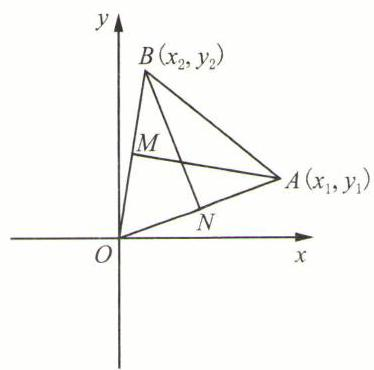
\includegraphics[width=0.3\textwidth]{bodyxb/src/bo_d20cdrf7aajc73bfmvhg_44_1158_126_374_370_0.jpg}
\end{center}


[第 101(1)题]

(2)由题意,设正方形 ${ABCD}$ 的边长为 $a$ ,则 $A\left( {0,a}\right)$ , $B\left( {a,a}\right)$ , $C\left( {a,0}\right)$ , $D\left( {0,0}\right)$ .

$\because {AC}//{DE}$ ,且 $\angle {ACD} = {45}^{ \circ  },\;\therefore \;$ 设点 $E$ 的坐标为 $E\left( {-x,x}\right) ,\left| {CE}\right|  =$  $\left| {AC}\right|  \Leftrightarrow  {\left( -x - a\right) }^{2} + {x}^{2} = 2{a}^{2},\;\therefore 2{x}^{2} + {2ax} - {a}^{2} = 0$ ,结合 $x > 0$ 得 $x =$  $\dfrac{\sqrt{3} - 1}{2}a$

设点 $F$ 的坐标为 $F\left( {0,y}\right)$ ,及 $\vv{EF} = \lambda \vv{FC}$ . 根据定比分点公式,

$F\left( {\dfrac{-x + {\lambda a}}{1 + \lambda },\dfrac{x}{1 + \lambda }}\right) ,\;\therefore \;\left\{  {\begin{array}{l} 0 = \dfrac{-x + {\lambda a}}{1 + \lambda }, \\  y = \dfrac{x}{1 + \lambda }, \end{array}\text{ 解得 }\left\{  \begin{array}{l} \lambda  = \dfrac{x}{a}, \\  y = \dfrac{ax}{a + x}. \end{array}\right. }\right.$

$\therefore F\left( {0,\dfrac{ax}{a + x}}\right)$ .

${\left| AF\right| }^{2} = {\left( \dfrac{ax}{a + x} - a\right) }^{2} = {\left( \dfrac{{a}^{2}}{a + x}\right) }^{2},{\left| AE\right| }^{2} = {\left( -x\right) }^{2} + {\left( x - a\right) }^{2} = 2{x}^{2} - {2ax} + {a}^{2}$ . 将 ${a}^{2} = 2{x}^{2} + {2ax}$ 和 $- {2ax} + {a}^{2} =$  $2{x}^{2}$ 分别代入 ${\left| AF\right| }^{2}$ 和 ${\left| AE\right| }^{2}$ ,有 ${\left| AF\right| }^{2} = {\left( \dfrac{{2x}\left( {a + x}\right) }{a + x}\right) }^{2} = 4{x}^{2},{\left| AE\right| }^{2} = 2{x}^{2} + 2{x}^{2} = 4{x}^{2}$ ,

$\therefore {\left| AF\right| }^{2} = {\left| AE\right| }^{2}$ ,即 $\left| {AF}\right|  = \left| {AE}\right|$ ,证毕.

102. (1) 方法一: 原直线方程整理得 $l : \left( {\lambda  + 2}\right) x - \left( {\lambda  + 1}\right) y - \left( {{4\lambda } + 6}\right)  = 0$ . 点 $P\left( {3, - 1}\right)$ 与直线 $l$ 的距离 $d =$  $\dfrac{\left| 3\left( \lambda  + 2\right)  + \left( \lambda  + 1\right)  - \left( 4\lambda  + 6\right) \right| }{\sqrt{{\left( \lambda  + 2\right) }^{2} + {\left( \lambda  + 1\right) }^{2}}} = \dfrac{1}{\sqrt{2{\lambda }^{2} + {6\lambda } + 5}}$ . 若 $d = 3$ ,则 $\dfrac{1}{\sqrt{2{\lambda }^{2} + {6\lambda } + 5}} = 3 \Leftrightarrow  1 = 9\left( {2{\lambda }^{2} + {6\lambda } + 5}\right)  \Rightarrow  {18}{\lambda }^{2} + {54\lambda } +$  ${44} = 0$ . 其 $\Delta  = {54}^{2} - 4 \times  {18} \times  {44} =  - {252} < 0,\;\therefore \;d \neq  3$ ,证毕.

方法二: 由方法一,我们进一步分析 $d,d = \dfrac{1}{\sqrt{2{\lambda }^{2} + {6\lambda } + 5}} = \dfrac{1}{\sqrt{2{\left( \lambda  + \dfrac{3}{2}\right) }^{2} + \dfrac{1}{2}}}$ ,对 $\forall \lambda  \in  \mathbf{R},2{\left( \lambda  + \dfrac{3}{2}\right) }^{2} + \dfrac{1}{2} \geq  \dfrac{1}{2}$ , $\therefore d \leq  \dfrac{1}{\sqrt{\dfrac{1}{2}}}$ ,即 $d \leq  \sqrt{2},\therefore d$ 恒不等于 3,证毕. 方法三:记 ${l}_{1} : {2x} - y - 6 = 0,{l}_{2} : x - y - 4 = 0$ ,故 $l : {2x} - y - 6 + \lambda \left( {x - y - 4}\right)  = 0$ 是过 ${l}_{1},{l}_{2}$ 的交点的直线系(不含 $\left. {l}_{2}\right)$ . 联立 $\left\{  \begin{array}{l} {2x} - y - 6 = 0, \\  x - y - 4 = 0, \end{array}\right.$ 解得 $\left\{  {\begin{array}{l} x = 2, \\  y =  - 2. \end{array}\therefore }\right. \;{l}_{1},{l}_{2}$ 的交点为 $Q\left( {2, - 2}\right)$ . 即使包含 ${l}_{2}$ ,过交点 $Q$ 的直线系与点 $P$ (3, - 1)的最大距离为 $\left| {PQ}\right|  = \sqrt{{\left( 2 - 3\right) }^{2} + {\left( -2 - \left( -1\right) \right) }^{2}} = \sqrt{2} < 3$ .

$\therefore$ 直线 $l$ 与点 $P$ 的距离恒不等于 3 .

(2) 由题意, $d = \dfrac{\left| -2\left( 2 + k\right)  - 2\left( 1 + k\right)  - 2\left( 3 + 2k\right) \right| }{\sqrt{{\left( 2 + k\right) }^{2} + {\left( 1 + k\right) }^{2}}} = \dfrac{8\left| {k + \dfrac{3}{2}}\right| }{\sqrt{2{k}^{2} + {6k} + 5}} = \dfrac{8\left| {k + \dfrac{3}{2}}\right| }{\sqrt{2{\left( k + \dfrac{3}{2}\right) }^{2} + \dfrac{1}{2}}}$ . 令 $t = k + \dfrac{3}{2}$ .

$\because k \in  \mathbf{R},\;\therefore t \in  \mathbf{R},\;\therefore d = \dfrac{8\left| t\right| }{\sqrt{2{t}^{2} + \dfrac{1}{2}}},t = 0$ 时, $d = 0;t \neq  0$ 时, $d = \dfrac{8}{\sqrt{2 + \dfrac{1}{2{t}^{2}}}}$ . 此时 ${t}^{2} \in  \left( {0, + \infty }\right)$ ,

$\therefore d \in  \left( {0,\dfrac{8}{\sqrt{2}}}\right)$ ,即 $d \in  \left( {0,4\sqrt{2}}\right) .\;\therefore$ 当 $k \in  \mathbf{R}$ 时, $d \in  \left\lbrack  {0,4\sqrt{2}}\right) \;\therefore d$ 不能大于或等于 $4\sqrt{2}$ ,证毕.

103. (1) 方法一:将原直线整理为 $l : m\left( {x + {2y} - 1}\right)  - \left( {x + y - 5}\right)  = 0$ ,是过 ${l}_{1} : x + {2y} - 1 = 0$ 和 ${l}_{2} : x + y - 5 = 0$ 交点 $M$ 的直线系 (不含 ${l}_{1}$ ). 由 $\left\{  \begin{array}{l} x + {2y} - 1 = 0, \\  x + y - 5 = 0, \end{array}\right.$ 解得 $\left\{  {\begin{array}{l} x = 9, \\  y =  - 4. \end{array}\;\therefore }\right.$ 直线 $l$ 恒过定点(9, - 4),证毕.

方法二: 令 $m = 1$ ,有直线 $y =  - 4$ ,令 $m = \dfrac{1}{2}$ ,有直线 $x = 9$ . 这两条直线交于点(9, - 4). 将(9, - 4)代入原直线,左边 $= \left( {m - 1}\right)  \cdot  9 - 4 \cdot  \left( {{2m} - 1}\right)  = m - 5$ ,右边 $= m - 5$ . 左边恒等于右边,故原直线恒过定点(9, - 4),证毕.

(2)将 $p + {2q} - 1 = 0$ 即 $p = 1 - {2q}$ 代入原直线方程,得 $\left( {1 - {2q}}\right) x + {3y} + q = 0$ . 令 $q = \dfrac{1}{2}$ ,则有直线 $y =  - \dfrac{1}{6}$ ,令 $q = 0$ ,则有直线 $x + {3y} = 0$ . 由 $\left\{  \begin{array}{l} y =  - \dfrac{1}{6}, \\  x + {3y} = 0, \end{array}\right.$ 解得 $\left\{  \begin{array}{l} x = \dfrac{1}{2}, \\  y =  - \dfrac{1}{6}. \end{array}\right.$ 即点 $\left( {\dfrac{1}{2}, - \dfrac{1}{6}}\right)$ ,将点 $\left( {\dfrac{1}{2}, - \dfrac{1}{6}}\right)$ 代入 ${px} + {3y} + q$ ,有 $\dfrac{1}{2}p - \dfrac{1}{2}$

$+ q = \dfrac{1}{2}\left( {p + {2q} - 1}\right)  = 0.\;\therefore$ 直线 ${px} + {3y} + q = 0$ 恒过定点 $\left( {\dfrac{1}{2}, - \dfrac{1}{6}}\right)$ ,证毕.

(3)将原直线整理为 $m\left( {{2x} + {3y} - {18}}\right)  + n\left( {x - {2y} + 5}\right)  = 0.\because m,n$ 不同时为 0, $\therefore$ 令 $m = 0$ 时,有直线 $x - {2y} +$  $5 = 0$ ,令 $n = 0$ 时,有直线 ${2x} + {3y} - {18} = 0$ . 由 $\left\{  \begin{array}{l} x - {2y} + 5 = 0, \\  {2x} + {3y} - {18} = 0, \end{array}\right.$ 解得 $\left\{  \begin{array}{l} x = 3, \\  y = 4. \end{array}\right.$

将 $M\left( {3,4}\right)$ 代入 $\left( {{2m} + n}\right) x + \left( {{3m} - {2n}}\right) y - {18m} + {5n} = {6m} + {3n} + {12m} - {8n} - {18m} + {5n} = 0,\therefore$ 原直线恒过定点 (3,4),证毕.

